
\documentclass{article}
\usepackage[utf8]{inputenc}
\usepackage{mathtools}
\usepackage{amssymb}
\usepackage{amsmath}
\usepackage{listings}
\usepackage{braket}
\usepackage[toc,page]{appendix}

%%%THEOREM (ETC) ENVIRONMENTS
\newtheorem{definition}{Definition}
\newtheorem{claim}{Claim}
\newtheorem{conjecture}{Conjecture}
\newtheorem{corollary}{Corollary}
\newtheorem{example}{Example}
\newtheorem{problem}{Problem}
\newtheorem{idea}{Idea} 

\usepackage{proof}
\newtheorem{theorem}{Theorem}

\newtheorem{lemma}[theorem]{Lemma}
\newtheorem{proposition}[theorem]{Proposition}

\newenvironment{proof}[1][Proof]{\begin{trivlist}
\item[\hskip \labelsep {\bfseries #1}]}{\begin{flushright}$\blacksquare$\end{flushright} \end{trivlist}}
\newenvironment{remark}[1][Remark]{\begin{trivlist}
\item[\hskip \labelsep {\bfseries #1}]}{\end{trivlist}}

\newcommand{\cat}{\mathcal{C}}
\newcommand{\Tau}{\mathrm{T}}
\newcommand{\ham}{\mathcal{H}}
\title{Hopf Algebras in Quantum Computation}
\author{Giovanni de Felice}
\date{April 2017}

%%%TIKZ:
\usepackage{tikz,pgfplots}
\usetikzlibrary{shapes.geometric}
\usetikzlibrary{trees, patterns}
\usetikzlibrary{positioning}
\usepackage{tikz,ifthen,calc}
\usepackage{tkz-euclide}
\usetikzlibrary{shapes,snakes}
\usetikzlibrary{calc,intersections, fit, knots, hobby, positioning, patterns}
\usepackage{braids}

%%%categorical diagrams:
\tikzset{
	buffer/.style={
		draw,
		shape border rotate=180,
		regular polygon,
		regular polygon sides=3,
		node distance=2cm,
		minimum height=4em
	}
}
\tikzstyle{arr}=[markings,mark=at position 0.5 with {\arrow{<}}]
%%%HOPF ALGEBRAS:
\newcommand{\mult}{
	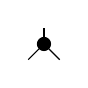
\begin{tikzpicture}[scale=0.2, black/.style={scale=0.5,draw,shape=circle,fill=black}]
	\node[black] (0) at (0, 0) {};
	\draw (1,-1) to (0);
	\draw (-1,-1) to (0);
	\draw (0) to (0,1);
	\end{tikzpicture}
}
\newcommand{\unit}{
	
\begin{tikzpicture}[scale=0.2, black/.style={scale=0.5,draw,shape=circle,fill=black}]
	\node[black] (0) at (0, 0) {};
	\draw (0) to (0,1);
	\end{tikzpicture}
}
\newcommand{\comult}{
	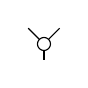
\begin{tikzpicture}[scale=0.2, black/.style={scale=0.5,draw,shape=circle,fill=white}]
	\node[black] (0) at (0, 0) {};
	\draw (1,1) to (0);
	\draw (-1,1) to (0);
	\draw (0) to (0,-1);
	\end{tikzpicture}
}

\newcommand{\counit}{
	\begin{tikzpicture}[scale=0.2, black/.style={scale=0.5,draw,shape=circle,fill=white}]
	\node[black] (0) at (0, 0) {};
	\draw (0) to (0,-1);
	\end{tikzpicture}
}

\newcommand{\antipode}{
	\begin{tikzpicture}[scale=0.2, black/.style={scale=0.5,draw,regular polygon,
		regular polygon sides=4,fill=white}]
	\node[scale=0.5, black] (0) at (0, 0) {$S$};
	\draw (0) to (0,-1);
	\draw (0) to (0,1);
	\end{tikzpicture}
}

\newcommand{\associativity}{
\begin{equation}
\begin{gathered}
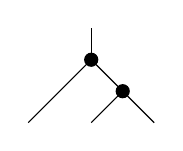
\begin{tikzpicture}[scale=0.8]
\node[scale=0.5,draw,circle,fill=black] (0) at (0,0.5) {};
\node[scale=0.5,draw,circle,fill=black] (1) at (0.5,0) {};
\draw (0) to (1);
\draw (-1,-0.5) to (0);
\draw (0,-0.5) to (1);
\draw (1,-0.5) to (1);
\draw (0) to (0,1);
\end{tikzpicture}
\end{gathered}
\, = \,
\begin{gathered}
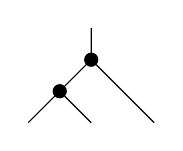
\begin{tikzpicture}[scale=0.8]
\node[scale=0.5,draw,circle,fill=black] (0) at (0.5,0.5) {};
\node[scale=0.5,draw,circle,fill=black] (1) at (0,0) {};
\draw (0) to (1);
\draw (-0.5,-0.5) to (1);
\draw (0.5,-0.5) to (1);
\draw (1.5,-0.5) to (0);
\draw (0) to (0.5,1);
\end{tikzpicture}
\end{gathered}
\end{equation}
}
\newcommand{\unitlaw}{
\begin{equation}\label{unitlaw}
\begin{gathered}
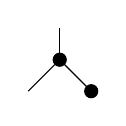
\begin{tikzpicture}[scale=0.8]
\node[scale=0.5,draw,circle,fill=black] (0) at (0,0.5) {};
\node[scale=0.5,draw,circle,fill=black] (1) at (0.5,0) {};
\draw (0) to (1);
\draw (-0.5,0) to (0);
\draw (0) to (0,1);
\end{tikzpicture}
\end{gathered}
\, = \,
\begin{gathered}
\begin{tikzpicture}[scale=0.8]
\draw (0,0) to (0,1);
\end{tikzpicture}
\end{gathered}
\, = \,
\begin{gathered}
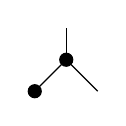
\begin{tikzpicture}[scale=0.8]
\node[scale=0.5,draw,circle,fill=black] (0) at (0,0.5) {};
\node[scale=0.5,draw,circle,fill=black] (1) at (-0.5,0) {};
\draw (0) to (1);
\draw (0.5,0) to (0);
\draw (0) to (0,1);
\end{tikzpicture}
\end{gathered}
\end{equation}
}
\newcommand{\coassociativity}{
\begin{equation}\label{coassociativity}
\begin{gathered}
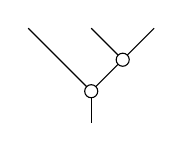
\begin{tikzpicture}[scale=0.8]
\node[scale=0.5,draw,circle,fill=white] (0) at (0,-0.5) {};
\node[scale=0.5,draw,circle,fill=white] (1) at (0.5,0) {};
\draw (0) to (1);
\draw (-1,0.5) to (0);
\draw (0,0.5) to (1);
\draw (1,0.5) to (1);
\draw (0) to (0,-1);
\end{tikzpicture}
\end{gathered}
\, = \,
\begin{gathered}
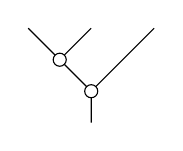
\begin{tikzpicture}[scale=0.8]
\node[scale=0.5,draw,circle,fill=white] (0) at (0.5,-0.5) {};
\node[scale=0.5,draw,circle,fill=white] (1) at (0,0) {};
\draw (0) to (1);
\draw (-0.5,0.5) to (1);
\draw (0.5,0.5) to (1);
\draw (1.5,0.5) to (0);
\draw (0) to (0.5,-1);
\end{tikzpicture}
\end{gathered}
\end{equation}
}
\newcommand{\counitlaw}{
\begin{equation}\label{counitlaw}
\begin{gathered}
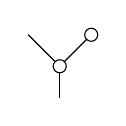
\begin{tikzpicture}[scale=0.8]
\node[scale=0.5,draw,circle,fill=white] (0) at (0,-0.5) {};
\node[scale=0.5,draw,circle,fill=white] (1) at (0.5,0) {};
\draw (0) to (1);
\draw (-0.5,0) to (0);
\draw (0) to (0,-1);
\end{tikzpicture}
\end{gathered}
\, = \,
\begin{gathered}
\begin{tikzpicture}[scale=0.8]
\draw (0,0) to (0,1);
\end{tikzpicture}
\end{gathered}
\, = \,
\begin{gathered}
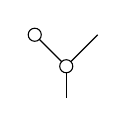
\begin{tikzpicture}[scale=0.8]
\node[scale=0.5,draw,circle,fill=white] (0) at (0,-0.5) {};
\node[scale=0.5,draw,circle,fill=white] (1) at (-0.5,0) {};
\draw (0) to (1);
\draw (0.5,0) to (0);
\draw (0) to (0,-1);
\end{tikzpicture}
\end{gathered}
\end{equation}
}

\newcommand{\bialgebralaw}{
\begin{equation}\label{bialgebralaw}
\begin{gathered}
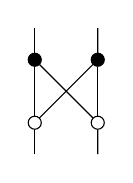
\begin{tikzpicture}[scale=0.8]
\node[scale=0.5,draw,circle,fill=white] (0) at (0,0) {};
\node[scale=0.5,draw,circle,fill=white] (1) at (1,0) {};
\node[scale=0.5,draw,circle,fill=black] (2) at (0,1) {};
\node[scale=0.5,draw,circle,fill=black] (3) at (1,1) {};
\draw (0) to (2);
\draw (0) to (3);
\draw (1) to (2);
\draw (1) to (3);
\draw (0,-0.5) to (0);
\draw (1,-0.5) to (1);
\draw (0,1.5) to (2);
\draw (1,1.5) to (3);
\end{tikzpicture}
\end{gathered}
\, = \,
\begin{gathered}
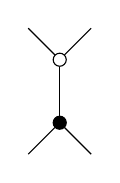
\begin{tikzpicture}[scale=0.8]
\node[scale=0.5,draw,circle,fill=black] (0) at (0.5,0) {};
\node[scale=0.5,draw,circle,fill=white] (1) at (0.5,1) {};
\draw (0) to (1);
\draw (0,-0.5) to (0);
\draw (1,-0.5) to (0);
\draw (0,1.5) to (1);
\draw (1,1.5) to (1);
\end{tikzpicture}
\end{gathered}
\end{equation}
}
\newcommand{\copylaw}{
\begin{equation}\label{copylaw}
\begin{gathered}
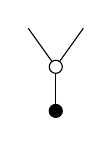
\begin{tikzpicture}[scale=0.7, squr/.style={scale=0.5,draw,regular polygon,
	regular polygon sides=4,fill=white}, black/.style={scale=0.5,draw,shape=circle,fill=black}, whit/.style={scale=0.5,draw,shape=circle,fill=white}]
\node[black] (0) at (0, 0) {};
\node[whit] (1) at  (0, 0.8) {};
\draw (0) to (1);
\draw (1) to (0.5,1.5);
\draw (1) to (-0.5,1.5);
\end{tikzpicture}
\end{gathered}
\, = \,
\begin{gathered}
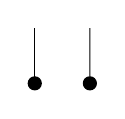
\begin{tikzpicture}[scale=0.7, black/.style={scale=0.5,draw,shape=circle,fill=black}]
\node[black] (0) at (0,0) {};
\node[black] (1) at (1,0) {};
\draw (0) to (0,1);
\draw (1) to (1,1);
\end{tikzpicture}
\end{gathered}
\end{equation}
}
\newcommand{\cocopylaw}{
	\begin{equation}\label{cocopylaw}
	\begin{gathered}
	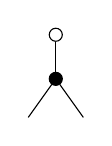
\begin{tikzpicture}[scale=0.7, squr/.style={scale=0.5,draw,regular polygon,
		regular polygon sides=4,fill=white}, black/.style={scale=0.5,draw,shape=circle,fill=black}, whit/.style={scale=0.5,draw,shape=circle,fill=white}]
	\node[whit] (0) at (0, 0) {};
	\node[black] (1) at  (0, -0.8) {};
	\draw (0) to (1);
	\draw (1) to (0.5,-1.5);
	\draw (1) to (-0.5,-1.5);
	\end{tikzpicture}
	\end{gathered}
	\, = \,
	\begin{gathered}
	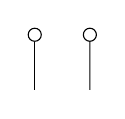
\begin{tikzpicture}[scale=0.7, black/.style={scale=0.5,draw,shape=circle,fill=white}]
	\node[black] (0) at (0,0) {};
	\node[black] (1) at (1,0) {};
	\draw (0) to (0,-1);
	\draw (1) to (1,-1);
	\end{tikzpicture}
	\end{gathered}
	\end{equation}
}
\newcommand{\hopflaw}{
	\begin{equation}\label{hopflaw}
	\begin{gathered}
	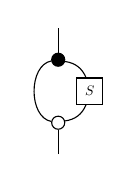
\begin{tikzpicture}[scale=0.8, squr/.style={scale=0.5,draw,regular polygon,
		regular polygon sides=4,fill=white}]
	\node[scale=0.5,draw,circle,fill=white] (0) at (0,0) {};
	\node[scale=0.5,draw,circle,fill=black] (1) at (0,1) {};
	\node[squr] (2) at (0.5,0.5) {$S$};
	\draw[bend left=80] (0) to (1);
	\draw[bend right] (0) to (2);
	\draw[bend right] (2) to (1);
	\draw (0,-0.5) to (0);
	\draw (0,1.5) to (1);
	\end{tikzpicture}
	\end{gathered}
	\, = \,
	\begin{gathered}
	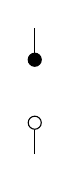
\begin{tikzpicture}[scale=0.8, squr/.style={draw,regular polygon,
		regular polygon sides=4,fill=white}]
	\node[scale=0.5,draw,circle,fill=white] (0) at (0,0) {};
	\node[scale=0.5,draw,circle,fill=black] (1) at (0,1) {};
	\draw (0,-0.5) to (0);
	\draw (0,1.5) to (1);
	\end{tikzpicture}
	\end{gathered}
	\, = \,
	\begin{gathered}
	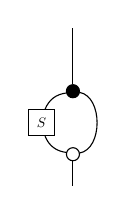
\begin{tikzpicture}[scale=0.8, squr/.style={scale=0.5,draw,regular polygon,
		regular polygon sides=4,fill=white}]
	\node[scale=0.5,draw,circle,fill=white] (0) at (0,0) {};
	\node[scale=0.5,draw,circle,fill=black] (1) at (0,1) {};
	\node[squr] (2) at (-0.5,0.5) {$S$};
	\draw[bend right=80] (0) to (1);
	\draw[bend left] (0) to (2);
	\draw[bend left] (2) to (1);
	\draw (0,-0.5) to (0);
	\draw (0,2) to (1);
	\end{tikzpicture}
	\end{gathered}
	\end{equation}
}
\newcommand{\skewhopflaw}{
	\begin{equation}\label{skewhopflaw}
	\begin{gathered}
	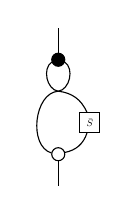
\begin{tikzpicture}[scale=0.8, squr/.style={scale=0.5,draw,regular polygon,
		regular polygon sides=4,fill=white}]
	\node[scale=0.5,draw,circle,fill=white] (0) at (0,0) {};
	\node[scale=0.5,draw,circle,fill=black] (1) at (0,1.5) {};
	\node[squr,scale=0.7] (2) at (0.5,0.5) {$\bar{S}$};
	\draw[bend left=80] (0) to (0,1);
	\draw[bend right=70] (0,1) to (1);
	\draw[bend right] (0) to (2);
	\draw[bend right] (2) to (0,1);
	\draw[bend left=70] (0,1) to (1);
	\draw (0,-0.5) to (0);
	\draw (0,2) to (1);
	\end{tikzpicture}
	\end{gathered}
	\, = \,
	\begin{gathered}
	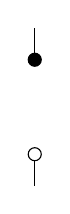
\begin{tikzpicture}[scale=0.8, squr/.style={draw,regular polygon,
		regular polygon sides=4,fill=white}]
	\node[scale=0.5,draw,circle,fill=white] (0) at (0,0) {};
	\node[scale=0.5,draw,circle,fill=black] (1) at (0,1.5) {};
	\draw (0,-0.5) to (0);
	\draw (0,2) to (1);
	\end{tikzpicture}
	\end{gathered}
	\, = \,
	\begin{gathered}
	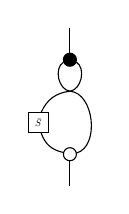
\begin{tikzpicture}[scale=0.8, squr/.style={scale=0.5,draw,regular polygon,
		regular polygon sides=4,fill=white}]
	\node[scale=0.5,draw,circle,fill=white] (0) at (0,0) {};
	\node[scale=0.5,draw,circle,fill=black] (1) at (0,1.5) {};
	\node[squr,scale=0.7] (2) at (-0.5,0.5) {$\bar{S}$};
	\draw[bend right=80] (0) to (0,1);
	\draw[bend left=70] (0,1) to (1);
	\draw[bend left] (0) to (2);
	\draw[bend left] (2) to (0,1);
	\draw[bend right=70] (0,1) to (1);
	\draw (0,-0.5) to (0);
	\draw (0,2) to (1);
	\end{tikzpicture}
	\end{gathered}
	\end{equation}
}
\newcommand{\modulelaw}{
	\begin{equation}\label{modulelaw}
	\begin{gathered}
	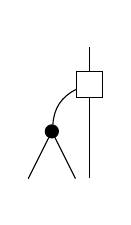
\begin{tikzpicture}[scale=0.6, squr/.style={draw,regular polygon,
		regular polygon sides=4,fill=white}, black/.style={scale=0.5,draw,shape=circle,fill=black}]
	\node (0) at (0, -2.2) {};
	\node[squr] (1) at (0, 0) {};
	\node (2) at (0, 1) {};
	\node[black] (3) at (-0.8, -1) {};
	\draw (0) to (1);
	\draw (1) to (2);
	\draw[bend left] (3) to (1);
	\draw (-1.3, -2) to (3);
	\draw (-0.3, -2) to (3);
	\end{tikzpicture}
	\end{gathered}
	\, = \,
	\begin{gathered}
	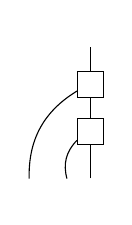
\begin{tikzpicture}[scale=0.6, squr/.style={draw,regular polygon,
		regular polygon sides=4,fill=white}, black/.style={draw,shape=circle,fill=black}]
	\node (0) at (0, -2.2) {};
	\node[squr] (1) at (0, 0) {};
	\node (2) at (0, 1) {};
	\node[squr] (3) at (0, -1) {};
	\draw (0) to (3);
	\draw (3) to (1);
	\draw (1) to (2);
	\draw (3) to (1);
	\draw[bend left] (-1.3, -2) to (1);
	\draw[bend left] (-0.5, -2) to (3);
	\end{tikzpicture}
	\end{gathered}
	\end{equation}
}
\newcommand{\comodulelaw}{
	\begin{equation}\label{comodulelaw}
	\begin{gathered}
	\begin{tikzpicture}[scale=0.6, squr/.style={draw,regular polygon,
		regular polygon sides=4,fill=white}, black/.style={scale=0.5,draw,shape=circle,fill=white}]
	\node (0) at (0, 2.2) {};
	\node[squr] (1) at (0, 0) {};
	\node (2) at (0, -2) {};
	\node[black] (3) at (-0.8, 1) {};
	\draw (0) to (1);
	\draw (1) to (2);
	\draw[bend right] (3) to (1);
	\draw (-1.3, 2) to (3);
	\draw (-0.3, 2) to (3);
	\end{tikzpicture}
	\end{gathered}
	\, = \,
	\begin{gathered}
	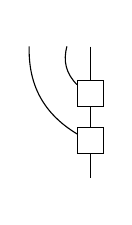
\begin{tikzpicture}[scale=0.6, squr/.style={draw,regular polygon,
		regular polygon sides=4,fill=white}, black/.style={draw,shape=circle,fill=black}]
	\node (0) at (0, 2.2) {};
	\node[squr] (1) at (0, 0) {};
	\node (2) at (0, -1) {};
	\node[squr] (3) at (0, 1) {};
	\draw (0) to (3);
	\draw (3) to (1);
	\draw (1) to (2);
	\draw (3) to (1);
	\draw[bend right] (-1.3, 2) to (1);
	\draw[bend right] (-0.5, 2) to (3);
	\end{tikzpicture}
	\end{gathered}
	\end{equation}
}
\newcommand{\intertwinerlaw}{
\begin{equation}
\begin{gathered}
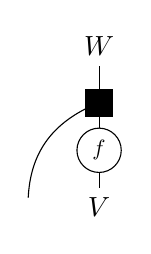
\begin{tikzpicture}[scale=0.6, squr/.style={draw,regular polygon,
	regular polygon sides=4,fill=black}]
\node (0) at (0, -2.2) {$V$};
\node[squr] (1) at (0, 0) {};
\node (2) at (0, 1.2) {$W$};
\node[scale=0.8,draw,circle] (3) at (0, -1) {$f$};
\draw (0) to (3);
\draw (3) to (1);
\draw (1) to (2);
\draw (3) to (1);
\draw[bend left] (-1.5, -2) to (1);
\end{tikzpicture}	
\end{gathered}
\, = \,
\begin{gathered}
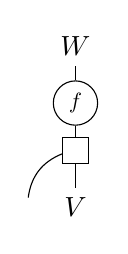
\begin{tikzpicture}[scale=0.6, squr/.style={draw,regular polygon,
	regular polygon sides=4,fill=white}]
\node (0) at (0, -2.2) {$V$};
\node[scale=0.8,draw,circle] (1) at (0, 0) {$f$};
\node (2) at (0, 1.2) {$W$};
\node[squr] (3) at (0, -1) {};
\draw (0) to (3);
\draw (3) to (1);
\draw (1) to (2);
\draw (3) to (1);
\draw[bend left] (-1, -2) to (3);
\end{tikzpicture}	
\end{gathered}
\end{equation}
}
\newcommand{\symAB}{
	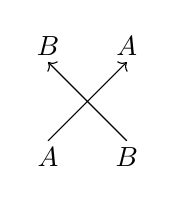
\begin{tikzpicture}[decoration={markings,mark=at position 0.5 with {\arrow{>}}}]
	\node (0) at (-0.5, -0.7) {$A$};
	\node (0) at (-0.5, 0.7) {$B$};
	\node (1) at (0.5, -0.7) {$B$};
	\node (1) at (0.5, 0.7) {$A$};
	\draw [->] (-0.5, -0.5) to (0.5, 0.5);
	\draw [->] (0.5, -0.5) to (-0.5, 0.5);
	\end{tikzpicture}
}

\newcommand{\symequation}{
	\begin{equation*}
	\begin{gathered}
	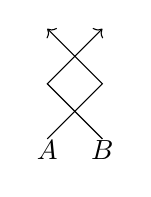
\begin{tikzpicture}[scale=0.7]
	\node (0) at (-1, -1.2) {$A$};
	\node (0) at (0, -1.2) {$B$};
	\draw [->] (-1, -1)--(0,0)--(-1,1);
	\draw [->] (0, -1)--(-1,0)--(0,1);
	\end{tikzpicture}
	\end{gathered}
	\, = \,
	\begin{gathered}
	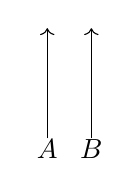
\begin{tikzpicture}[scale=0.7]
	\node (0) at (-0.8, -1.2) {$A$};
	\node (0) at (0, -1.2) {$B$};
	\draw [->] (-0.8, -1)--(-0.8,1);
	\draw [->] (0, -1)--(0,1);
	\end{tikzpicture}
	\end{gathered}
	\end{equation*}
}

\newcommand{\cupA}{	
	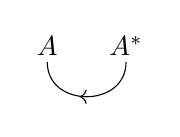
\begin{tikzpicture}[decoration={markings,mark=at position 0.5 with {\arrow{<}}}]
	\node (0) at (0, 0.2) {$A$};
	\node (1) at (1, 0.2) {$A^*$};
	\draw [bend right=90, looseness=1.5, postaction=decorate] (0,0) to (1,0);
	\end{tikzpicture}}

\newcommand{\capA}{	
	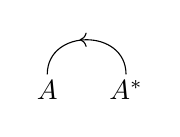
\begin{tikzpicture}[decoration={markings,mark=at position 0.5 with {\arrow{<}}}]
	\node (0) at (0, -0.2) {$A$};
	\node (1) at (1, -0.2) {$A^*$};
	\draw [bend left=90, looseness=1.5, postaction=decorate] (0,0) to (1,0);
	\end{tikzpicture}}

\newcommand{\snake}{
	\begin{equation*}
	\begin{gathered}
	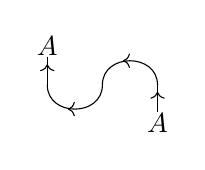
\begin{tikzpicture}[scale=0.7,decoration={markings,mark=at position 0.5 with {\arrow{<}}}]
	\node (0) at (0, 0.7) {$A$};
	\node (4) at (2, -0.7){$A$};
	\draw [bend right=90, looseness=1.5, postaction=decorate] (0, 0) to (1, 0);
	\draw [bend left=90, looseness=1.5, postaction=decorate] (1, 0) to (2, 0);
	\draw [postaction=decorate] (2, 0) to (2, -0.5);
	\draw [postaction=decorate] (0, 0.5) to (0, 0);
	\end{tikzpicture}
	\end{gathered}
	\, = \,
	\begin{gathered}
	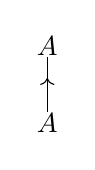
\begin{tikzpicture}[scale=0.7,decoration={markings,mark=at position 0.5 with {\arrow{<}}}]
	\node (0) at (0, 0.7) {$A$};
	\node (4) at (0, -0.7){$A$};
	\draw [postaction=decorate] (0, 0.5) to (0, -0.5);
	\end{tikzpicture}
	\end{gathered}
	\end{equation*}}

\newcommand{\snakestar}{
	\begin{equation*}
	\begin{gathered}
	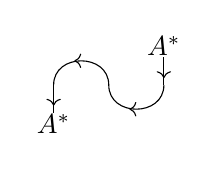
\begin{tikzpicture}[scale=0.7,decoration={markings,mark=at position 0.5 with {\arrow{<}}}]
	\node (0) at (0, -0.7) {$A^*$};
	\node (4) at (2, 0.7){$A^*$};
	\draw [bend left=90, looseness=1.5, postaction=decorate] (0, 0) to (1, 0);
	\draw [bend right=90, looseness=1.5, postaction=decorate] (1, 0) to (2, 0);
	\draw [postaction=decorate] (2, 0) to (2, 0.5);
	\draw [postaction=decorate] (0, -0.5) to (0, 0);
	\end{tikzpicture}
	\end{gathered}
	\, = \,
	\begin{gathered}
	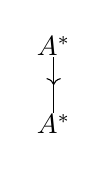
\begin{tikzpicture}[scale=0.7,decoration={markings,mark=at position 0.5 with {\arrow{>}}}]
	\node (0) at (0, 0.7) {$A^*$};
	\node (4) at (0, -0.7){$A^*$};
	\draw [postaction=decorate] (0, 0.5) to (0, -0.5);
	\end{tikzpicture}
	\end{gathered}
	\end{equation*}
}

\newcommand{\fusionijk}{
	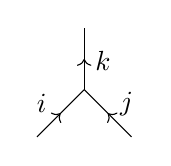
\begin{tikzpicture}[scale=0.6,decoration={markings,mark=at position 0.5 with {\arrow{>}}}]
	\node (0) at (-0.9, -0.3) {$i$};
	\node (1) at (0.9, -0.3) {$j$};
	\node (2) at (0.4, 0.6) {$k$};
	\draw [postaction=decorate] (-1, -1) to(0,0);
	\draw [postaction=decorate] (1,-1) to (0,0);
	\draw [postaction=decorate] (0,0) to (0,1.3);
	\end{tikzpicture}}
%%%%%%%%%%%%%%%%%%%%%%%%%%%%%%%%%%%%%%%%%%%%%%%%%%%%%%%%%%%%%%%%%%%%%%%%%%%%%%%%%%%%%%%%%%%%%%%%%%%%%%%%%%%%%%%%%%%%%%%%%%%%%%%%%%%%%%%%%%%%%%%%%%%%%%%%%%%%%%%%%%%%%%%%%%%%%%%%%%%%


\begin{document}
\maketitle
\tableofcontents

\pagebreak
\section{Introduction}
Algebraic structures have historically been described in set-theoretic terms. One usually considers a set equipped with functions satisfying certain axioms. For example, a monoid is a set equipped with a multiplication and a unit element satisfying associativity and the unit law. Category theory has first been introduced in 1971 by MacLane \cite{MacLane71} and provides a unifying framework for describing algebraic theories. Many of the driving notions of category theory arise through categorification of old set-theoretic notions \cite{Baez98}. Categorification is the process of replacing sets by categories, functions by functors and relaxing equations to natural isomorphisms between the functors. For example, the notion of a monoidal category is the categorification of that of a monoid. Since their preliminary study \cite{MacLane71} monoidal categories have been used as building blocks for more complex algebraic theories and have found many applications to quantum physics \cite{Abramsky04} \cite{Bartlett05} \cite{Vicary12} \cite{Rowell17}. They have a very intuitive two-dimensional diagrammatic language where algebraic equations are topological moves. Using this language it is possible to represent processes on physical systems \cite{Coecke17}, which can often be characterized by their symmetries. These latter are traditionally described by groups, as for instance for the symmetries of crystals \cite{Auslander65} or spin-$\frac{1}{2}$ particles \cite{Pauncz67}. Hopf algebras provide a generalization of group theory which allows describing the symmetries of many-body quantum systems as they treat local and global (or topological) symmetries on the same level \cite{Slingerland02}.\\
The aim of this thesis is to provide a diagrammatic treatment of Hopf algebras outlining their relationship to quantum computation.\\
In the first chapter we introduce monoidal categories to obtain a diagrammatic characterisation of Hopf Algebras as in [cite Sobocinski]. We then recall some standard results and move on to representation theory. Given a Hopf algebra $H$, the category of its representations $Rep(H)$ is monoidal and every object has a dual. If we additionally require $H$ to be quasitriangular, we obtain braids, making the language of $Rep(H)$ three dimensional. In these categories knots and links are endomorphisms of the unit object (i.e scalars), so that we naturally obtain topological invariants.\\
The second chapter is dedicated to the study of special types of particles called anyons. Their symmetries and exchange statistics are captured by quasitriangular Hopf algebras, so that categories of representations can be interpreted as process theories of anyons. We also see how the Drinfeld center construction, which takes place at the categorical level, corresponds to a certain quantization of the symmetries: the quantum double construction on a Hopf algebra.\\
In the last chapter we study two different models of quantum computation induced by Hopf algebras. 
Kitaev's double model for topological quantum computation (TQC) \cite{Kitaev03}, which is based on a group, is generalized to the Hopf algebra framework. 
Jordan's model for permutational quantum computing (PQC) \cite{Jordan09} is described from a categorical perspective in view of relating it to TQC. 
Finally, we project the pictures of knots from braided fusion categories into Hilbert spaces to obtain a braided syntax for quantum gates. 
%%%%%%%%%%%%%%%%%%%%%%%%%%%%%%%%%%%%%%%%%%%%%%%%%%%%%%%%%%%%%%%%%%%%%%%%%%%%%%%%%%%%%%%%%%%%%%%%%%%%%%%%%%%%%%%%%%%%%%%%%%%%%%%%%%%%%%%%%%%%%%%%
%%%%%%%%%%%%%%%%%%%%%%%%%%%%%%%%%%%%%%%%%%%%%%%%%%%%%%%%%%%%%%%%%%%%%%%%%%%%%%%%%%%%%%%%%%%%%%%%%%%%%%%%%%%%%%%%%%%%%%%%%%%%%%%%%%%%%%%%%%%%%%%%
%%%%%%%%%%%%%%%%%%%%%%%%%%%%%%%%%%%%%%%%%%%%%%%%%%%%%%%%%%%%%%%%%%%%%%%%%%%%%%%%%%%%%%%%%%%%%%%%%%%%%%%%%%%%%%%%%%%%%%%%%%%%%%%%%%%%%%%%%%%%%%%%
%%%%%%%%%%%%%%%%%%%%%%%%%%%%%%%%%%%%%%%%%%%%%%%%%%%%%%%%%%%%%%%%%%%%%%%%%%%%%%%%%%%%%%%%%%%%%%%%%%%%%%%%%%%%%%%%%%%%%%%%%%%%%%%%%%%%%%%%%%%%%%%%

\section{Diagrams and Hopf Algebras}\label{Diagramsandhopfalgebras}

\subsection{Monoidal categories}\label{Monoidalcategories}
In this section, we set in place the basic definitions and the diagrammatic framework which we will use throughout the thesis. The standard reference about basic category theory is \cite{MacLane71}. Many of the definitions are taken from \cite{Abramsky11}. For an introduction to diagrammatic reasoning in monoidal categories consider the first two chapters of \cite{Coecke17}. A more technical and up to date survey on monoidal categories can be found in \cite{Etingof15}. Many of the results recalled in this section and their relationship to quantum mechanics can be found in \cite{Vicary12}.
\begin{definition}[Category]
	A category $\cat$ consists of the data:
	\begin{itemize}
		\item a collection of objects $obj(\cat)$,
		\item a collection of morphisms (or arrows) $arr(\cat)$,
		\item domain and codomain assignments: $dom, cod: arr(\cat) \rightarrow obj(\cat)$. For any two objects $a,b \in obj(\cat)$ we define the hom-set 
		$$ \cat (a,b) := \{ f \in arr(\cat) : a= dom(f), b=cod(f) \}$$
		\item for any triple of objects $a$,$b$ and $c$, a composition map 
		$$ \cat (a,b) \times \cat (b,c) \rightarrow \cat (a,c)$$
		we denote the composition by $g \circ f$, diagrammatically:
		\begin{center}
			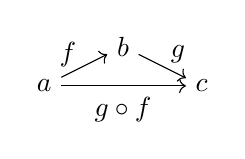
\begin{tikzpicture}
			\node (0) at (-1, 0) {$a$};
			\node (1) at (0, 0.5) {$b$};
			\node (2) at (1, 0) {$c$};
			\node (3) at (-0.7, 0.4) {$f$};
			\node (3) at (0.7, 0.4) {$g$};
			\node (3) at (0, -0.3) {$g\circ f$};
			\draw [->] (0) to (1);
			\draw [->] (1) to (2);
			\draw [->] (0) to (2);
			\end{tikzpicture}
		\end{center}
		\item For any object $a$ an identity morphism $id_a: a \rightarrow a$. 
	\end{itemize}
	Satisfying the following axioms:
	\begin{equation*}
		h \circ (g \circ f) = (h \circ g) \circ f \quad; \quad f \circ id_a = f = id_b \circ f
	\end{equation*}	
\end{definition}
\begin{example}
	Examples of categories are: $Sets$ of sets and functions, $FSets$ of finite sets and functions, $Rel$ of sets and relations, $Vect_k$ of vector spaces over a field $k$ and linear maps and $FVect_k$ of finite dimensional vector spaces and linear maps.
\end{example}
Category theory expresses equivalences and relationships between structures by means of the following tools.
\begin{definition}[Functor]
	A functor $F:\mathcal{C} \rightarrow \mathcal{D}$ is a mapping that
	\begin{itemize}
		\item associates an object $F(a)$ of $\mathcal{D}$ to each object $a$ of $\mathcal{C}$,
		\item associates to each morphism $f: a \rightarrow b$ in $\cat$ a morphism $F(f): F(a) \rightarrow F(b)$ in $\mathcal{D}$ such that $F(id_a)=id_{F(a)}$ and $F(g\circ f)= F(g)\circ F(f)$ for all morphisms $f:a \rightarrow b$ and $g:b \rightarrow c$.
	\end{itemize}
\end{definition}
For instance, there is a functor $Q: FSets \rightarrow FVect_k$ (which we will call `1st quantization') taking a set to the free vector space generated by that set.
Given two functors with matching source and target we can have natural transformations between them.
\begin{definition}[Natural Transformation]
	Given categories $\cat$ and $\mathcal{D}$ and functors $F,G:\cat \rightarrow \mathcal{D}$ a natural transformation $\alpha: F \Rightarrow G$ is an assignment to every object $a$ in $\cat$ of a morphism $\alpha_a:F(a) \rightarrow G(a)$ in $\mathcal{D}$ such that for each morphism $f:a \rightarrow b$, the following commutes:
	\begin{center}
		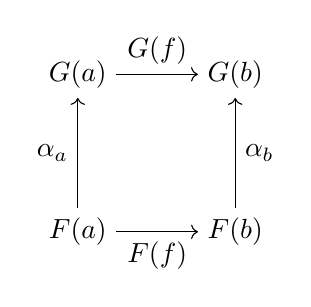
\begin{tikzpicture}[scale=2]
		\node (0) at (0,0) {$F(a)$};
		\node (1) at (0,1) {$G(a)$};
		\node (3) at (1,0) {$F(b)$};
		\node (4) at (1,1) {$G(b)$};
		\draw [->] (0)--(1) node[midway,left] {$\alpha_a$};
		\draw [->] (3)--(4) node[midway,right] {$\alpha_b$};
		\draw [->] (0)--(3) node[midway,below] {$F(f)$};
		\draw [->] (1)--(4) node[midway,above] {$G(f)$};
		\end{tikzpicture}
	\end{center}
	A natural isomorphism is a natural transformation such that all components are isomorphisms.
\end{definition}
%%%MONOIDAL CATEGORIES:
Recall that a monoid is a triple $(X, \times, 1)$ where $X$ is a set, $1 \in X$ and $\times$ is an associative and unital multiplication on $X$. The notion of a monoidal category is the categorification of a monoid. Elements of the set are replaced by objects in a category $\mathcal{C}$, multiplication by a functor $\otimes: \mathcal{C} \times \mathcal{C} \rightarrow \mathcal{C}$ and the equalities in the unit and association axioms are replaced by natural isomorphisms. In order for this new structure to be well-behaved we will also need to impose compatibility conditions. We obtain the following definition:
\begin{definition}[Monoidal category]
A monoidal category is a category $\mathcal{C}$ equipped with a functor $\otimes: \mathcal{C} \times \mathcal{C} \rightarrow \mathcal{C}$ called tensor product, an object $1$ called unit object, a natural isomorphism
$$ \alpha : (-\otimes -) \otimes - \xRightarrow{\sim} -\otimes (- \otimes -)$$ 
called associator, a natural isomorphism 
$$\lambda: 1 \otimes (-) \xRightarrow{\sim} (-)$$ called left unitor and a natural isomorphism
$$ \rho: (-) \otimes 1 \xRightarrow{\sim} (-)$$
called right unitor. Subject to the following coherence conditions holding for all objects $a,b,c,d$ in $\mathcal{C}$:
\begin{enumerate}
    \item Pentagon axiom: the following diagram commutes
    \begin{center}
    	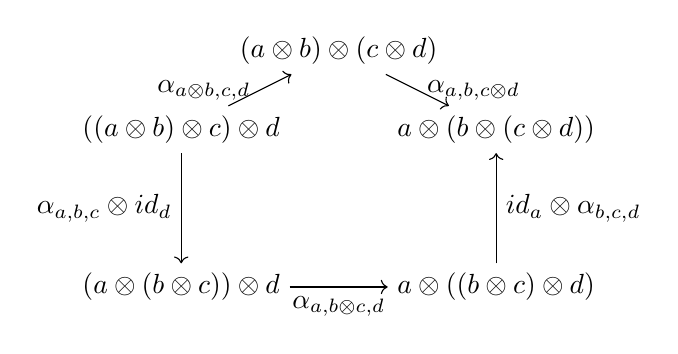
\begin{tikzpicture}[scale=2]
    	\node (0) at (0,0) {$(a\otimes (b \otimes c)) \otimes d$};
    	\node (1) at (0,1) {$((a\otimes b) \otimes c) \otimes d$};
    	\node (2) at (1,1.5) {$(a\otimes b) \otimes (c \otimes d)$};
    	\node (3) at (2,1) {$a\otimes (b \otimes (c \otimes d))$};
    	\node (4) at (2,0) {$a\otimes ((b \otimes c) \otimes d)$};
    	\draw [->] (1)--(2) node[midway,left] {$\alpha_{a \otimes b,c,d}$};
    	\draw [->] (2)--(3) node[midway,right] {$\alpha_{a, b,c \otimes d}$};
    	\draw [->] (1)--(0) node[midway,left] {$\alpha_{a, b,c} \otimes id_d$};
    	\draw [->] (0)--(4) node[midway,below] {$\alpha_{a,b \otimes c,d}$};
    	\draw [->] (4)--(3) node[midway,right] {$id_a \otimes \alpha_{b,c,d}$};
    	\end{tikzpicture}
    \end{center}
    \item Triangle identity: the following diagram commutes
    \begin{center}
    	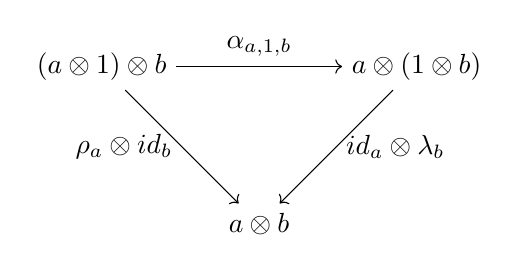
\begin{tikzpicture}[scale=2]
    	\node (0) at (0,0) {$(a\otimes 1) \otimes b$};
    	\node (1) at (2,0) {$a\otimes (1 \otimes b)$};
    	\node (2) at (1,-1) {$a\otimes b$};
    	\draw [->] (0)--(1) node[midway,above] {$\alpha_{a ,1,b}$};
    	\draw [->] (1)--(2) node[midway,right] {$id_a \otimes \lambda_b$};
    	\draw [->] (0)--(2) node[midway,left] {$\rho_a \otimes id_b$};
    	\end{tikzpicture}
    \end{center}
\end{enumerate}
\end{definition}
\begin{example}
The category $Sets$ of sets and functions is monoidal with the cartesian product $\times$ and the singleton set as unit object.\\
The category $Vect_k$ of finite dimensional vector spaces over a field $k$ is monoidal with the usual tensor product $\otimes$ and the one dimensional vector space $k$ as unit object.\\
The category $Rel$ of sets and relations is monoidal with the cartesian product $\times$ and the singleton as unit object.\\
The category $Hilb$ of Hilbert spaces and linear maps is monoidal when equipped with the usual tensor product $\otimes$.
\end{example}
The pentagon and triangle axioms make sure that any well formed diagram in a monoidal category, made up of associators and unitors, commutes. This is known as the coherence theorem for monoidal categories and can be found in \cite{MacLane71}. When the associators and unitors are trivial morphisms (i.e identity morphisms) we say the category is strict monoidal. It is known that every monoidal category is equivalent to a strict one \cite{MacLane71}, but it is sometimes useful to take associators into account as we will see in our discussion on permutational quantum computation. Strict monoidal categories have a two-dimensional diagrammatic language which is rigorous \cite{Vicary12}. Objects are represented by their identity morphisms which we draw as labelled wires:
\begin{center}
	\begin{tikzpicture}[scale=0.7]
	\node (0) at (-0.4, 1) {$a$};
	\draw[->] (0,0)--(0,2);
	\end{tikzpicture}
\end{center}
A morphism $f:a \rightarrow c$ is drawn as a box with input and output wires going from bottom to top:
\begin{center}
	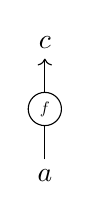
\begin{tikzpicture}[scale=0.7]
	\node (0) at (0, -1.2) {$a$};
	\node (2) at (0, 1.2) {$c$};
	\node[scale=0.6,draw,circle] (5) at (0, 0) {$f$};
	\draw[->] (0)--(5)--(2);
	\end{tikzpicture}
\end{center}
The vertical composition $h\circ f$ where $h:c \rightarrow e$ is denoted as:
\begin{center}
	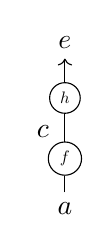
\begin{tikzpicture}[scale=0.7]
	\node (0) at (0, -1.2) {$a$};
	\node (1) at (-0.4, 0.2) {$c$};
	\node (2) at (0, 1.8) {$e$};
	\node[scale=0.6,draw,circle] (5) at (0, -0.3) {$f$};
	\node[scale=0.6,draw,circle] (6) at (0, 0.8) {$h$};
	\draw[->] (0)--(5)--(6)--(2);
	\end{tikzpicture}
\end{center}
We write the tensor of two morphisms $f \otimes g : a \otimes b \rightarrow c \otimes d$ simply putting them side by side:
\begin{center}
	\begin{tikzpicture}[scale=0.7]
	\node (0) at (0, -1.2) {$a$};
	\node (1) at (1, -1.2) {$b$};
	\node (2) at (0, 1.2) {$c$};
	\node (3) at (1, 1.2) {$d$};
	\node[scale=0.7,draw,circle] (5) at (0, 0) {$f$};
	\node[scale=0.7,draw,circle] (6) at (1, 0) {$g$};
	\draw (0) to (5);
	\draw [->] (5) to (2);
	\draw (1) to (6);
	\draw [->] (6) to (3);
	\end{tikzpicture}
\end{center}
Note that because the category is strict $id_1 \otimes f = f = f \otimes id_1$ for any $f$, so we could draw as many copies as we like of $id_1$ on any diagram to obtain an equivalent one. So really the identity on $1$ is just the empty diagram which we can stick next to any diagram we like.
\begin{definition}[States and costates]
	Given a system $A$, a state of $A$ is a morphism $y:1 \rightarrow a$. A costate (or effect) of $a$ is a morphism $x:a \rightarrow 1$. In the diagrammatic language we draw states and costates respectively:
	\begin{center}
		\begin{tikzpicture}[scale=0.7]
		\node[scale=0.5,buffer] (1) {$y$}; 
		\node (2) at (0.3,0.7) {$a$};
		\draw (1)--(0,1);
		\end{tikzpicture}
		\quad \quad \quad
		\begin{tikzpicture}[scale=0.7]
		\node[scale=0.5,buffer,rotate=180] (1) at (0,0) {$x$}; 
		\node (2) at (0.3,-0.7) {$a$};
		\draw (1)--(0,-1);
		\end{tikzpicture}
	\end{center}
\end{definition}
\begin{example}
The cartesian product $\times$ in $Sets$ satisfies the universal properties of a categorical product, in the sense that we have projections $p_1: A \times B \rightarrow A$ and $p_2: A \times B \rightarrow B$  such that if $f$ and $g$ are maps from some set $C$ there is a unique function $h$ making the following diagram commute:
\begin{center}
	\begin{tikzpicture}
	\node (0) at (-1, 0) {$A$};
	\node (1) at (1, 0) {$B$};
	\node (2) at (0, 1) {$A \times B$};
	\node (3) at (0, -1) {$C$};
	\node (4) at (0.2, 0) {$h$};
	\node (5) at (-0.8, 0.6) {$p_1$};
	\node (6) at (0.8, 0.6) {$p_2$};
	\node (7) at (-0.8, -0.6) {$f$};
	\node (8) at (0.8, -0.6) {$g$};
	\draw [->] (2) to (0);
	\draw [->] (2) to (1);
	\draw [->] (3) to (1);
	\draw [->] (3) to (0);
	\draw [->] (3) to (2);
	\end{tikzpicture}
\end{center}
This implies that all states in $(Sets, \times)$ are separable, in the sense that any state $c$ of $A \times B$ is a product state $a \times b$. $Sets$ is the ambient Cartesian world of classical physics.
\end{example}
\begin{example}
In $Vect_k$ states are vectors and costates are functionals. Note that the diagrammatic notation provides a two-dimensional generalisation of Dirac's notation. Note that the tensor of vector spaces $\otimes$ is not a categorical product, and in fact we can have entangled states.
\end{example}
\begin{definition}[Scalars]
Scalars in a monoidal category are morphisms $1 \rightarrow 1$.
\end{definition}
The category $Sets$ has only one scalar. $Rel$ has two scalars forming the booleans $\mathbb{B}_2$ under composition. $Vect_k$ has scalars from $k$. Given a vector and a functional we obtain a scalar by composing them analogously to Dirac's formalism.
\begin{definition}[BMC]
	A braided monoidal category is a monoidal category $\mathcal{C}$ equipped with a natural isomorphism $B_{a,b} : a \otimes b \rightarrow b \otimes a$ called braiding, subject to the following compatibility conditions (called hexagon equations):
	\begin{center}
		\begin{tikzpicture}[scale=2]
		\node (0) at (-1,0) {$(a\otimes b) \otimes c$};
		\node (1) at (-0.5,1) {$a\otimes (b \otimes c)$};
		\node (2) at (1.5,1) {$(b\otimes c)\otimes a$};
		\node (3) at (2,0) {$b\otimes (c\otimes a)$};
		\node (4) at (-0.5,-1) {$(b\otimes a)\otimes c$};
		\node (5) at (1.5,-1) {$b\otimes (a\otimes c)$};
		\draw [->] (0)--(1) node[midway,left] {$\alpha_{a,b,c}$};
		\draw [->] (1)--(2) node[midway,above] {$B_{a,b \otimes c}$};
		\draw [->] (2)--(3) node[midway,right] {$\alpha_{b,c,a}$};
		\draw [->] (0)--(4) node[midway,left] {$B_{a,b} \otimes id_c$};
		\draw [->] (4)--(5) node[midway,below] {$\alpha_{b,a,c}$};
		\draw [->] (5)--(3) node[midway,right] {$id_b \otimes B_{a,c}$};
		\end{tikzpicture}
	\end{center}
	\begin{center}
		\begin{tikzpicture}[scale=2]
		\node (0) at (-1,0) {$a\otimes (b \otimes c)$};
		\node (1) at (-0.5,1) {$(a\otimes b) \otimes c$};
		\node (2) at (1.5,1) {$c\otimes (a\otimes b)$};
		\node (3) at (2,0) {$(c\otimes a)\otimes b$};
		\node (4) at (-0.5,-1) {$a\otimes (c\otimes b)$};
		\node (5) at (1.5,-1) {$(a\otimes c)\otimes b$};
		\draw [->] (0)--(1) node[midway,left] {$\alpha_{a,b,c}$};
		\draw [->] (1)--(2) node[midway,above] {$B_{a\otimes b,c}$};
		\draw [->] (2)--(3) node[midway,right] {$\alpha_{c,a,b}$};
		\draw [->] (0)--(4) node[midway,left] {$id_a \otimes B_{b,c}$};
		\draw [->] (4)--(5) node[midway,below] {$\alpha_{a,c,b}$};
		\draw [->] (5)--(3) node[midway,right] {$B_{a,c} \otimes id_b$};
		\end{tikzpicture}
	\end{center}
	
\end{definition}
In the diagrammatic language this means we have braidings:
\begin{center}
	\begin{tikzpicture}[scale=0.9, whit/.style={draw,regular polygon,
		regular polygon sides=4,fill=white}, black/.style={draw,regular polygon, regular polygon sides=4,fill=black}]
	\node (0) at (0.5,0.5) {};
	\node (1) at (-0.1,-0.4) {$A$};
	\node (2) at (1.1,-0.4) {$B$};
	\draw (0,1) to (1,0);
	\draw (0,0) to (0);
	\draw (0) to (1,1);
	\end{tikzpicture}
	\begin{tikzpicture}[scale=0.9, whit/.style={draw,regular polygon,
		regular polygon sides=4,fill=white}, black/.style={draw,regular polygon, regular polygon sides=4,fill=black}]
	\node (0) at (0.5,0.5) {};
	\node (1) at (-0.1,-0.4) {$B$};
	\node (2) at (1.1,-0.4) {$A$};
	\draw (0,0) to (1,1);
	\draw (0,1) to (0);
	\draw (0) to (1,0);
	\end{tikzpicture}
\end{center}
for any $A$ and $B$, satifying:
\begin{equation}
\begin{gathered}
\begin{tikzpicture}[scale=0.6, whit/.style={draw,regular polygon,
	regular polygon sides=4,fill=white}, black/.style={draw,regular polygon, regular polygon sides=4,fill=black}]
\node (0) at (0.5,0.5) {};
\node (1) at (-0.1,-0.4) {$A$};
\node (2) at (1.1,-0.4) {$B$};
\node (3) at (0.5,1.5) {};
\draw (1,0)--(0,1)--(1,2);
\draw (0,0)--(0)--(1,1)--(3)--(0,2);
\end{tikzpicture}
\end{gathered}
\, = \,
\begin{gathered}
\begin{tikzpicture}[scale=0.6, whit/.style={draw,regular polygon,
	regular polygon sides=4,fill=white}, black/.style={draw,regular polygon, regular polygon sides=4,fill=black}]
\node (1) at (0,-0.4) {$A$};
\node (2) at (0.9,-0.4) {$B$};
\draw (0.8,0)--(0.8,2);
\draw (0.1,0)--(0.1,2);
\end{tikzpicture}
\end{gathered}
\quad;\quad
\begin{gathered}
\begin{tikzpicture}[scale=0.6, whit/.style={draw,regular polygon,
	regular polygon sides=4,fill=white}, black/.style={draw,regular polygon, regular polygon sides=4,fill=black}]
\node (0) at (0.5,0.5) {};
\node (1) at (-0.1,-0.4) {$B$};
\node (2) at (1.1,-0.4) {$A$};
\node (3) at (0.5,1.5) {};
\draw (1,0)--(0)--(0,1)-- (3)--(1,2);
\draw (0,0)--(1,1)--(0,2);
\end{tikzpicture}
\end{gathered}
\, = \,
\begin{gathered}
\begin{tikzpicture}[scale=0.6, whit/.style={draw,regular polygon,
	regular polygon sides=4,fill=white}, black/.style={draw,regular polygon, regular polygon sides=4,fill=black}]
\node (1) at (0,-0.4) {$B$};
\node (2) at (0.9,-0.4) {$A$};
\draw (0.8,0)--(0.8,2);
\draw (0.1,0)--(0.1,2);
\end{tikzpicture}
\end{gathered}
\end{equation}
The compatibility conditions are obvious statements in the diagrammatic calculus, for instance the first hexagon equation just says:
\begin{equation}
\begin{gathered}
\begin{tikzpicture}[scale=0.6]
\node (0) at (0.5,0.5) {};
\node (1) at (-0.1,-0.4) {$A$};
\node (2) at (1.1,-0.4) {$B$};
\node (3) at (2.1,-0.4) {$C$};
\node (4) at (1.5,2.5) {};
\draw (0,0)--(1,1)--(1,2)--(2,3);
\draw (1,0)--(0)--(0,1)--(0,3);
\draw (2,0)--(2,2)--(4)--(1,3);
\end{tikzpicture}
\end{gathered}
\, = \,
\begin{gathered}
\begin{tikzpicture}[scale=0.6]
\node (0) at (1.3,2.2) {};
\node (1) at (0.4,-0.4) {$A$};
\node (2) at (1.5,-0.4) {$B$};
\node (3) at (2.2,-0.4) {$C$};
\node (4) at (1.5,2.5) {};
\draw (0.5,0)--(0.5,1.5)--(1,2)--(2,3);
\draw (1.7,0)--(1.7,1.7)--(0)--(0.5,3);
\draw (2,0)--(2,2)--(4)--(1,3);
\end{tikzpicture}
\end{gathered}
\end{equation}
Both $Sets$ and $Hilb$ are examples of symmetric monoidal categories in the following sense.
\begin{definition}[SMC]
	A braided monoidal category is symmetric if the braiding $B_{a,b}$ satisfies $$B_{a,b} \circ B_{b,a} = id_{a\otimes b}$$
	For all objects $a,b$
\end{definition}
In a SMC the braiding is called symmetry morphism and is denoted
\begin{center}
	\symAB	
\end{center}
It satisfies:
\symequation
We will now describe some new classes of examples of monoidal categories. These are of a different nature to the categories we have seen so far.
\begin{definition}[PROPs]
	A $PROP$ (products and permutations category) is a strict symmetric monoidal category where every object is of the form $x^{\otimes n}$ for a single object $x$ and $n \geq 0$.
\end{definition}
This means that we are only allowed one type of wire when drawing diagrams about $PROPs$ but we can use as many copies as we like and we can make swaps with them. Categories satisfying these properties are useful syntactic tools as we will see.
One way to think of a $PROP$ $A$ is as an abstract algebraic structure carrying some axioms, we can then instantiate those axioms in some other symmetric monoidal category $\mathcal{C}$ by considering symmetric monoidal functors $F: A \rightarrow \mathcal{C}$. We call such functors algebras or models of $A$ in $\mathcal{C}$. If $A$ is defined in terms of generators and relations (as is most often done), the choice of such functor corresponds to the choice of one object from $\mathcal{C}$ and morphisms on that object respecting the defining relations of $A$. On its own $A$ has no clear interpretation, it just defines a syntax, but if $\mathcal{C}$ is a semantic category (i.e one with a clear interpretation) then $F$ is a `filling' of the syntax with meaning. This reasoning was first proposed in Lawvere's Phd thesis in 1963 \cite{Lawvere63}.\\
It will sometimes be useful to drop the `permutational' structure of $PROPs$.
\begin{definition}[PRO]
	A $PRO$ (products category) is a strict monoidal category where every object is of the form $x^{\otimes n}$ for a single object $x$ and $n \geq 0$.
\end{definition}
The semantic categories we will consider the most are $Sets$ and $Hilb$. One important difference between them is that $Hilb$ exhibits duality.
\begin{definition}[Rigidity]
	Let $\mathcal{C}$ be a monoidal category and $A\in obj(\mathcal{C})$. A left-dual of $A$ is an object $A^*$ with morphisms
	\begin{center}
		\cupA \, \capA
	\end{center}
	Satisfying the snake equations:
	\snake
	\snakestar
	If every object has a left-dual, we say that $\mathcal{C}$ is left-rigid.
	Similarly we can define right-duals and right-rigid categories by interchanging the roles of $A$ and $A^\star$ in the definition.
\end{definition}
Given a (left/right) rigid structure we can define (left/right)transpose as follows.
\begin{definition}[Transpose]
	Given a (left/right) rigid category $\cat$ and any process $f:A \rightarrow B$ the (left/right) transpose $f^*$ (or left transpose $f^l$, right transpose $f^r$ if it is not clear from context) is:
	\begin{equation}
	\begin{gathered}
	\begin{tikzpicture}
		\node[draw, trapezium, trapezium angle=70, shape border rotate=180] (0) at (0,0) {$f$};
		\draw[->] (0) to (0,-0.7);
		\draw[->] (0,0.7) to (0);
	\end{tikzpicture}
	\end{gathered}
	\, = \,
	\begin{gathered}
	\begin{tikzpicture}
	\node[draw, trapezium, trapezium angle=70,] (0) at (0,0) {$f$};
	\draw[->] (0,-0.7)--(0)--(0,0.7);
	\draw[bend right=90] (0,0.7) to (-0.7,0.7);
	\draw[->] (-0.7,0.7) to (-0.7,-0.7);
	\draw[bend right=90] (0,-0.7) to (0.7,-0.7);
	\draw[->] (0.7,0.7) to (0.7,-0.7);
	\end{tikzpicture}
	\end{gathered}	
	\end{equation}
\end{definition}
\begin{definition}[Trace]
	In a symmetric monoidal category $\cat$, if $A$ has a left dual $A^\star$, the trace of some morphism $f:A \rightarrow A$ is defined as the following scalar:
	\begin{center}
	\begin{tikzpicture}[scale=0.7]
	\node[scale=0.7, draw, trapezium, trapezium angle=70,] (0) at (0,0) {$f$};
	\draw[->] (0,-0.7)--(0)--(0,0.7);
	\draw[bend right=90] (0,0.7) to (-0.7,0.7);
	\draw[->] (-0.7,0.7) to (-0.7,-0.7);
	\draw[bend left=90] (0,-1.3) to (-0.7,-1.3);
	\draw[->] (-0.7,-0.7) to (0,-1.3);
	\draw[->] (0,-0.7) to (-0.7,-1.3);
	\end{tikzpicture}	
	\end{center}
\end{definition}
A pivotal structure on a rigid monoidal category $\cat$ is a natural isomorphism $id_\cat \Rightarrow (-)^{\star \star}$. It allows to define traces without using the symmetry. Most categories we will consider have both sided duals, and therefore a trivial (identity) pivotal structure. Given a pivotal structure we can define left pivotal traces as:
\begin{center}
	\begin{tikzpicture}[scale=0.7]
	\node[scale=0.7, draw, trapezium, trapezium angle=70,] (0) at (0,0) {$f$};
	\draw[->] (0,-0.7)--(0)--(0,0.7);
	\draw[bend right=90] (0,0.7) to (-0.7,0.7);
	\draw[->] (-0.7,0.7) to (-0.7,-0.7);
	\draw[bend left=90] (0,-0.7) to (-0.7,-0.7);
	\end{tikzpicture}	
\end{center}
Where we have hidden the pivotal natural isomorphism. Similarly we can define right pivotal traces on endomorphisms in the obvious way.
\begin{definition}
	A rigid monoidal category with a pivotal strucutre is spherical if left and right traces coincide. In a spherical category, if $a$ is an object, the trace $tr: End(a) \rightarrow End(1)$ is well defined and $tr(id_a)$ is called the categorical (or quantum) dimension of $a$. 
\end{definition}
For a braided monoidal category, giving a spherical structure is equivalent to giving a ribbon structure \cite{Mueger12} where:
\begin{definition}
	A ribbon (or twist) structure on a braided monoidal category with left duality $\star$ is a natural isomorphism $\theta: id_\cat \Rightarrow id_\cat$ satisfying:
	\begin{equation}
	\begin{gathered}
	\begin{tikzpicture}
	\node[scale=0.7, draw, trapezium, trapezium angle=90] (0) at (0,0) {$\theta_{a \otimes b}$};
	\draw (0) to (-0.2,-1.5);
	\draw (-0.2,1) to (0);
	\draw (0) to (0.2,-1.5);
	\draw (0.2,1) to (0);
	\end{tikzpicture}
	\end{gathered}
	\, = \,
	\begin{gathered}
	\begin{tikzpicture}
	\node[scale=0.7, draw, trapezium, trapezium angle=90] (0) at (-0.3,0.5) {$\theta_{a}$};
	\node[scale=0.7, draw, trapezium, trapezium angle=90] (1) at (0.3,0.5) {$\theta_{b}$};
	\node (2) at (0,0) {};
	\node (3) at (0,-1) {};
	\draw (0) to (-0.3,1);
	\draw (1) to (0.3,1);
	\draw (0)--(0.3,-0.5)--(3)--(-0.3,-1.5);
	\draw (1)--(2)--(-0.3,-0.5)--(0.3,-1.5);
	\end{tikzpicture}
	\end{gathered}
	\end{equation}
	and compatible with the rigid structure $(\theta_a)^\star = \theta_{a^\star}$ 
\end{definition}
\begin{remark}
	It can be shown that in the diagrammatic language, having a ribbon structure really corresponds to replacing wires by ribbons which we can twist. We won't use such diagrammatic language, but in the section on modular categories the twist will be an important process.
\end{remark}

%%%%%%%%%%%%%%%%%%%%%%%%%%%%%%%%%%%%%%%%%%%%%%%%%%%%%%%%%%%%%%%%%%%%%%%%%%%%%%%%%%%%%%%%%%%%%%%%%%%%%%%%%%%%%%%%%%%%%%%%%%%%%%%%%%%%%%%%%%%%%%%%%%%%%%%%%%%%%%%%%%%%%%%%%%%%%%%%%%%%%%%%%%%%%%%%%%%%%%%%%%%%%%%%%%%%%%%%%%%%%%%%%%%%%%%%%%%%%%%%%%%%%%%%%%%%%%%%%%%%%%%%%%%%%%%%%%%%%%%%%%%%%%%%%%%%%%%%%%%%%%%%%%%%%%%%%%%%%%%%%%%%%%%%%%%%%%%%%%%%%%%%%%%%%%%%%%%%%%%%%%

\subsection{Hopf Algebras}\label{Hopfalgebras}
Now that we have set in place a diagrammatic machinery based on monoidal categories, let us make use of it. In this section we will meet some mathematical structures which have been used by mathematicians to describe symmetry. The notion of Hopf algebras is a powerful generalization of that of a group. Since their discovery in the 1940s, Hopf algebras have been used in various fields of pure mathematics (such as number theory, algebraic geometry, and representation theory) and have found applications in Quantum mechanics. Most of the results of this section can be found in \cite{Majid95}. 
\begin{definition}[Monoid]
	$\Delta$ is a $PRO$ generated by morphisms (\mult, \unit) satisfying associativity: \associativity
	and the unit law: \unitlaw
\end{definition}
Models of $\Delta$ in monoidal categories are called monoids and they are very well known, examples include the natural numbers under addition, lists of some alphabet under concatenation and any group. Taking the opposite category $\Delta^{op}$ corresponds to flipping all the diagrams.
\begin{definition}[Comonoid]
	$\Delta^{op}$ is a $PRO$ generated (\comult, \counit) satisfying coassociativity: \coassociativity and the counit law: \counitlaw
\end{definition}
Models of these are comonoids, the most common example is the copy map on any set with `delete' as counit.
Monoids and comonoids are simple structures that we can stick together to form more complicated ones. Bialgebras arise from one type of interaction of a monoid and comonoid.
\begin{definition}[Bialg]
	$Bialg$ is a $PROP$ generated by (\mult, \unit, \comult, \counit), where \mult and \unit form a monoid, \comult and \counit a comonoid and the morphisms additionally satisfy the following laws:
	\bialgebralaw
	\copylaw
	\cocopylaw
	\begin{equation}
		\begin{gathered}
		\begin{tikzpicture}[scale=0.7]
			\node[scale=0.5,draw,circle,fill=black] (0) at (0,0) {};
			\node[scale=0.5,draw,circle,fill=white] (1) at (0,1) {};
			\draw (0) to (1);
		\end{tikzpicture}
		\end{gathered}
		\, = \,
	\end{equation}
	Where the empty diagram is the identity on the tensor unit.
\end{definition}
Models of $Bialg$ in $Vect$ are bialgebras. We leave examples for later as we are now ready to introduce one of the main topics of this thesis.
\begin{definition}[Hopf]
	$Hopf$ is a $PROP$ generated by (\mult , \unit , \comult , \counit , \antipode). Where (\mult, \unit, \comult, \counit) is a bialgebra and the antipode $S$ satisfies the Hopf law:
	\hopflaw
\end{definition}
We will argue that $Hopf$ is a good syntax to talk about symmetry. Let us start by  instantiating $G: Hopf \rightarrow Sets$. This corresponds to choosing a set $G$, with a binary function $G \times G \rightarrow G$ (or multiplication) with a unit. Using the counit rule it is easy to see that the comultiplication in $Sets$ must be the copy map $g \mapsto (g,g)$ so that the antipode is the morphism $g \mapsto g^{-1}$ and $G$ forms a group. Since the $19^{th}$ century groups have been used by mathematicians and physicists to describe symmetry.
\begin{example}[Finite groups]
	We will only make use of the following classes of finite groups:
	\begin{itemize}
		\item $\mathbb{Z}_n$ the cyclic group with $n$ elements.
		\item $S_n$ the symmetric group, can be seen as the group of permutations of a set with $n$ elements, has order $n!$. $S_3$ is the smallest non-abelian group up to isomorphism.  
	\end{itemize}
\end{example}
\begin{example}[Groups of matrices]
	Here we will fix some notation on the infinite groups of matrices we will meet. All matrices we will consider are over the complex numbers. $GL(n)$ is the group of invertible $n$ by $n$ complex matrices. $U(n)$ is the group of unitary $n \times n$ matrices (i.e such that $U^{\dagger}U = UU^\dagger = I$). The special unitary group $SU(n)$ is the subgroup of $U(n)$ consisting of matrices with determinant $1$. The representation theory of $SU(n)$ is widely used in particle physics, for instance representations of $SU(2)$ model the behaviour of spin-$\frac{1}{2}$ particles. 
\end{example}
If we take a model of $H:Hopf \rightarrow Vect$ we obtain what is known as a Hopf Algebra.
\begin{example}[Group algebras]
	If $G$ is a group with unit $e$, the group algebra $\mathbb{C}G$ (of dimension $|G|$) is a hopf algebra with multiplication linearly generated by $\ket{g}\otimes \ket{h} \rightarrow \ket{gh}$, unit $\ket{e}$, comultplication generated by $\ket{g} \rightarrow \ket{g} \otimes \ket{g}$ and counit $\sum_g \bra{g}$.
\end{example}
The previous example gives the usual definition of a group algebra which, for finite sets and finite dimensional vector spaces is just the composition $Q \circ G$ (as shown in the diagram) where $Q$ is the 1st quantization functor. It is easy to see that $Q$ preserves the monoidal structure as well as the symmetry morphisms (we say $Q$ is a symmetric monoidal functor) so that the composition is also symmetric monoidal and $Q \circ G$ is a model of $Hopf$.
\begin{center}
	\begin{tikzpicture}
	\node (0) at (-1, 0) {$FSets$};
	\node (1) at (1, 0) {$FVect$};
	\node (2) at (0, 1) {$Hopf$};
	\node (5) at (-0.8, 0.6) {$G$};
	\node (6) at (0.8, 0.6) {$\mathbb{C}G$};
	\node (7) at (0, -0.3) {$Q$};
	\draw [->] (2) to (0);
	\draw [->] (2) to (1);
	\draw [->] (0) to (1);
	\end{tikzpicture}
\end{center}
In this case the comultiplication in $Hilb$ is the linearisation of the copy map (the copy map on some basis extended linearly to the whole Hilbert space) which is co-commutative. For a general $H:Hopf \rightarrow Vect$ this doesn't have to be the case. Hopf algebras provide a broader framework to talk about symmetry, as we can have non co-commutative Hopf algebras. We can see it as a quantization of the notion of symmetry, it will allow us to describe symmetries of quantum systems. Physically we will see that Hopf algebras allow to talk about local symmetries and exchange statistics on the same footing \cite{Slingerland02}. In particular if the Hopf algebra is not cocommutative the exchange statistics can be highly non-trivial, in which case they will describe the symmetries of anyons.
The following two propositions are simple but important results about the antipode of a hopf algebra.
\begin{proposition}
	The antipode of a Hopf algebra is unique, i.e being a Hopf algebra is a property of bialgebras. 
\end{proposition}
\begin{proof}
	Suppose $S$ and $S'$ are two antipodes for some Hopf algebra, then:
	\begin{equation}
	\begin{gathered}
	\begin{tikzpicture}[squr/.style={draw,regular polygon,
		regular polygon sides=4,fill=white}]
	\node[squr,scale=0.5] (0) at (0,0.5) {$S$};
	\draw (0,-0.5) to (0);
	\draw (0,1.5) to (0);
	\end{tikzpicture}
	\end{gathered}
	\, = \,
	\begin{gathered}
	\begin{tikzpicture}[squr/.style={scale=0.5,draw,regular polygon,
		regular polygon sides=4,fill=white}]
	\node[scale=0.5,draw,circle,fill=white] (0) at (0,0) {};
	\node[scale=0.5,draw,circle,fill=black] (1) at (0,1) {};
	\node[squr] (2) at (0.5,0.5) {$S$};
	\node[scale=0.5,draw,circle,fill=white] (3) at (-0.3,0.3) {};
	\node[scale=0.5,draw,circle,fill=black] (4) at (-0.3,0.7) {};
	\draw[bend left] (0) to (3);
	\draw[bend left] (4) to (1);
	\draw[bend right] (0) to (2);
	\draw[bend right] (2) to (1);
	\draw (0,-0.5) to (0);
	\draw (0,1.5) to (1);
	\end{tikzpicture}
	\end{gathered}
	\, = \,
	\begin{gathered}
	\begin{tikzpicture}[squr/.style={scale=0.5,draw,regular polygon,
		regular polygon sides=4,fill=white}]
	\node[scale=0.5,draw,circle,fill=white] (0) at (0,0) {};
	\node[scale=0.5,draw,circle,fill=black] (1) at (0,1) {};
	\node[squr] (2) at (0.5,0.5) {$S$};
	\node[scale=0.5,draw,circle,fill=white] (3) at (-0.3,0.2) {};
	\node[scale=0.5,draw,circle,fill=black] (4) at (-0.3,0.8) {};
	\node[squr, scale=0.5] (5) at (-0.5,0.5) {$S'$};
	\draw[bend left] (0) to (3);
	\draw[bend left] (4) to (1);
	\draw[bend right] (0) to (2);
	\draw[bend right] (2) to (1);
	\draw[bend left] (3) to (5);
	\draw[bend left] (5) to (4);
	\draw[bend right=70] (3) to (4);
	\draw (0,-0.5) to (0);
	\draw (0,1.5) to (1);
	\end{tikzpicture}
	\end{gathered}
	\, = \,
	\begin{gathered}
	\begin{tikzpicture}[squr/.style={scale=0.5,draw,regular polygon,
		regular polygon sides=4,fill=white}]
	\node[scale=0.5,draw,circle,fill=white] (0) at (0,0) {};
	\node[scale=0.5,draw,circle,fill=black] (1) at (0,1) {};
	\node[squr,scale=0.8] (2) at (-0.5,0.5) {$S'$};
	\node[scale=0.5,draw,circle,fill=white] (3) at (0.3,0.2) {};
	\node[scale=0.5,draw,circle,fill=black] (4) at (0.3,0.8) {};
	\node[squr, scale=0.5] (5) at (0.5,0.5) {$S$};
	\draw[bend right] (0) to (3);
	\draw[bend right] (4) to (1);
	\draw[bend left] (0) to (2);
	\draw[bend left] (2) to (1);
	\draw[bend right] (3) to (5);
	\draw[bend right] (5) to (4);
	\draw[bend left=70] (3) to (4);
	\draw (0,-0.5) to (0);
	\draw (0,1.5) to (1);
	\end{tikzpicture}
	\end{gathered}
	\, = \,
	\begin{gathered}
	\begin{tikzpicture}[squr/.style={scale=0.5,draw,regular polygon,
		regular polygon sides=4,fill=white}]
	\node[scale=0.5,draw,circle,fill=white] (0) at (0,0) {};
	\node[scale=0.5,draw,circle,fill=black] (1) at (0,1) {};
	\node[squr,scale=0.8] (2) at (-0.5,0.5) {$S'$};
	\node[scale=0.5,draw,circle,fill=white] (3) at (0.3,0.3) {};
	\node[scale=0.5,draw,circle,fill=black] (4) at (0.3,0.7) {};
	\draw[bend right] (0) to (3);
	\draw[bend right] (4) to (1);
	\draw[bend left] (0) to (2);
	\draw[bend left] (2) to (1);
	\draw (0,-0.5) to (0);
	\draw (0,1.5) to (1);
	\end{tikzpicture}
	\end{gathered}
	\, = \,
	\begin{gathered}
	\begin{tikzpicture}[squr/.style={draw,regular polygon,
		regular polygon sides=4,fill=white}]
	\node[squr,scale=0.4] (0) at (0,0.5) {$S'$};
	\draw (0,-0.5) to (0);
	\draw (0,1.5) to (0);
	\end{tikzpicture}
	\end{gathered}
	\end{equation}
\end{proof}
Some of the bialgebras have a skew antipode instead of an antipode. A skew antipode $\bar{S}$ is defined by the following axiom:
\skewhopflaw
It is easy to replicate the proof above for skew antipodes to see that it is a property of bialgebras too. Most of the Hopf algebras we will meet also have a skew antipode. In particular, it is a well-known fact that Hopf algebras with invertible antipode $S$ always have a skew antipode defined by $\bar{S}= S - S^{-1}$. Note that this argument applies to Hopf algebras, as they are models of $Hopf$ in $Vect$ where addition in the hom-sets is well-defined ($Vect$ is an abelian category, check the appendix) but it doesn't hold in general for models of the $Hopf$ $PROP$.
\begin{proposition}
	The antipode is an anti-(co)algebra homomorphism.
	\begin{equation}
	\begin{gathered}
	\begin{tikzpicture}[scale=0.7, squr/.style={draw,regular polygon,
		regular polygon sides=4,fill=white}]
		\node[scale=0.5, draw, circle, fill=white] (0) at (0,0) {};
		\node[scale=0.5, squr] (1) at (0, -0.6) {$S$};
		\draw (1) to (0);
		\draw (0,-1) to (1);
		\draw[bend left] (0) to (-0.5,1);
		\draw[bend right] (0) to (0.5,1);
	\end{tikzpicture}
	\end{gathered}
	\, = \,
	\begin{gathered}
	\begin{tikzpicture}[scale=0.7, squr/.style={draw,regular polygon,
		regular polygon sides=4,fill=white}]
	\node[scale=0.5, draw, circle, fill=white] (0) at (0,-0.3) {};
	\node[scale=0.5, squr] (1) at (-0.5, 0.6) {$S$};
	\node[scale=0.5, squr] (2) at (0.5, 0.6) {$S$};
	\draw[bend left=70] (0) to (0,0.1);
	\draw[bend right=70] (0) to (0,0.1);
	\draw (0,-1) to (0);
	\draw (1) to (-0.5,1);
	\draw (2) to (0.5,1);
	\draw[bend left] (0,0.1) to (1);
	\draw[bend right] (0,0.1) to (2);
	\end{tikzpicture}
	\end{gathered}
	\quad ; \quad
	\begin{gathered}
	\begin{tikzpicture}[scale=0.7, squr/.style={draw,regular polygon,
		regular polygon sides=4,fill=white}]
	\node[scale=0.5, draw, circle, fill=black] (0) at (0,0) {};
	\node[scale=0.5, squr] (1) at (0, 0.6) {$S$};
	\draw (1) to (0);
	\draw (0,1) to (1);
	\draw[bend right] (0) to (-0.5,-1);
	\draw[bend left] (0) to (0.5,-1);
	\end{tikzpicture}
	\end{gathered}
	\, = \,
	\begin{gathered}
	\begin{tikzpicture}[scale=0.7, squr/.style={draw,regular polygon,
		regular polygon sides=4,fill=white}]
	\node[scale=0.5, draw, circle, fill=black] (0) at (0,0.3) {};
	\node[scale=0.5, squr] (1) at (-0.5, -0.6) {$S$};
	\node[scale=0.5, squr] (2) at (0.5, -0.6) {$S$};
	\draw[bend left=70] (0) to (0,-0.1);
	\draw[bend right=70] (0) to (0,-0.1);
	\draw (0,1) to (0);
	\draw (1) to (-0.5,-1);
	\draw (2) to (0.5,-1);
	\draw[bend right] (0,-0.1) to (1);
	\draw[bend left] (0,-0.1) to (2);
	\end{tikzpicture}
	\end{gathered}
	\end{equation}
\end{proposition}
\begin{proof}
	First note that:
	\begin{equation}
	\begin{gathered}
	\begin{tikzpicture}[scale=0.8, squr/.style={draw,regular polygon,
		regular polygon sides=4,fill=white}]
	\node[scale=0.5, draw, circle, fill=white] (0) at (0,-1) {};
	\node[scale=0.5, draw, circle, fill=white] (1) at (-1,0) {};
	\node[scale=0.5, draw, circle, fill=white] (2) at (1,0) {};
	\node[scale=0.5, draw, circle, fill=black] (3) at (-1,0.5) {};
	\node[scale=0.5, draw, circle, fill=black] (4) at (1,0.5) {};
	\node[scale=0.5, squr] (5) at (-0.7, -0.6) {$S$};
	\draw (0,-1.3) to (0);
	\draw[bend left] (0) to (5);
	\draw[bend right] (0) to (2);
	\draw (5)--(1)--(3)--(-1,1);
	\draw (2)--(4)--(1,1);
	\draw (1) to (4);
	\draw (2) to (3);
	\end{tikzpicture}
	\end{gathered}
	\, = \,
	\begin{gathered}
	\begin{tikzpicture}[scale=0.8, squr/.style={draw,regular polygon,
		regular polygon sides=4,fill=white}]
	\node[scale=0.5, draw, circle, fill=white] (0) at (0,-1) {};
	\node[scale=0.5, draw, circle, fill=white] (1) at (0,0.5) {};
	\node[scale=0.5, draw, circle, fill=black] (2) at (0,0) {};
	\node[scale=0.5, squr] (S) at (-0.5, -0.5) {$S$};
	\draw (0,-1.3) to (0);
	\draw[bend left] (0) to (S);
	\draw[bend left] (S) to (2);
	\draw[bend right=70] (0) to (2);
	\draw (2) to (1);
	\draw[bend left] (1) to (-0.5,1);
	\draw[bend right] (1) to (0.5,1);
	\end{tikzpicture}
	\end{gathered}
	\, = \,
	\begin{gathered}
	\begin{tikzpicture}[scale=0.8, squr/.style={draw,regular polygon,
		regular polygon sides=4,fill=white}]
	\node[scale=0.5, draw, circle, fill=white] (0) at (0,-0.6) {};
	\node[scale=0.5, draw, circle, fill=white] (1) at (0,0.5) {};
	\node[scale=0.5, draw, circle, fill=black] (2) at (0,0) {};
	\draw (0,-1.3) to (0);
	\draw (2) to (1);
	\draw[bend right] (1) to (0.5,1);
	\draw[bend left] (1) to (-0.5,1);
	\end{tikzpicture}
	\end{gathered}
	\, = \,
	\begin{gathered}
	\begin{tikzpicture}[scale=0.8, squr/.style={draw,regular polygon,
		regular polygon sides=4,fill=white}]
	\node[scale=0.5, draw, circle, fill=white] (0) at (0,-0.6) {};
	\node[scale=0.5, draw, circle, fill=black] (1) at (-0.5,0.3) {};
	\node[scale=0.5, draw, circle, fill=black] (2) at (0.5,0.3) {};
	\draw (0,-1.3) to (0);
	\draw (2) to (0.5,1);
	\draw (1) to (-0.5,1);
	\end{tikzpicture}
	\end{gathered}
	\end{equation}
	So that 
	\begin{tikzpicture}[scale=0.4, squr/.style={draw,regular polygon,
		regular polygon sides=4,fill=white}]
	\node[scale=0.5, draw, circle, fill=white] (0) at (0,0) {};
	\node[scale=0.2, squr] (1) at (0, -0.6) {$S$};
	\draw (1) to (0);
	\draw (0,-1) to (1);
	\draw[bend left] (0) to (-0.5,0.5);
	\draw[bend right] (0) to (0.5,0.5);
	\end{tikzpicture}
	is a left convolution inverse to 
	\begin{tikzpicture}[scale=0.4, squr/.style={draw,regular polygon,
		regular polygon sides=4,fill=white}]
	\node[scale=0.5, draw, circle, fill=white] (0) at (0,0) {};
	\draw (0,-1) to (0);
	\draw[bend left] (0) to (-0.5,0.5);
	\draw[bend right] (0) to (0.5,0.5);
	\end{tikzpicture}.\\
	Also:
	\begin{equation}
	\begin{gathered}
	\begin{tikzpicture}[scale=0.8, squr/.style={draw,regular polygon,
		regular polygon sides=4,fill=white}]
	\node[scale=0.5, draw, circle, fill=white] (0) at (0,-1) {};
	\node[scale=0.5, draw, circle, fill=white] (1) at (0.6,-0.8) {};
	\node[scale=0.5, draw, circle, fill=white] (2) at (-0.6,-0.4) {};
	\node[scale=0.5, draw, circle, fill=black] (3) at (0.6,0.7) {};
	\node[scale=0.5, draw, circle, fill=black] (4) at (-0.6,0.7) {};
	\node[scale=0.4, squr] (5) at (0.2, 0) {$S$};
	\node[scale=0.4, squr] (6) at (0.7, 0) {$S$};
	\draw (0,-1.3)--(0)--(1);
	\draw (0)--(2)--(4);
	\draw[bend right, looseness=1.3] (1) to (5);
	\draw[bend left, looseness=1.3] (1) to (6);
	\draw[bend left] (2) to (3);
	\draw (5)--(4)--(-0.6,1);
	\draw (6)--(3)--(0.6,1);
	\end{tikzpicture}
	\end{gathered}
	\, = \,
	\begin{gathered}
	\begin{tikzpicture}[scale=0.8, squr/.style={draw,regular polygon,
		regular polygon sides=4,fill=white}]
	\node[scale=0.5, draw, circle, fill=white] (0) at (0,-1) {};
	\node[scale=0.5, draw, circle, fill=white] (1) at (0,-0.5) {};
	\node[scale=0.5, draw, circle, fill=white] (2) at (-0.6,-0.8) {};
	\node[scale=0.5, draw, circle, fill=black] (3) at (0.6,0.7) {};
	\node[scale=0.5, draw, circle, fill=black] (4) at (-0.6,0.7) {};
	\node[scale=0.4, squr] (5) at (0.2, 0) {$S$};
	\node[scale=0.4, squr] (6) at (0.7, 0) {$S$};
	\draw (0,-1.3)--(0)--(2)--(1);
	\draw (2)--(4);
	\draw[bend right=60, looseness=1.3] (1) to (6);
	\draw[bend right=60, looseness=1.3] (0) to (5);
	\draw[bend left=50] (1) to (3);
	\draw (5)--(4)--(-0.6,1);
	\draw (6)--(3)--(0.6,1);
	\end{tikzpicture}
	\end{gathered}
	\, = \,
	\begin{gathered}
	\begin{tikzpicture}[scale=0.8, squr/.style={draw,regular polygon,
		regular polygon sides=4,fill=white}]
	\node[scale=0.5, draw, circle, fill=white] (0) at (0,-1) {};
	\node[scale=0.5, draw, circle, fill=white] (1) at (0.4,-0.2) {};
	\node[scale=0.5, draw, circle, fill=white] (2) at (-0.4,-0.6) {};
	\node[scale=0.5, draw, circle, fill=black] (3) at (0.6,0.7) {};
	\node[scale=0.5, draw, circle, fill=black] (4) at (-0.6,0.7) {};
	\node[scale=0.4, squr] (5) at (-0.1, -0.1) {$S$};
	\node[scale=0.4, squr] (6) at (0.7, 0.3) {$S$};
	\draw (0,-1.3)--(0)--(2);
	\draw[bend right] (2) to (1);
	\draw (2)--(4);
	\draw[bend right] (1) to (6);
	\draw[bend right] (0) to (5);
	\draw[bend left=50] (1) to (3);
	\draw (5)--(4)--(-0.6,1);
	\draw (6)--(3)--(0.6,1);
	\end{tikzpicture}
	\end{gathered}
	\, = \,
	\begin{gathered}
	\begin{tikzpicture}[scale=0.8, squr/.style={draw,regular polygon,
		regular polygon sides=4,fill=white}]
	\node[scale=0.5, draw, circle, fill=white] (0) at (0,-1) {};
	\node[scale=0.5, draw, circle, fill=black] (3) at (0.6,0.7) {};
	\node[scale=0.5, draw, circle, fill=black] (4) at (-0.6,0.7) {};
	\node[scale=0.4, squr] (5) at (-0.1, -0.1) {$S$};
	\draw (0,-1.3)--(0);
	\draw [bend left] (0) to (4);
	\draw[bend right] (0) to (5);
	\draw (5)--(4)--(-0.6,1);
	\draw (3)--(0.6,1);
	\end{tikzpicture}
	\end{gathered}
	\, = \,
	\begin{gathered}
	\begin{tikzpicture}[scale=0.8, squr/.style={draw,regular polygon,
		regular polygon sides=4,fill=white}]
	\node[scale=0.5, draw, circle, fill=white] (0) at (0,-0.6) {};
	\node[scale=0.5, draw, circle, fill=black] (1) at (-0.5,0.3) {};
	\node[scale=0.5, draw, circle, fill=black] (2) at (0.5,0.3) {};
	\draw (0,-1.3) to (0);
	\draw (2) to (0.5,1);
	\draw (1) to (-0.5,1);
	\end{tikzpicture}
	\end{gathered}
	\end{equation}
	So that 
	\begin{tikzpicture}[scale=0.4, squr/.style={draw,regular polygon,
		regular polygon sides=4,fill=white}]
	\node[scale=0.5, draw, circle, fill=white] (0) at (0,-0.3) {};
	\node[scale=0.3, squr] (1) at (-0.5, 0.6) {$S$};
	\node[scale=0.3, squr] (2) at (0.5, 0.6) {$S$};
	\draw[bend left=70] (0) to (0,0.1);
	\draw[bend right=70] (0) to (0,0.1);
	\draw (0,-1) to (0);
	\draw (1) to (-0.5,1);
	\draw (2) to (0.5,1);
	\draw[bend left] (0,0.1) to (1);
	\draw[bend right] (0,0.1) to (2);
	\end{tikzpicture}
	is a right convolution inverse to 
	\begin{tikzpicture}[scale=0.4, squr/.style={draw,regular polygon,
		regular polygon sides=4,fill=white}]
	\node[scale=0.5, draw, circle, fill=white] (0) at (0,0) {};
	\draw (0,-1) to (0);
	\draw[bend left] (0) to (-0.5,0.5);
	\draw[bend right] (0) to (0.5,0.5);
	\end{tikzpicture}.
	And it is easy to see using associativity and co-associativity that right and left convolution inverses must coincide. Also note that:
	\begin{equation}
	\begin{gathered}
	\begin{tikzpicture}[squr/.style={draw,regular polygon,
		regular polygon sides=4,fill=white}]
	\node[scale=0.5, draw, circle, fill=white] (0) at (0,0.6) {};
	\draw (0) to (0,0);
	\end{tikzpicture}
	\end{gathered}
	\, = \,
	\begin{gathered}
	\begin{tikzpicture}[squr/.style={draw,regular polygon,
		regular polygon sides=4,fill=white}]
	\node[scale=0.5, draw, circle, fill=white] (0) at (0,0.3) {};
	\node[scale=0.5, draw, circle, fill=black] (1) at (0,0.9) {};
	\node[scale=0.5, draw, circle, fill=white] (2) at (0,1.2) {};
	\draw (0) to (0,0);
	\draw (1) to (2);
	\end{tikzpicture}
	\end{gathered}
	\, = \,
	\begin{gathered}
	\begin{tikzpicture}[squr/.style={draw,regular polygon,
		regular polygon sides=4,fill=white}]
	\node[scale=0.5, draw, circle, fill=white] (0) at (0,0.3) {};
	\node[scale=0.5, draw, circle, fill=black] (1) at (0,0.9) {};
	\node[scale=0.5, draw, circle, fill=white] (2) at (0,1.2) {};
	\node[scale=0.3, squr] (s) at (0.2,0.6) {$S$};
	\draw (0) to (0,0);
	\draw (1) to (2);
	\draw [bend right] (0) to (s);
	\draw [bend right] (s) to (1);
	\draw [bend left=60] (0) to (1);
	\end{tikzpicture}
	\end{gathered}
	\, = \,
	\begin{gathered}
	\begin{tikzpicture}[squr/.style={draw,regular polygon,
		regular polygon sides=4,fill=white}]
	\node[scale=0.5, draw, circle, fill=white] (0) at (0,0.3) {};
	\node[scale=0.5, draw, circle, fill=white] (1) at (0.2,0.9) {};
	\node[scale=0.5, draw, circle, fill=white] (2) at (-0.2,0.9) {};
	\node[scale=0.3, squr] (s) at (0.2,0.6) {$S$};
	\draw (0) to (0,0);
	\draw [bend right] (0) to (s);
	\draw (s) to (1);
	\draw [bend left] (0) to (2);
	\end{tikzpicture}
	\end{gathered}
	\, = \,
	\begin{gathered}
	\begin{tikzpicture}[ squr/.style={draw,regular polygon,
		regular polygon sides=4,fill=white}]
	\node[scale=0.5, draw, circle, fill=white] (0) at (0,1) {};
	\node[scale=0.3, squr] (s) at (0,0.5) {$S$};
	\draw (0)--(s)--(0,0);
	\end{tikzpicture}
	\end{gathered}
	\end{equation}
	We deduce that the antipode is an anti-coalgebra homomorphism.  
	For a proof that the antipode is an anti-algebra morphism simply flip all the diagrams and interchange white with black. 
\end{proof}


\begin{definition}[Quasitriangularity]
	A Hopf algebra $H$ is quasitriangular if there is an invertible element $R \in H \otimes H$ satisfying the following equations:
	\begin{equation}
		\begin{gathered}
		\begin{tikzpicture}
		\node[scale=0.5, draw, circle, fill=white] (0) at (0,-0.2) {};
		\node[scale=0.5, buffer] (1) at (-0.7,-0.4) {$R$};
		\node[scale=0.5, draw, circle, fill=black] (2) at (-0.3,0.3) {};
		\node[scale=0.5, draw, circle, fill=black] (3) at (0.3,0.3) {};
		\draw (0) to (2);
		\draw (0) to (3);
		\draw[bend left] (1) to (2);
		\draw[bend left=10] (1) to (3);
		\draw (0, -0.8) to (0);
		\draw (2) to (-0.4,0.6);
		\draw (3) to (0.4,0.6);
		\end{tikzpicture}
		\end{gathered}
		\, = \, 
		\begin{gathered}
		\begin{tikzpicture}
		\node[scale=0.5, draw, circle, fill=white] (0) at (0,-0.3) {};
		\node[scale=0.5, buffer] (1) at (0.7,-0.4) {$R$};
		\node[scale=0.5, draw, circle, fill=black] (2) at (-0.3,0.4) {};
		\node[scale=0.5, draw, circle, fill=black] (3) at (0.3,0.4) {};
		\draw[bend left=70] (0) to (0, 0.1);
		\draw[bend right=70] (0) to (0, 0.1);
		\draw[bend left] (0, 0.1) to (2);
		\draw[bend right] (0, 0.1) to (3);
		\draw[bend right=10] (1) to (2);
		\draw[bend right] (1) to (3);
		\draw (0, -0.8) to (0);
		\draw (2) to (-0.4,0.6);
		\draw (3) to (0.4,0.6);
		\end{tikzpicture}
		\end{gathered}
	\end{equation}
	\begin{equation}
	\begin{gathered}
	\begin{tikzpicture}
	\node[scale=0.5, buffer] (0) at (0,0) {$R$};
	\node[scale=0.5, draw, circle, fill=white] (1) at (-0.2,0.6) {};
	\draw (-0.2, 0.168) to (1);
	\draw[bend left] (1) to (-0.4, 1);
	\draw[bend right] (1) to (0, 1);
	\draw (0.2, 0.168) to (0.2,1); 
	\end{tikzpicture}
	\end{gathered}
	\, = \, 
	\begin{gathered}
	\begin{tikzpicture}
	\node[scale=0.4, buffer] (0) at (0,0) {$R$};
	\node[scale=0.6, buffer] (1) at (0,-0.7) {$R$};
	\node[scale=0.5, draw, circle, fill=black] (2) at (0.3,0.6) {};
	\draw[bend left=10] (0) to (2);
	\draw[bend left=20] (1) to (-0.4, 1);
	\draw[bend right] (1) to (2);
	\draw[bend left=20] (0) to (-0.2,1);
	\draw (2) to (0.3,1);
	\end{tikzpicture}
	\end{gathered}
	\end{equation}
	\begin{equation}
	\begin{gathered}
	\begin{tikzpicture}
	\node[scale=0.5, buffer] (0) at (0,0) {$R$};
	\node[scale=0.5, draw, circle, fill=white] (1) at (0.2,0.6) {};
	\draw (0.2, 0.168) to (1);
	\draw[bend right] (1) to (0.4, 1);
	\draw[bend left] (1) to (0, 1);
	\draw (-0.2, 0.168) to (-0.2,1); 
	\end{tikzpicture}
	\end{gathered}
	\, = \, 
	\begin{gathered}
	\begin{tikzpicture}
	\node[scale=0.4, buffer] (0) at (0,0) {$R$};
	\node[scale=0.6, buffer] (1) at (0,-0.7) {$R$};
	\node[scale=0.5, draw, circle, fill=black] (2) at (-0.3,0.6) {};
	\draw[bend right=10] (0) to (2);
	\draw[bend right=20] (1) to (0.4, 1);
	\draw[bend left] (1) to (2);
	\draw[bend right=20] (0) to (0.2,1);
	\draw (2) to (-0.3,1);
	\end{tikzpicture}
	\end{gathered}
	\end{equation}
\end{definition}
$R$ is called the `universal $R$-matrix', and it can be thought as controlling the non-cocommutativity of the Hopf algebra. Quasitriangular hopf-algebras are sometimes called Quantum groups. We will see that they exhibit topological behaviour, as the following proposition hints to.
\begin{proposition}
	The universal $R$-matrix satisfies the Quantum Yang-Baxter equation:
	\begin{equation}
	\begin{gathered}
	\begin{tikzpicture}
	\node[scale=0.3, buffer] (0) at (-0.5,0) {$R$};
	\node[scale=0.3, buffer] (1) at (0.5,0) {$R$};
	\node[scale=0.3, buffer] (2) at (0,0) {$R$};
	\node[scale=0.5, draw, circle, fill=black] (3) at (-0.5,0.6) {};
	\node[scale=0.5, draw, circle, fill=black] (4) at (0,0.6) {};
	\node[scale=0.5, draw, circle, fill=black] (5) at (0.5,0.6) {};
	\draw[bend left] (0) to (3);
	\draw (0) to (4);
	\draw (1) to (4);
	\draw[bend right] (1) to (5);
	\draw (2) to (3);
	\draw (2) to (5);
	\draw (3) to (-0.5,1);
	\draw (4) to (0,1);
	\draw (5) to (0.5,1);
	\end{tikzpicture}
	\end{gathered}
	\, = \, 
	\begin{gathered}
	\begin{tikzpicture}
	\node[scale=0.3, buffer] (0) at (-0.5,0) {$R$};
	\node[scale=0.3, buffer] (1) at (0.5,0) {$R$};
	\node[scale=0.3, buffer] (2) at (0,0) {$R$};
	\node[scale=0.5, draw, circle, fill=black] (3) at (-0.5,0.6) {};
	\node[scale=0.5, draw, circle, fill=black] (4) at (0,0.6) {};
	\node[scale=0.5, draw, circle, fill=black] (5) at (0.5,0.6) {};
	\draw (1) to (3);
	\draw[bend left] (0) to (4);
	\draw[bend right] (1) to (4);
	\draw (0) to (5);
	\draw (2) to (3);
	\draw (2) to (5);
	\draw (3) to (-0.5,1);
	\draw (4) to (0,1);
	\draw (5) to (0.5,1);
	\end{tikzpicture}
	\end{gathered}
	\end{equation}
\end{proposition}
\begin{proof}
	First using isotopy invariance and the second rule of quaitriangularity we get:
	\begin{equation}
	\begin{gathered}
	\begin{tikzpicture}
	\node[scale=0.3, buffer] (0) at (-0.5,0) {$R$};
	\node[scale=0.3, buffer] (1) at (0.5,0) {$R$};
	\node[scale=0.3, buffer] (2) at (0,0) {$R$};
	\node[scale=0.5, draw, circle, fill=black] (3) at (-0.5,0.6) {};
	\node[scale=0.5, draw, circle, fill=black] (4) at (0,0.6) {};
	\node[scale=0.5, draw, circle, fill=black] (5) at (0.5,0.6) {};
	\draw[bend left] (0) to (3);
	\draw (0) to (4);
	\draw (1) to (4);
	\draw[bend right] (1) to (5);
	\draw (2) to (3);
	\draw (2) to (5);
	\draw (3) to (-0.5,1);
	\draw (4) to (0,1);
	\draw (5) to (0.5,1);
	\end{tikzpicture}
	\end{gathered}
	\, = \,
	\begin{gathered}
	\begin{tikzpicture}
	\node[scale=0.3, buffer] (0) at (-0.5,0) {$R$};
	\node[scale=0.3, buffer] (1) at (0.4,-0.5) {$R$};
	\node[scale=0.3, buffer] (2) at (0.4,0) {$R$};
	\node[scale=0.5, draw, circle, fill=black] (3) at (-0.5,0.6) {};
	\node[scale=0.5, draw, circle, fill=black] (4) at (0,0.6) {};
	\node[scale=0.5, draw, circle, fill=black] (5) at (0.5,0.6) {};
	\draw[bend left] (0) to (3);
	\draw (0) to (4);
	\draw[bend left] (1) to (4);
	\draw[bend right] (1) to (5);
	\draw (2) to (3);
	\draw (2) to (5);
	\draw (3) to (-0.5,1);
	\draw (4) to (0,1);
	\draw (5) to (0.5,1);
	\end{tikzpicture}
	\end{gathered}
	\, = \,
	\begin{gathered}
	\begin{tikzpicture}
	\node[scale=0.3, buffer] (0) at (-0.5,0) {$R$};
	\node[scale=0.4, buffer] (1) at (0.4,-0.5) {$R$};
	\node[scale=0.5, draw, circle, fill=black] (3) at (-0.5,0.6) {};
	\node[scale=0.5, draw, circle, fill=black] (4) at (0,0.6) {};
	\node[scale=0.5, draw, circle, fill=white] (5) at (0.2,-0.2) {};
	\draw[bend left] (0) to (3);
	\draw (0) to (4);
	\draw (1) to (5);
	\draw[bend right] (5) to (3);
	\draw[bend left] (5) to (4);
	\draw (3) to (-0.5,1);
	\draw (4) to (0,1);
	\draw (1) to (0.5,1);
	\end{tikzpicture}
	\end{gathered}
	\end{equation}
	Then using the first rule:
	\begin{equation}
	\, = \,
	\begin{gathered}
	\begin{tikzpicture}
	\node[scale=0.3, buffer] (0) at (0.1,0) {$R$};
	\node[scale=0.5, buffer] (1) at (0,-0.5) {$R$};
	\node[scale=0.5, draw, circle, fill=black] (3) at (-0.5,0.6) {};
	\node[scale=0.5, draw, circle, fill=black] (4) at (0,0.6) {};
	\node[scale=0.5, draw, circle, fill=white] (5) at (-0.4,0) {};
	\draw[bend right] (0) to (3);
	\draw[bend right] (0) to (4);
	\draw (1) to (5);
	\draw[bend left] (5) to (3);
	\draw[bend right] (5) to (4);
	\draw (3) to (-0.5,1);
	\draw (4) to (0,1);
	\draw[bend right] (1) to (0.5,1);
	\end{tikzpicture}
	\end{gathered}
	\, = \,
	\begin{gathered}
	\begin{tikzpicture}
	\node[scale=0.3, buffer] (0) at (0.6,-0.2) {$R$};
	\node[scale=0.5, buffer] (1) at (-0.2,-0.5) {$R$};
	\node[scale=0.3, buffer] (2) at (-0.3,0) {$R$};
	\node[scale=0.5, draw, circle, fill=black] (3) at (-0.5,0.6) {};
	\node[scale=0.5, draw, circle, fill=black] (4) at (0,0.7) {};
	\node[scale=0.5, draw, circle, fill=black] (5) at (0,0.3) {};
	\draw[bend right] (0) to (3);
	\draw[bend right=60] (0) to (4);
	\draw[bend right] (1) to (5);
	\draw[bend left] (1) to (3);
	\draw[bend left] (2) to (4);
	\draw (2) to (5);
	\draw (3) to (-0.5,1);
	\draw (4) to (0,1);
	\draw (5) to (0.5,1);
	\end{tikzpicture}
	\end{gathered}
	\, = \, 
	\begin{gathered}
	\begin{tikzpicture}
	\node[scale=0.3, buffer] (0) at (-0.5,0) {$R$};
	\node[scale=0.3, buffer] (1) at (0.5,0) {$R$};
	\node[scale=0.3, buffer] (2) at (0,0) {$R$};
	\node[scale=0.5, draw, circle, fill=black] (3) at (-0.5,0.6) {};
	\node[scale=0.5, draw, circle, fill=black] (4) at (0,0.6) {};
	\node[scale=0.5, draw, circle, fill=black] (5) at (0.5,0.6) {};
	\draw (1) to (3);
	\draw[bend left] (0) to (4);
	\draw[bend right] (1) to (4);
	\draw (0) to (5);
	\draw (2) to (3);
	\draw (2) to (5);
	\draw (3) to (-0.5,1);
	\draw (4) to (0,1);
	\draw (5) to (0.5,1);
	\end{tikzpicture}
	\end{gathered}
	\end{equation}
\end{proof}
\begin{example}
	The most trivial example of quasitriangular hopf algebras are the cocommutative ones. It is easy to check that if $H$ is cocommutative, it is quasitriangular with
	\begin{tikzpicture}[scale=0.3]
	\node[scale=0.5,draw,circle, fill=black] (0) at (0,0) {};
	\node[scale=0.5,draw,circle, fill=black] (1) at (1,0) {};
	\draw (0) to (0,1);
	\draw (1) to (1,1);
	\end{tikzpicture}
	as $R$-matrix. 
\end{example}
We will only be considering finite dimensional Hopf Algebras, as for finite dimensional vector spaces, these always have duals.
\begin{definition}[Dual Hopf Algebra]
	For a finite dimensional Hopf Algebra $H$ the dual Hopf algebra is the vector space $H^{\star}$ of linear functionals on $H$ with Hopf Algebra structure given by transposing all of the structure.
\end{definition}
Given any finite dimensional Hopf algebra $H$ with invertible antipode there is a standard way of constructing a Quasitriangular Hopf Algebra first introduced by Drinfeld \cite{Drinfeld87}. It will be implicit from now on that all Hopf algebras (and vector spaces) are finite-dimensional unless stated otherwise.
\begin{definition}[Quantum double of a Hopf algebra]
	The quantum double of a finite dimensional Hopf algebra $(H,\mu, 1, \Delta, \epsilon, S)$ with invertible antipode is the vector space $H \otimes H^\star$, with the following structure:
	\begin{itemize}
		\item multiplication and unit:
		\begin{center}
			\begin{tikzpicture}[decoration={markings,mark=at position 0.5 with {\arrow{>}}}, squr/.style={draw,regular polygon,
				regular polygon sides=4,fill=white}]
			\node [scale=0.5, draw, circle, fill=black] (0) at (-0.7,0.6) {};
			\node [scale=0.5,draw, circle, fill=white] (1) at (0.7,0.6) {};
			\node [scale=0.5,draw, circle, fill=black] (2) at (-0.5,0.2) {};
			\node [scale=0.5,draw, circle, fill=white] (3) at (0.5,-0.2) {};
			\node [scale=0.3, squr] (S) at (-0.1,0.7) {$S$};
			\draw [bend right, postaction=decorate] (3) to (S);
			\draw [bend right, postaction=decorate] (S) to (2);
			\draw [postaction=decorate] (3) to (2);
			\draw [postaction=decorate] (0.5,-0.5) to (3);
			\draw [postaction=decorate] (2) to (-0.5,-0.5);
			\draw [postaction=decorate] (1) to (2);
			\draw [postaction=decorate] (3) to (0);
			\draw [postaction=decorate] (0.7,1) to (1);
			\draw [postaction=decorate] (0) to (-0.7,1);
			\draw [bend left, postaction= decorate] (-1.5,-0.5) to (0);
			\draw [bend left, postaction= decorate] (1) to (1.5,-0.5);
			\end{tikzpicture}
			\quad ; \quad
			\begin{tikzpicture}[decoration={markings,mark=at position 0.5 with {\arrow{>}}}]
				\node [scale=0.5, draw, circle, fill=black] (0) at (0,0) {};
				\node [scale=0.5, draw, circle, fill=white] (1) at (0.5,0) {};
				\draw [postaction=decorate] (0) to (0,0.5);
				\draw [postaction=decorate] (0.5,0.5) to (1);
			\end{tikzpicture}
		\end{center}
		\item comultiplication and counit:
		\begin{center}
			\begin{tikzpicture}[squr/.style={draw,regular polygon,
				regular polygon sides=4,fill=white}, decoration={markings,mark=at position 0.5 with {\arrow{<}}}]
			\node [scale=0.5, draw, circle, fill=white] (0) at (-0.5,-0.6) {};
			\node [scale=0.5,draw, circle, fill=black] (1) at (0.5,-0.6) {};
			\draw [postaction=decorate] (0) to (-0.5,-1);
			\draw [postaction=decorate, bend right] (-1,0) to (0);
			\draw [postaction=decorate, bend left] (0.5,0) to (0);
			\draw [postaction=decorate, bend left] (1) to (-0.5,0);
			\draw [postaction=decorate, bend right] (1) to (1,0) ;
			\draw [postaction=decorate] (0.5,-1) to (1);
			\end{tikzpicture}
			\quad ; \quad
			\begin{tikzpicture}[decoration={markings,mark=at position 0.5 with {\arrow{<}}}]
			\node [scale=0.5, draw, circle, fill=white] (0) at (0,0) {};
			\node [scale=0.5, draw, circle, fill=black] (1) at (0.5,0) {};
			\draw [postaction=decorate] (0) to (0,-0.5);
			\draw [postaction=decorate] (0.5,-0.5) to (1);
			\end{tikzpicture}
		\end{center}
		\item antipode:
		\begin{center}
			\begin{tikzpicture}[squr/.style={draw,regular polygon,
				regular polygon sides=4,fill=white},decoration={markings,mark=at position 0.5 with {\arrow{<}}}]
			\node [scale=0.4, draw, trapezium, trapezium angle=70] (0) at (0,0) {$S$};
			\node [scale=0.4, draw, trapezium, trapezium angle=70 , shape border rotate=180] (1) at (0.7,0) {$S^{-1}$};
			\draw[postaction=decorate] (0)--(0,-0.5);
			\draw[postaction=decorate] (0,0.5)--(0);
			\draw[postaction=decorate] (0.7,-0.5)--(1);
			\draw[postaction=decorate] (1)--(0.7,0.5);
			\end{tikzpicture}
		\end{center}
	\end{itemize}	
\end{definition}
It is shown in \cite{Majid95} that this is indeed a Hopf algebra and that it is quasitriangular with universal $R$-matrix:
\begin{center}
	\begin{tikzpicture}[decoration={markings,mark=at position 0.5 with {\arrow{<}}}]
		\node [scale=0.5, draw, circle, fill=white] (0) at (0,-0.3) {};
		\node [scale=0.5, draw, circle, fill=black] (1) at (1,-0.3) {};
		\draw [bend right=90,looseness=1.5, postaction=decorate] (-0.5,0) to (1.5,0);
		\draw [postaction=decorate] (0) to (0,0);
		\draw [postaction=decorate] (1,0) to (1);
	\end{tikzpicture}
\end{center}

%%%%%%%%%%%%%%%%%%%%%%%%%%%%%%%%%%%%%%%%%%%%%%%%%%%%%%%%%%%%%%%%%%%%%%%%%%%%%%%%%%%%%%%%%%%%%%%%%%%%%%%%%%%%%%%%%%%%%%%%%%%%%%%%%%%%%%%%%%%%%%%%%%%%%%%%%%%%%%%%%%%%%%%%%%%%%%%%%%%%%%%%%%%%%%%%%%%%%%%%%%%%%%%%%%%%%%%%%%%%%%%%%%%%%%%%%%%%%%%%%%%%%%%%%%%%%%%%%%%%%%%%%%%%%%%%%%%%%%%%%%%%%%%%%%%%%%%%%%%%%%%%%%%%%%%%%%%%%%%%%%%%%%%%%%%%%%%%%%%%%%%%%%%%%%%%

\subsection{Representations of Hopf algebras}\label{Representationsofhopfalgebras}
Recall that a group describes the symmetries of some space $X$ when it acts on it (e.g crystals, classical symmetries= symmetries of sets). If we apply the same reasoning to Hopf Algebras we have to make $H$ act on some quantum state space (i.e Hilbert space). So our object of study is not $H$ on its own but rather a module (or representation) of $H$.

Where $V$ is a finite dimensional vector space. Note that the above diagram represents a linear map, all diagrams we will be drawing in this section are diagrams in $Hilb$. In order for $V$ to be a representation the following must hold.
\begin{definition}[Module]
	Let $H$ be bialgebra, a (left) $H$-module (or representation of $H$) is a vector space $V$ together with a (left) action of $H$ on $V$.
	\begin{center}
		\begin{tikzpicture}[scale=0.9, black/.style={draw,regular polygon,
			regular polygon sides=4,fill=white}]
		\node (0) at (0, -1.2) {$V$};
		\node[black] (1) at (0, 0) {};
		\node (2) at (0, 1) {};
		\node (3) at (-0.7, -1.2) {$H$};
		\draw (0) to (1);
		\draw (1) to (2);
		\draw[bend left] (3) to (1);
		\end{tikzpicture}
	\end{center}
	Satisfying the following conditions:
	\modulelaw
\begin{equation}
	\begin{gathered}
	\begin{tikzpicture}[scale=0.8, black/.style={draw,regular polygon,
		regular polygon sides=4,fill=white}]
	\node (0) at (0, -1.2) {};
	\node[black] (1) at (0, 0) {};
	\node[scale=0.6,draw,circle,fill=black] (3) at (-0.7, -0.6) {};
	\draw (0) to (1);
	\draw (1) to (0, 1);
	\draw[bend left] (3) to (1);
	\end{tikzpicture}
	\end{gathered}
	\quad = \,
	\begin{gathered}
	\begin{tikzpicture}[scale=0.8, black/.style={draw,regular polygon,
		regular polygon sides=4,fill=white}]
	\node (0) at (0, -1.2) {};
	\draw (0) to (0, 1);
	\end{tikzpicture}
	\end{gathered}
\end{equation}
	A right $H$-module is defined similarly with a right $H$-action.
\end{definition}

Suppose $V$ and $W$ are representations of $H$, then we say $f:V \rightarrow W$ (a linear map) is a $H$-module homomorphism (or intertwiner) if:
\intertwinerlaw
Where the black square denotes the action of $H$ on $W$. \\
Dually we can define $H$-comodules and $H$-comodule homorphisms as follows.
\begin{definition}[Comodule]
	Let $H$ be bialgebra, an $H$-comodule is a vector space $V$ together with a coaction of $H$ on $V$.
	\begin{center}
		\begin{tikzpicture}[scale=0.9, black/.style={draw,regular polygon,
			regular polygon sides=4,fill=white}]
		\node (0) at (0, -1.2) {$V$};
		\node[black] (1) at (0, 0) {};
		\node (2) at (0, 1) {};
		\node (3) at (-0.7, 1.2) {$H$};
		\draw (0) to (1);
		\draw (1) to (2);
		\draw[bend left] (1) to (3);
		\end{tikzpicture}
	\end{center}
	Satisfying the following conditions:
	\comodulelaw
	\begin{equation}
	\begin{gathered}
	\begin{tikzpicture}[scale=0.8, black/.style={draw,regular polygon,
		regular polygon sides=4,fill=white}]
	\node (0) at (0, 1.2) {};
	\node[black] (1) at (0, 0) {};
	\node[scale=0.6,draw,circle,fill=white] (3) at (-0.7, 0.6) {};
	\draw (0) to (1);
	\draw (1) to (0, -1);
	\draw[bend right] (3) to (1);
	\end{tikzpicture}
	\end{gathered}
	\, = \,
	\begin{gathered}
	\begin{tikzpicture}[scale=0.8, black/.style={draw,regular polygon,
		regular polygon sides=4,fill=white}]
	\draw (0,-1) to (0, 1);
	\end{tikzpicture}
	\end{gathered}
	\end{equation}
	A right $H$-comodule is defined similarly with a right $H$-coaction. And $H$-comodule homomorphisms are linear maps which commute with the $H$-coaction.
\end{definition}
Let us consider, the category $Rep(H)$ where objects are representations of $H$ and morphisms intertwiners. It is easy to see that the axioms of a category are satisfied, composition is just lifted from vector spaces. This category has really nice structure induced from the defining axioms of hopf algebras.
\begin{proposition}
	$Rep(H)$ is a monoidal category for any bialgebra $H$ with tensor unit the trivial one-dimensional representation $(\mathbb{C}, \counit)$.
\end{proposition}
\begin{proof}
	Given $H$-modules $V$ and $W$ (with white and black actions respectively), $V\otimes W$ has natural $H$-module structure induced by the comultiplication:
	\begin{center}
		\begin{tikzpicture}[scale=0.9, whit/.style={draw,regular polygon,
			regular polygon sides=4,fill=white}, black/.style={draw,regular polygon, regular polygon sides=4,fill=black}]
		\node (0) at (0, -0.2) {$V$};
		\node[whit] (1) at (0, 1.3) {};
		\node[black] (2) at (1, 1.3) {};
		\node[scale=0.8,draw,circle, fill=white] (3) at (-0.7, 0.5) {};
		\node (4) at (-0.7, -0.2) {$H$};
		\node (5) at (1, -0.2) {$W$};
		\draw (4) to (3);
		\draw (0) to (1);
		\draw (5) to (2);
		\draw (1) to (0,2);
		\draw (2) to (1,2);
		\draw[bend left] (3) to (1);
		\draw[bend right] (3) to (2);
		\end{tikzpicture}
	\end{center}
	And $V\otimes W$ with this action is indeed a module as:
	\begin{equation}
		\begin{gathered}
		\begin{tikzpicture}[scale=0.7, whit/.style={draw,regular polygon,
			regular polygon sides=4,fill=white}, black/.style={draw,regular polygon, regular polygon sides=4,fill=black}]
		\node (0) at (0, -1.2) {};
		\node[whit, scale=0.7] (1) at (0, 1.3) {};
		\node[black, scale=0.7] (2) at (1, 1.3) {};
		\node[scale=0.5,draw,circle, fill=white] (3) at (-0.7, 0.5) {};
		\node (5) at (1, -1.2) {};
		\node[scale=0.8,draw,circle, fill=black] (6) at (-0.7, -0.2) {};
		\draw (0) to (1);
		\draw (5) to (2);
		\draw (1) to (0,2);
		\draw (2) to (1,2);
		\draw[bend left] (3) to (1);
		\draw[bend right] (3) to (2);
		\draw (6) to (3);
		\draw[bend left] (-1.2,-1) to (6);
		\draw[bend right] (-0.3,-1) to (6);
		\end{tikzpicture}
		\end{gathered}
		\, = \,	
		\begin{gathered}
		\begin{tikzpicture}[scale=0.7, whit/.style={draw,regular polygon,
			regular polygon sides=4,fill=white}, black/.style={draw,regular polygon, regular polygon sides=4,fill=black}]
		\node (0) at (0, -1.2) {};
		\node[whit, scale=0.7] (1) at (0, 1.3) {};
		\node[black, scale=0.7] (2) at (1, 1.3) {};
		\node[scale=0.5,draw,circle, fill=black] (3) at (-1.2, 0.5) {};
		\node[scale=0.5,draw,circle, fill=black] (7) at (-0.3, 0.5) {};
		\node (5) at (1, -1.2) {};
		\node[scale=0.5,draw,circle, fill=white] (6) at (-1.2, -0.2) {};
		\node[scale=0.5,draw,circle, fill=white] (8) at (-0.3, -0.2) {};
		\draw (0) to (1);
		\draw (5) to (2);
		\draw (1) to (0,2);
		\draw (2) to (1,2);
		\draw[bend left] (3) to (1);
		\draw (7) to (2);
		\draw (6) to (3);
		\draw (6) to (7);
		\draw (8) to (3);
		\draw (8) to (7);
		\draw (-1.2,-1) to (6);
		\draw (-0.3,-1) to (8);
		\end{tikzpicture}
		\end{gathered}
		\, =\,
		\begin{gathered}
		\begin{tikzpicture}[scale=0.7, whit/.style={draw,regular polygon,
			regular polygon sides=4,fill=white}, black/.style={draw,regular polygon, regular polygon sides=4,fill=black}]
		\node (0) at (0, -1.2) {};
		\node[whit, scale=0.7] (1) at (0, 0.1) {};
		\node[black, scale=0.7] (2) at (1, 0.1) {};
		\node[whit, scale=0.7] (3) at (0, 1.3) {};
		\node[black, scale=0.7] (4) at (1, 1.3) {};
		\node (5) at (1, -1.2) {};
		\node[scale=0.5,draw,circle, fill=white] (6) at (-1.2, -0.4) {};
		\node[scale=0.5,draw,circle, fill=white] (8) at (-0.3, -0.4) {};
		\draw (0) to (1);
		\draw (1) to (3);
		\draw (5) to (2);
		\draw (2) to (4);
		\draw (3) to (0,2);
		\draw (4) to (1,2);
		\draw[bend left] (6) to (3);
		\draw (6) to (4);
		\draw[bend left] (8) to (1);
		\draw[bend right] (8) to (2);
		\draw (-1.2,-1) to (6);
		\draw (-0.3,-1) to (8);
		\end{tikzpicture}
		\end{gathered}
	\end{equation}
	Also:
	\begin{equation}
	\begin{gathered}
	\begin{tikzpicture}[scale=0.7, whit/.style={draw,regular polygon,
		regular polygon sides=4,fill=white}, black/.style={draw,regular polygon, regular polygon sides=4,fill=black}]
	\node (0) at (0, -0.4) {};
	\node[whit, scale=0.7] (1) at (0, 1.3) {};
	\node[black, scale=0.7] (2) at (1, 1.3) {};
	\node[scale=0.5,draw,circle, fill=white] (3) at (-0.7, 0.5) {};
	\node (5) at (1, -0.4) {};
	\node[scale=0.5,draw,circle, fill=black] (6) at (-0.7, 0) {};
	\draw (0) to (1);
	\draw (5) to (2);
	\draw (1) to (0,2);
	\draw (2) to (1,2);
	\draw[bend left] (3) to (1);
	\draw[bend right] (3) to (2);
	\draw (6) to (3);
	\end{tikzpicture}
	\end{gathered}
	\, = \,
	\begin{gathered}
	\begin{tikzpicture}[scale=0.7, whit/.style={draw,regular polygon,
		regular polygon sides=4,fill=white}, black/.style={draw,regular polygon, regular polygon sides=4,fill=black}]
	\node (0) at (0, -0.4) {};
	\node[whit, scale=0.7] (1) at (0, 1.3) {};
	\node[black, scale=0.7] (2) at (1, 1.3) {};
	\node[scale=0.5,draw,circle, fill=black] (3) at (-0.9, 0.2) {};
	\node (5) at (1, -0.4) {};
	\node[scale=0.5,draw,circle, fill=black] (6) at (-0.3, 0.2) {};
	\draw (0) to (1);
	\draw (5) to (2);
	\draw (1) to (0,2);
	\draw (2) to (1,2);
	\draw[bend left] (3) to (1);
	\draw[bend left=20] (6) to (2);
	\end{tikzpicture}
	\end{gathered}
	\, = \,
	\begin{gathered}
	\begin{tikzpicture}[scale=0.7, whit/.style={draw,regular polygon,
		regular polygon sides=4,fill=white}, black/.style={draw,regular polygon, regular polygon sides=4,fill=black}]
	\node (0) at (0, -0.4) {};
	\node (1) at (1, -0.4) {};
	\draw (0) to (0,2);
	\draw (1) to (1,2);
	\end{tikzpicture}
	\end{gathered}
	\end{equation}	
	Using the bialgebra law and the fact that $V$ and $W$ are $H$-modules. Showing that $(\mathbb{C}, \counit)$ is the tensor unit is a trivial application of the counit law.
\end{proof}
\begin{proposition}
	If $H$ is cocommutative, then $Rep(H)$ is symmetric.
\end{proposition}
\begin{proof}
	Cocommutativity means:
	\begin{equation}
		\begin{gathered}
		\begin{tikzpicture}[scale=0.5, black/.style={scale=0.5,draw,shape=circle,fill=white}]
		\node[black] (0) at (0, 0) {};
		\draw[bend left] (1,1) to (0);
		\draw[bend right]  (-1,1) to (0);
		\draw (0) to (0,-1);
		\end{tikzpicture} 
		\end{gathered}
		\, = \, 
		\begin{gathered}
		\begin{tikzpicture}[scale=0.5, black/.style={scale=0.5,draw,shape=circle,fill=white}]
		\node[black] (0) at (0, 0) {};
		\draw[bend left=70] (0) to (0,0.5);
		\draw[bend right=20] (0,0.5) to (0.7,1);
		\draw[bend left=20] (0,0.5) to (-0.7,1);
		\draw[bend right=70] (0) to (0,0.5);
		\draw (0) to (0,-1);
		\end{tikzpicture} 
		\end{gathered}
	\end{equation}
	So the symmetry morphism on $V\otimes W$ from $Vect$ is an intertwiner:
	\begin{equation}
		\begin{gathered}
		\begin{tikzpicture}[scale=0.7, whit/.style={draw,regular polygon,
			regular polygon sides=4,fill=white}, black/.style={draw,regular polygon, regular polygon sides=4,fill=black}]
		\node[whit, scale=0.7] (1) at (0, 1.3) {};
		\node[black, scale=0.7] (2) at (1, 1.3) {};
		\node[scale=0.5,draw,circle, fill=white] (3) at (-0.7, 0.5) {};
		\draw (-0.7, -0.2) to (3);
		\draw (0,0.5) to (1);
		\draw (0, -0.2) to (1,0.5);
		\draw (1,0.5) to (2);
		\draw (1, -0.2) to (0,0.5);
		\draw (1) to (0,2);
		\draw (2) to (1,2);
		\draw[bend left] (3) to (1);
		\draw (3) to (2);
		\end{tikzpicture}
		\end{gathered}
		\, = \,
		\begin{gathered}
		\begin{tikzpicture}[scale=0.7, whit/.style={draw,regular polygon,
			regular polygon sides=4,fill=white}, black/.style={draw,regular polygon, regular polygon sides=4,fill=black}]
		\node[black, scale=0.7] (1) at (0, 0.9) {};
		\node[whit, scale=0.7] (2) at (1, 0.9) {};
		\node[scale=0.5,draw,circle, fill=white] (3) at (-0.7, 0) {};
		\draw (-0.7, -0.5) to (3);
		\draw [bend left=70] (3) to (-0.4,0.4);
		\draw [bend right=30] (3) to (-0.4,0.4);
		\draw (1) to (0,1.2);
		\draw (2) to (1,1.2);
		\draw (1,1.7) to (0,1.2);
		\draw (0,1.7) to (1,1.2);
		\draw[bend left=40] (-0.4,0.4) to (1);
		\draw[bend right=30] (-0.4,0.4) to (2);
		\draw (0, -0.5) to (1);
		\draw (1, -0.5) to (2);
		\end{tikzpicture}
		\end{gathered}
		\, = \,
		\begin{gathered}
		\begin{tikzpicture}[scale=0.7, whit/.style={draw,regular polygon,
			regular polygon sides=4,fill=white}, black/.style={draw,regular polygon, regular polygon sides=4,fill=black}]
		\node[black, scale=0.7] (1) at (0, 0.9) {};
		\node[whit, scale=0.7] (2) at (1, 0.9) {};
		\node[scale=0.5,draw,circle, fill=white] (3) at (-0.7, 0) {};
		\draw (-0.7, -0.5) to (3);
		\draw [bend left] (3) to (1);
		\draw (3) to (2);
		\draw (1) to (0,1.2);
		\draw (2) to (1,1.2);
		\draw (1,1.7) to (0,1.2);
		\draw (0,1.7) to (1,1.2);
		\draw (0, -0.5) to (1);
		\draw (1, -0.5) to (2);
		\end{tikzpicture}
		\end{gathered}
	\end{equation}
\end{proof}
Recall that when $H$ is cocommutative, it is trivially quasitriangular. The following is an important generalisation of the previous result.
\begin{proposition}
	If $H$ is quasitriangular, then $Rep(H)$ is braided.
\end{proposition}
\begin{proof}
	For any $H$-modules $V$ and $W$, using the symmetry morphism from $Vect$ define:
	\begin{equation}
	\begin{gathered}
	\begin{tikzpicture}[scale=0.7, whit/.style={draw,regular polygon,
		regular polygon sides=4,fill=white}, black/.style={draw,regular polygon, regular polygon sides=4,fill=black}]
	\node (0) at (0.5,0.5) {};
	\node (1) at (-0.1,-0.4) {$W$};
	\node (2) at (1.1,-0.4) {$V$};
	\draw (0,0) to (1,1);
	\draw (1,0) to (0);
	\draw (0) to (0,1);
	\end{tikzpicture}
	\end{gathered}
	\, := \,
	\begin{gathered}
	\begin{tikzpicture}[scale=0.7, whit/.style={draw,regular polygon,
		regular polygon sides=4,fill=white}, black/.style={draw,regular polygon, regular polygon sides=4,fill=black}]
	\node[whit, scale=0.7] (1) at (0, 1.3) {};
	\node[black, scale=0.7] (2) at (1, 1.3) {};
	\node[scale=0.4, buffer] (3) at (-0.7, 0) {$R$};
	\draw (0,0.5) to (1);
	\draw (0, -0.2) to (1,0.5);
	\draw (1,0.5) to (2);
	\draw (1, -0.2) to (0,0.5);
	\draw (1) to (0,2);
	\draw (2) to (1,2);
	\draw[bend left] (3) to (1);
	\draw[bend left=10] (3) to (2);
	\end{tikzpicture}
	\end{gathered}
	\end{equation}
	\begin{equation}
		\begin{gathered}
		\begin{tikzpicture}[scale=0.7, whit/.style={draw,regular polygon,
			regular polygon sides=4,fill=white}, black/.style={draw,regular polygon, regular polygon sides=4,fill=black}]
		\node (0) at (0.5,0.5) {};
		\node (1) at (-0.1,-0.4) {$V$};
		\node (2) at (1.1,-0.4) {$W$};
		\draw (0,1) to (1,0);
		\draw (0,0) to (0);
		\draw (0) to (1,1);
		\end{tikzpicture}
		\end{gathered}
		\, = \,
		\begin{gathered}
		\begin{tikzpicture}[scale=0.7, whit/.style={draw,regular polygon,
			regular polygon sides=4,fill=white}, black/.style={draw,regular polygon, regular polygon sides=4,fill=black}]
		\node[whit, scale=0.7] (1) at (0, 0.9) {};
		\node[black, scale=0.7] (2) at (1, 0.9) {};
		\node[scale=0.2, buffer] (3) at (-0.7, 0) {$R^{-1}$};
		\draw [bend left] (3) to (1);
		\draw [bend left=10] (3) to (2);
		\draw (1) to (0,1.2);
		\draw (2) to (1,1.2);
		\draw (1,1.7) to (0,1.2);
		\draw (0,1.7) to (1,1.2);
		\draw (0, -0.5) to (1);
		\draw (1, -0.5) to (2);
		\end{tikzpicture}
		\end{gathered}
	\end{equation}
	It is easy to see these are inverses of each other, we first need to check they are intertwiners.
	\begin{equation}
	\begin{gathered}
	\begin{tikzpicture}[scale=0.7, whit/.style={draw,regular polygon,
		regular polygon sides=4,fill=white}, black/.style={draw,regular polygon, regular polygon sides=4,fill=black}]
	\node[whit, scale=0.7] (1) at (0, 1.3) {};
	\node[black, scale=0.7] (2) at (1, 1.3) {};
	\node[scale=0.4, buffer] (3) at (-0.7, 0) {$R$};
	\node[whit, scale=0.7] (4) at (0, 2) {};
	\node[black, scale=0.7] (5) at (1, 2) {};
	\node[scale=0.5, draw, circle, fill=white] (6) at (-1.3,0.8) {};
	\draw (0,0.5) to (1);
	\draw (0, -0.2) to (1,0.5);
	\draw (1,0.5) to (2);
	\draw (1, -0.2) to (0,0.5);
	\draw (1) to (4);
	\draw (2) to (5);
	\draw (4) to (0,2.5);
	\draw (5) to (1,2.5);
	\draw[bend left] (3) to (1);
	\draw[bend left=10] (3) to (2);
	\draw[bend left=10] (6) to (5);
	\draw[bend left] (6) to (4);
	\draw (-1.3,-0.2) to (6);
	\end{tikzpicture}
	\end{gathered}
	\, = \,
	\begin{gathered}
	\begin{tikzpicture}[scale=0.7, whit/.style={draw,regular polygon,
		regular polygon sides=4,fill=white}, black/.style={draw,regular polygon, regular polygon sides=4,fill=black}]
	\node[scale=0.5, draw, circle, fill=black] (1) at (-1, 1.3) {};
	\node[scale=0.5, draw, circle, fill=black] (2) at (-0.4, 1.3) {};
	\node[scale=0.5, buffer] (3) at (-0.7, 0) {$R$};
	\node[whit, scale=0.7] (4) at (0, 2) {};
	\node[black, scale=0.7] (5) at (1, 2) {};
	\node[scale=0.5, draw, circle, fill=white] (6) at (-1.3,0.4) {};
	\draw (0,0.5) to (4);
	\draw (0, -0.2) to (1,0.5);
	\draw (1,0.5) to (5);
	\draw (1, -0.2) to (0,0.5);
	\draw (1) to (4);
	\draw (2) to (5);
	\draw (4) to (0,2.5);
	\draw (5) to (1,2.5);
	\draw (3) to (1);
	\draw[bend right] (3) to (2);
	\draw[bend left=10] (6) to (1);
	\draw[bend right=30] (6) to (2);
	\draw (-1.3,-0.2) to (6);
	\end{tikzpicture}
	\end{gathered}
	\, = \,
	\begin{gathered}
	\begin{tikzpicture}[scale=0.7, whit/.style={draw,regular polygon,
		regular polygon sides=4,fill=white}, black/.style={draw,regular polygon, regular polygon sides=4,fill=black}]
	\node[scale=0.5, draw, circle, fill=black] (1) at (-1, 1.3) {};
	\node[scale=0.5, draw, circle, fill=black] (2) at (-0.4, 1.3) {};
	\node[scale=0.5, buffer] (3) at (-1.3, 0) {$R$};
	\node[whit, scale=0.7] (4) at (0, 2) {};
	\node[black, scale=0.7] (5) at (1, 2) {};
	\node[scale=0.5, draw, circle, fill=white] (6) at (-0.5, 0.3) {};
	\draw (0,0.5) to (4);
	\draw (0, -0.2) to (1,0.5);
	\draw (1,0.5) to (5);
	\draw (1, -0.2) to (0,0.5);
	\draw (1) to (4);
	\draw (2) to (5);
	\draw (4) to (0,2.5);
	\draw (5) to (1,2.5);
	\draw[bend left] (3) to (1);
	\draw[bend left=20] (3) to (2);
	\draw[bend left, looseness=0.9] (6) to (2);
	\draw[bend right=40, looseness=0.9] (6) to (1);
	\draw (-0.5,-0.2) to (6);
	\end{tikzpicture}
	\end{gathered}
	\end{equation}
	Using $H$-module definition and the defining relation for $R$.
	\begin{equation}
	\, = \,
	\begin{gathered}
	\begin{tikzpicture}[scale=0.7, whit/.style={draw,regular polygon,
		regular polygon sides=4,fill=white}, black/.style={draw,regular polygon, regular polygon sides=4,fill=black}]
	\node[whit, scale=0.7] (1) at (0, 1.3) {};
	\node[black, scale=0.7] (2) at (1, 1.3) {};
	\node[scale=0.5, draw, circle, fill=white] (3) at (-0.9, 0.2) {};
	\node[whit, scale=0.7] (4) at (0, 2) {};
	\node[black, scale=0.7] (5) at (1, 2) {};
	\node[scale=0.4, buffer] (6) at (-1.3,0.8) {$R$};
	\draw (0,0.5) to (1);
	\draw (0, -0.2) to (1,0.5);
	\draw (1,0.5) to (2);
	\draw (1, -0.2) to (0,0.5);
	\draw (1) to (4);
	\draw (2) to (5);
	\draw (4) to (0,2.5);
	\draw (5) to (1,2.5);
	\draw[bend right=20, looseness=1.2] (3) to (1);
	\draw[bend left, looseness=0.5] (3) to (2);
	\draw[bend left=10] (6) to (5);
	\draw[bend left] (6) to (4);
	\draw (-0.9,-0.2) to (3);
	\end{tikzpicture}
	\end{gathered}
	\, = \,
	\begin{gathered}
	\begin{tikzpicture}[scale=0.7, whit/.style={draw,regular polygon,
		regular polygon sides=4,fill=white}, black/.style={draw,regular polygon, regular polygon sides=4,fill=black}]
	\node[black, scale=0.7] (1) at (0, 0.5) {};
	\node[whit, scale=0.7] (2) at (1, 0.5) {};
	\node[scale=0.5, draw, circle, fill=white] (3) at (-0.5, 0.1) {};
	\node[whit, scale=0.7] (4) at (0, 2) {};
	\node[black, scale=0.7] (5) at (1, 2) {};
	\node[scale=0.5, buffer] (6) at (-1.3,0.8) {$R$};
	\draw (0,0.8) to (1);
	\draw (0, -0.2) to (1);
	\draw (1,0.8) to (2);
	\draw (1, -0.2) to (2);
	\draw (0,1.4) to (4);
	\draw (1,1.4) to (5);
	\draw (0,0.8) to (1,1.4);
	\draw (1,0.8) to (0,1.4);
	\draw (4) to (0,2.5);
	\draw (5) to (1,2.5);
	\draw[bend left] (3) to (1);
	\draw[bend right=10] (3) to (2);
	\draw[bend left=10] (6) to (5);
	\draw[bend left] (6) to (4);
	\draw (-0.5,-0.2) to (3);
	\end{tikzpicture}
	\end{gathered}
	\end{equation}
	And a similar proof works for the inverse. Now we need to show that the coherence conditions (i.e the hexagon axioms) are satisfied. The first hexagon equation follows from [CITE rule]:
	\begin{equation}
	\begin{gathered}
	\begin{tikzpicture}[scale=0.6]
	\node (0) at (1.3,2.2) {};
	\node (4) at (1.5,2.5) {};
	\draw (0.5,0)--(0.5,1.5)--(1,2)--(2,3);
	\draw (1.7,0)--(1.7,1.7)--(0)--(0.5,3);
	\draw (2,0)--(2,2)--(4)--(1,3);
	\end{tikzpicture}
	\end{gathered}
	\, = \,
	\begin{gathered}
	\begin{tikzpicture}[scale=0.7, whit/.style={draw,regular polygon,
		regular polygon sides=4,fill=white}, black/.style={draw,regular polygon, regular polygon sides=4,fill=black}]
	\node[black, scale=0.7] (1) at (0, 1) {};
	\node[whit, fill=gray, scale=0.7] (2) at (0.5, 1) {};
	\node[whit, scale=0.7] (3) at (1.5, 1) {};
	\node[scale=0.5, draw, circle, fill=white] (w) at (-1, 0.1) {};
	\node[scale=0.5, buffer] (r) at (-1,-0.8) {$R$};
	\draw (r) to (w);
	\draw[bend left] (w) to (1);
	\draw (w) to (2);
	\draw[bend left=10] (r) to (3);
	\draw (1.5, -1)--(1.5,0)--(2)--(0.5,1.5);
	\draw (1, -1)--(1,0)--(1)--(0,1.5);
	\draw (0,-1)--(0,-0.5)--(3)--(1.5,1.5);
	\end{tikzpicture}
	\end{gathered}
	\, = \,
	\begin{gathered}
	\begin{tikzpicture}[scale=0.7, whit/.style={draw,regular polygon,
		regular polygon sides=4,fill=white}, black/.style={draw,regular polygon, regular polygon sides=4,fill=black}]
	\node[black, scale=0.7] (1) at (0, 1) {};
	\node[whit, fill=gray, scale=0.7] (2) at (0.5, 1) {};
	\node[whit, scale=0.7] (3) at (1.5, 1) {};
	\node[scale=0.5, draw, circle, fill=black] (b) at (0, 0.1) {};
	\node[scale=0.3, buffer] (r1) at (-1,-0.4) {$R$};
	\node[scale=0.5, buffer] (r2) at (-1,-1) {$R$};
	\draw (r1) to (b);
	\draw (r2) to (b);
	\draw (b) to (3);
	\draw (r1) to (2);
	\draw[bend left=60] (r2) to (1);
	\draw (1.5, -1)--(1.5,0)--(2)--(0.5,1.5);
	\draw (1, -1)--(1,0)--(1)--(0,1.5);
	\draw (0,-1)--(0,-0.5)--(3)--(1.5,1.5);
	\end{tikzpicture}
	\end{gathered}
	\, = \,
	\begin{gathered}
	\begin{tikzpicture}[scale=0.7, whit/.style={draw,regular polygon,
		regular polygon sides=4,fill=white}, black/.style={draw,regular polygon, regular polygon sides=4,fill=black}]
	\node[black, scale=0.7] (1) at (0, 1) {};
	\node[whit, fill=gray, scale=0.7] (2) at (0.5, 1) {};
	\node[whit, scale=0.7] (3) at (1.5, 1) {};
	\node[scale=0.7, whit] (4) at (0, -0.4) {};
	\node[scale=0.3, buffer] (r1) at (-0.5,0) {$R$};
	\node[scale=0.5, buffer] (r2) at (-1,-1) {$R$};
	\draw (r1) to (3);
	\draw[bend left] (r2) to (4);
	\draw (r1) to (2);
	\draw[bend left=60] (r2) to (1);
	\draw (1.5, -1)--(1.5,0)--(2)--(0.5,1.5);
	\draw (1, -1)--(1,0)--(1)--(0,1.5);
	\draw (0,-1)--(4)--(3)--(1.5,1.5);
	\end{tikzpicture}
	\end{gathered}
	\,=\,
	\begin{gathered}
	\begin{tikzpicture}[scale=0.6]
	\node (0) at (0.5,0.5) {};
	\node (4) at (1.5,2.5) {};
	\draw (0,0)--(1,1)--(1,2)--(2,3);
	\draw (1,0)--(0)--(0,1)--(0,3);
	\draw (2,0)--(2,2)--(4)--(1,3);
	\end{tikzpicture}
	\end{gathered}
	\end{equation}
\end{proof}
\begin{proposition}
	If $H$ is a Hopf algebra, then $Rep(H)$ is left-rigid.
\end{proposition}
\begin{proof}
	For any $H$-module $V$ let $V^\star$ be its dual in $Vect$, we can define a dual $H$-action on $V^\star$ using the antipode:
	\begin{equation}
		\begin{gathered}
		\begin{tikzpicture}[whit/.style={draw,regular polygon,
			regular polygon sides=4,fill=white}]
			\node[scale=0.5, whit] (0) at (0,0) {L};
			\node (1) at (-0.5, -0.9) {$H$};
			\node (2) at (0, -0.9) {$V^\star$};
			\draw (2) to (0);
			\draw (0) to (0, 0.9);
			\draw[bend left] (1) to (0);
		\end{tikzpicture}
		\end{gathered}
		\, := \,
		\begin{gathered}
		\begin{tikzpicture}[scale=0.9, whit/.style={draw,regular polygon,
			regular polygon sides=4,fill=white}]
		\node[scale=0.5, whit] (0) at (0,0.4) {};
		\node (1) at (-0.5, -0.9) {$H$};
		\node (2) at (0, -0.9) {$V^\star$};
		\node[scale=0.3, whit, rotate=20] (3) at (-0.3,-0.2) {$S$};
		\draw (2) to (0);
		\draw (0) to (0, 0.9);
		\draw[bend left] (1) to (3);
		\draw[bend left=10] (3) to (0.4, 0.2);
		\draw[bend right=80] (0.4, 0.2) to (0.5, 0.7);
		\draw[bend right=20] (0.5, 0.7) to (0);
		\end{tikzpicture}
		\end{gathered}
	\end{equation}
	Then the usual cups and caps from $Hilb$ are intertwiners.
	\begin{equation}
	\begin{gathered}
	\begin{tikzpicture}[scale=0.9, whit/.style={draw,regular polygon,
		regular polygon sides=4,fill=white}]
	\node[scale=0.5, whit] (0) at (0,0.4) {};
	\node[scale=0.5, draw, circle, fill=white] (1) at (-1.1, -0.8) {};
	\node[scale=0.3, whit, rotate=25] (3) at (-0.8,-0.4) {$S$};
	\node[scale=0.5, whit] (5) at (-0.5,0.4) {};
	\draw (0, -0.9)--(0)--(0, 0.9);
	\draw (-1.1,-1)--(1)--(3);
	\draw[bend left] (1) to (5);
	\draw (-0.5, -0.9)--(5)--(-0.5,0.9);
	\draw[bend left=10] (3) to (0.4, 0.2);
	\draw[bend right=80] (0.4, 0.2) to (0.5, 0.7);
	\draw[bend right=20] (0.5, 0.7) to (0);
	\draw[bend right=90] (-0.5, -0.9) to (0, -0.9);
	\end{tikzpicture}
	\end{gathered}
	\, = \,
	\begin{gathered}
	\begin{tikzpicture}[scale=0.9, whit/.style={draw,regular polygon,
		regular polygon sides=4,fill=white}]
	\node[scale=0.5, whit] (0) at (-0.5,0.4) {};
	\node[scale=0.5, draw, circle, fill=white] (1) at (-1.1, -0.8) {};
	\node[scale=0.3, whit] (2) at (-0.8,-0.4) {$S$};
	\node[scale=0.5, draw, circle, fill=black] (3) at (-1, 0) {};
	\draw (-1.1,-1)--(1);
	\draw [bend left=60] (1) to (3);
	\draw [bend left] (3) to (0);
	\draw [bend right] (1) to (2);
	\draw [bend right] (2) to (3);
	\draw (0, -0.9)--(0, 0.9);
	\draw[bend right=90] (-0.5, -0.9) to (0, -0.9);
	\draw (-0.5, -0.9)--(0)--(-0.5,0.9);
	\end{tikzpicture}
	\end{gathered}
	\, = \,
	\begin{gathered}
	\begin{tikzpicture}[scale=0.9, whit/.style={draw,regular polygon,
		regular polygon sides=4,fill=white}]
	\node[scale=0.5, whit] (0) at (-0.5,0.4) {};
	\node[scale=0.5, draw, circle, fill=white] (1) at (-1.1, -0.5) {};
	\node[scale=0.5, draw, circle, fill=black] (3) at (-1, 0) {};
	\draw (-1.1,-1)--(1);
	\draw [bend left] (3) to (0);
	\draw (0, -0.9)--(0, 0.9);
	\draw[bend right=90] (-0.5, -0.9) to (0, -0.9);
	\draw (-0.5, -0.9)--(0)--(-0.5,0.9);
	\end{tikzpicture}
	\end{gathered}
	\, = \,
	\begin{gathered}
	\begin{tikzpicture}[scale=0.9, whit/.style={draw,regular polygon,
		regular polygon sides=4,fill=white}]
	\node[scale=0.5, draw, circle, fill=white] (1) at (0, -0.5) {};
	\draw (0,-1)--(1);
	\draw (-0.2, 0)--(-0.2, 0.9);
	\draw[bend right=90] (-0.2, 0) to (0.2, 0);
	\draw (0.2, 0)--(0.2, 0.9);
	\end{tikzpicture}
	\end{gathered}
	\end{equation}
	Using the module laws and the antipode law. A similar derivation holds for the cap.
\end{proof}
We can see that the proof relies on the existence of the antipode. If a skew-antipode $\bar{S}$ exists, $Rep(H)$ is right-rigid, where the right dual is defined:
\begin{equation}
\begin{gathered}
\begin{tikzpicture}[scale=0.9, whit/.style={draw,regular polygon,
	regular polygon sides=4,fill=white}]
\node[scale=0.5, whit] (0) at (0,0) {R};
\node (1) at (-0.5, -0.9) {$H$};
\node (2) at (0, -0.9) {$V^\star$};
\draw (2) to (0);
\draw (0) to (0, 0.7);
\draw[bend left] (1) to (0);
\end{tikzpicture}
\end{gathered}
\, := \,
\begin{gathered}
\begin{tikzpicture}[scale=0.9, whit/.style={draw,regular polygon,
	regular polygon sides=4,fill=white}]
\node[scale=0.4, whit] (0) at (0,0) {};
\node (1) at (-0.5, -0.9) {$H$};
\node (2) at (0, -0.9) {$V^\star$};
\node[scale=0.5, whit] (3) at (-0.5,0) {$\bar{S}$};
\draw (2) to (0);
\draw (0) to (0, 0.7);
\draw (1) to (3);
\draw[bend left=60] (3) to (0.3, 0.4);
\draw[bend left=60] (0.3, 0.4) to (0);
\end{tikzpicture}
\end{gathered}
\end{equation}
The proof that this choice works is very similar to the one above. In particular, $\bar{S}$ exists when the antipode is an invertible morphism as we can define $\bar{S}=S - S^{-1}$ If the antipode coincides with the skew antipode then $Rep(H)$ then left and right duals in $Rep(H)$ coincide, we say it is rigid.

\subsection{Tannaka duality}\label{Tannakaduality}
This section is only meant as a motivation for the study of Hopf Algebras and we wont prove the reconstruction theorems, surveys on Tannaka reconstruction are given by \cite{Vercruysse12} and \cite{Joyal91}.\\
Reconstruction results are recipes which produce all the examples of a class of categories (i.e categories with some fixed structure) from simpler mathematical objects. As we have seen in the previous sections, the structure of categories of $H$-modules is induced from the axioms of the Hopf Algebra $H$. It is surprising that Hopf algebras underly most of the categories with this structure.
\begin{theorem}[Tannaka reconstruction]
	\begin{itemize}
		\item Any monoidal category $\cat$ equipped with a fiber functor (i.e a strict monoidal functor) $U: \cat \rightarrow Vect$ is equivalent to $Rep(B)$ where $B$ is a bialgebra.
		\item Any (braided) rigid monoidal category equipped with a fiber functor (here this means strict (braided) rigid monoidal functor) to $Vect$ is equivalent to $Rep(H)$ for some (quasitriangular) hopf algebra $H$.
	\end{itemize}
\end{theorem}
Note that any category can be seen as a process theory in the sense of \cite{Abramsky04} and \cite{Coecke17}. Objects are systems and morphisms are their possible physical evolutions. The tensor product of a monoidal category can then be regarded as a way of forming composed systems. Quantum systems usually exhibit duality (particle, antiparticle pairs) and entanglement which are captured by the rigid structure of the category. From this perspective, this reconstruction result has an interesting physical interpretation. It says that any physical theory based on vector spaces (monoidal category with fiber functor) is completely determined by the symmetries of the systems under consideration (the algebra structure). In the next section we will take this reasoning further to study physical theories of certain topological quantum systems.\\
In the following chapters we will frequently use the notion of a comodule. We have only talked about the structure of the category of $H$-modules but all this structure can be shown to apply to $H$-comodules as well. Here we give a brief argument, but all we will need is the tensor product of $H$-comodules which we define below.
Note that if we flip the axioms of a Hopf algebra upside down we obtain the axioms back. An $H$-comodule is precisely the flipped version of an $H$-module, therefore all the structure of the category of $H$ modules is also the structure of $H$-comodules. The definitions are simply obtained by flipping and interchanging white with black and the proofs too. So in particular the category of $H$-comodules is monoidal with tensor product given by:
\begin{center}
	\begin{tikzpicture}[scale=0.9, whit/.style={draw,regular polygon,
		regular polygon sides=4,fill=white}]
		\node [scale=0.5,whit] (0) at (0,0) {};
		\node [scale=0.5, whit, fill=gray] (1) at (0.5,0) {};
		\node [scale=0.5, draw, circle, fill=black] (b) at (-0.5,0.5) {};
		\draw (0, -0.8)--(0)--(0,0.8);
		\draw (0.5, -0.8)--(1)--(0.5,0.8);
		\draw (-0.5,0.8)--(b);
		\draw[bend left] (0) to (b);
		\draw (1) to (b);
	\end{tikzpicture}
\end{center}
%%%%%%%%%%%%%%%%%%%%%%%%%%%%%%%%%%%%%%%%%%%%%%%%%%%%%%%%%%%%%%%%%%%%%%%%%%%%%%%%%%%%%%%%%%%%%%%%%%%%%%%%%%%%%%%%%%%%%%%%%%%%%%%%%%%%%%%%%%%%%%%%%%%%%%%%%%%%%%%%%%%%%%%%%%%%%%%%%%%%%%%%%%%%%%%%%%%%%%%%%%%%%%%%%%%%%%%%%%%%%%%%%%%%%%%%%%%%%%%%%%%%%%%%%%%%%%%%%%%%%%%%%%%%%%%%%%%%%%%%%%%%%%%%%%%%%%%%%%%%%%%%%%%%%%%%%%%%%%%%%%%%%%%%%%%%%%%%%%%%%%%%%%%%%%%%%%%%%%%%%%%%%%%%%%%%%%%%%%%%%%%%%%%%%%%%%%%%%%%%%%%%%%%%%%%%%%%%%%%%%%%%%%%%%%%%%%%%%%%%%%%%%%%%%%%%%%%%%%%%%%%%%%%%%%%%%%%%%%%%?%%%%%
%%%%%%%%%%%%%%%%%%%%%%%%%%%%%%%%%%%%%%%%%%%%%%%%%%%%%%%%%%%%%%%%%%%%%%%%%%%%%%%%%%%%%%%%%%%%%%%%%%%%%%%%%%%%%%%%%%%%%%%%%%%%%%%%%%%%%%%%%%%%%%%%
%%%%%%%%%%%%%%%%%%%%%%%%%%%%%%%%%%%%%%%%%%%%%%%%%%%%%%%%%%%%%%%%%%%%%%%%%%%%%%%%%%%%%%%%%%%%%%%%%%%%%%%%%%%%%%%%%%%%%%%%%%%%%%%%%%%%%%%%%%%%%%%%

\section{The Algebra of Anyons}\label{Thealgebraofanyons}
In this section we introduce the physics of Anyons and use the framework developed in the first section to define categorical models for theories of these particles. For an introduction to the physics of anyons consider the foundational paper \cite{Kitaev06} or Simon's notes \cite{Simon16}, for a categorical presentation \cite{Panangaden11} and for a thorough survey of the mathematical aspects of anyons \cite{Rowell17}.\\
In the first section we introduce the physics and make the link with braided fusion categories, in the second part of we will develop the categorical formalism and the third part is dedicated to one result where quantification and categorical constructions play an important role.\\~\\
To understand how anyons arise physically, let us consider $n$ indistinguishable particles evolving in space. The quantum amplitude for a space-time evolution of the system will depend on the topology of the particle word-lines and not on the detailed geometry. This means that isotopic space-time evolution will yield the same amplitude.\\
To formalize the situation suppose we have $n$ indistinguishable particles in $D$ dimensions, the configuration space can be written as:
$$ \mathrm{C}=(\mathbb{R}^{nD}-\Delta)/S_n$$
Where $\Delta$ is the space of coincidences (where at least two of the $n$ particles occupy the same position in $\mathbb{R}^D$). We are quotienting the space by $S_n$ to account for the indistinguishability of the particles (i.e we do not care about the order of the $n$ coordinates in $D$ dimensions). 
Let us fix the starting and endpoint in the configuration space, the space of paths from starting to endpoint $\mathrm{C}$ divides into topologically distinct classes, described by the fundamental group $\pi_1(\mathrm{C})$. These classes account for the different possible exchange statistics of the particles.\\
We can then describe the evolution of the wave function for the system via unitary transformations induced from the element of the fundamental group corresponding to particles word-lines. In mathematical terms this corresponds to a representation of $\pi_1(\mathrm{C})$. \\
If space-time has $D=3+1$ dimensions, the topological class of paths is completely determined by the corresponding permutation of the particles, because there are no knots in $4$ dimensions. Therefore the evolution of the system under particle exchanges will be described by a representation of the symmetric group $S_n$.
In $2+1$ dimensions we have more exotic behaviour, as the paths in configuration space can braid. The time evolution of the wave function is then described by a representation of the braid group on $n$ strands, denoted $B_n$.
\begin{definition}[Braid group]
	The braid group on $n$ strands $B_n$ is the group generated by $\{ \sigma_i: i=1,..,n-1\}$  satisfying the following relations:
	\begin{itemize}
		\item $\sigma_i \sigma_j = \sigma_j \sigma_i$ for $i+1 < j$
		\item $ \sigma_i \sigma_{i+1} \sigma_i = \sigma_{i+1} \sigma_i \sigma_{i+1}$ for $1 < i < n$.
	\end{itemize}
	The second relation is called Yang-Baxter equation and can be drawn as follows:
	\begin{equation}
	\begin{gathered}
	\begin{tikzpicture}[scale=0.6]
	\node (0) at (0.5,0.5) {};
	\node (1) at (-0.1,-0.4) {$i-1$};
	\node (2) at (1,-0.4) {$i$};
	\node (3) at (2.1,-0.4) {$i+1$};
	\node (4) at (1.5,1.5) {};
	\node (5) at (0.5,2.5) {};
	\draw (0,0)--(0)--(1,1)--(4)--(2,2)--(2,3);
	\draw (1,0)--(0,1)--(0,2)--(5)--(1,3);
	\draw (2,0)--(2,1)--(0,3);
	\end{tikzpicture}
	\end{gathered}
	\, = \,
	\begin{gathered}
	\begin{tikzpicture}[scale=0.6]
	\node (0) at (1.5,0.5) {};
	\node (1) at (-0.1,-0.4) {$i-1$};
	\node (2) at (1,-0.4) {$i$};
	\node (3) at (2.1,-0.4) {$i+1$};
	\node (4) at (0.5,1.5) {};
	\node (5) at (1.5,2.5) {};
	\draw (2,0)--(1,1)--(0,2)--(0,3);
	\draw (1,0)--(0)--(2,1)--(2,2)--(1,3);
	\draw (0,0)--(0,1)--(4)--(5)--(2,3);
	\end{tikzpicture}
	\end{gathered}
	\end{equation}
\end{definition}

\begin{itemize}
	\item Abelian case
\end{itemize}
We say the system is abelian if the wave function lives in a one-dimensional representation of the group of paths in configuration space. In $3+1$ dimensions, this means we have to consider the one-dimensional representations of $S_N$. Note that there are only two possibilities (namely the trivial and the sign representations) corresponding to the two possible types of particle statistics in $3+1$ dimensions (Bose and Fermi statistics respectively).
In $2+1$ dimensions we have many more possibilities as the evolution of the wave function will be described by a one-dimensional representation of the braid group $B_N$. There are infinitely many one dimensional representations of the braid group connecting the fermions and bosons case. These are described by a single parameter $\theta$. Only one parameter because using Yang-Baxter we can show that all $N$ phases have to be the same, also can show $\theta$ has to be a fraction from physical considerations. We obtain abelian anyons.\\
\begin{itemize}
	\item Non-abelian case
\end{itemize}
In the non-abelian case, the wave function lives in a higher-dimensional representation of In $3+1$ dimensions we don't get anything more than bosons and fermions if we also want to consider creation, annihilation (splitting, fusion) of particles (Doplicher-Roberts theorem). 
In $2+1$ dimensions we obtain degeneracy, non-abelian anyons, braidings give all unitaries.\\~\\
In the previous section, we only considered groups of symmetries of a Hamiltonian. In order take topological symmetries of a system into account, we need the more general framework of Hopf Algebras. In particular, as those symmetries arise from braids, we need quasitriangular hopf algebras (or quantum groups) to treat all symmetries on the same level. We will see that the universal $R$-matrix plays an important role in the description of topological dependencies.

\subsection{Models of anyons}\label{Modelsofanyons}
We want to construct a category $\cat$ that models the behaviour of anyons. Ojects of $\cat$ will correspond to quantum systems and morphisms to their possible evolutions, or to the processes we can perform on them.\\
Let us first set a finite set of labels $I = \{a,b,c...\}$ of distinct particle types, these will be objects of $\cat$. In our theory we must be able to consider many particles at the same time, so $\cat$ must be monoidal \cite{Coecke17}. The unit of the tensor $\mathbf{1}$ corresponds to the vacuum particle type (or "no-particle") and must be within our labels. So for the moment our theory is a monoidal category $\mathcal{C}$ and we can already use the diagrammatic language. A particle of type $a$ evolving trivially in time is denoted:
\begin{center}
	\begin{tikzpicture}[scale=0.7, decoration={markings,mark=at position 0.5 with {\arrow{>}}}]
	\node (a) at (0.3,0) {$a$};
	\draw [postaction = decorate] (0,-1) to (0,1);
	\end{tikzpicture}
\end{center}
Where we have adopted the convention that time flows upwards.\\
Two particles of types $a$ and $b$ can fuse to a third particle of type $c$. So we have fusion morphisms:
\begin{center}
	\begin{tikzpicture}[decoration={markings,mark=at position 0.5 with {\arrow{>}}}]
	\node (a) at (-0.5,-0.5) {$a$};
	\node (b) at (0.5,-0.5) {$b$};
	\node (c) at (0.3,0.5) {$c$};
	\draw [postaction = decorate] (-0.5,-1) to (0,0);
	\draw [postaction = decorate] (0.5,-1) to (0,0);
	\draw [postaction = decorate] (0,0) to (0,1);
	\end{tikzpicture}
\end{center}
Similarly a particle $c$ can split to give two particles $a$ and $b$. And $\cat$ contains splitting morphism:
\begin{center}
	\begin{tikzpicture}[decoration={markings,mark=at position 0.5 with {\arrow{<}}}]
	\node (a) at (-0.5,0.5) {$a$};
	\node (b) at (0.5,0.5) {$b$};
	\node (c) at (0.3,-0.5) {$c$};
	\draw [postaction = decorate] (-0.5,1) to (0,0);
	\draw [postaction = decorate] (0.5,1) to (0,0);
	\draw [postaction = decorate] (0,0) to (0,-1);
	\end{tikzpicture}
\end{center}
Any particle $a$ in quantum physics comes with its antiparticle $a^*$ which we can picture as a particle of type $a$ travelling backwards in time.
\begin{center}
	\begin{tikzpicture}[scale=0.7, decoration={markings,mark=at position 0.5 with {\arrow{<}}}]
	\node (a) at (0.3,0) {$a$};
	\draw [postaction = decorate] (0,-1) to (0,1);
	\end{tikzpicture}
\end{center}
It has the property of fusing to the vacuum when it encounters $a$. Dually the vacuum can yield a particle-antiparticle pair, so we have cups and caps morphisms
\begin{center}
	\begin{tikzpicture}[decoration={markings,mark=at position 0.5 with {\arrow{<}}}]
	\draw [bend right=90, looseness=1.6, postaction = decorate] (-0.5,0) to (0.5,0);
	\end{tikzpicture}
	\quad
	\begin{tikzpicture}[decoration={markings,mark=at position 0.5 with {\arrow{<}}}]
	\draw [bend left=90, looseness=1.6, postaction = decorate] (-0.5,0) to (0.5,0);
	\end{tikzpicture}
	\quad
	\begin{tikzpicture}[decoration={markings,mark=at position 0.5 with {\arrow{>}}}]
	\draw [bend right=90, looseness=1.6, postaction = decorate] (-0.5,0) to (0.5,0);
	\end{tikzpicture}
	\quad
	\begin{tikzpicture}[decoration={markings,mark=at position 0.5 with {\arrow{>}}}]
	\draw [bend left=90, looseness=1.6, postaction = decorate] (-0.5,0) to (0.5,0);
	\end{tikzpicture}
\end{center}
Categorically this corresponds to a rigid structure on $\cat$, where we have assumed that every object has two-sided duals. We will also assume the category is well behaved: it is spherical and $1^*=1$. This allows us to define the quantum numbers for each particle type $a$ to be the following scalar:
\begin{equation}
d_a := tr(id_a) =
\begin{gathered}
\begin{tikzpicture}[decoration={markings,mark=at position 0.5 with {\arrow{<}}}]
\node (a) at (0.7,0) {$a$};
\draw [bend left=90, looseness=1.6, postaction = decorate] (0.5,0) to (-0.5,0);
\draw [bend left=90, looseness=1.6, postaction = decorate] (-0.5,0) to (0.5,0);
\end{tikzpicture}
\end{gathered}
\end{equation}
At this point we need to linearise the theory to take superpositions into account. This means we make $\cat$ into a rigid tensor category (see appendix). We have biproducts $\oplus$ to account for superpositions. In order for the fusions to behave well with superpositions we must require that our labels for particle types be simple objects in the category and all objects to decompose as direct sums of simple ones, we say $\cat$ is semisimple. 
\begin{definition}[Fusion category]
	A fusion category is a finite semisimple k-linear tensor category with two sided duals
\end{definition}
At this point, our category $\mathcal{C}$ is a spherical fusion category  and the fusion rules look like this:
\begin{equation}
a \otimes b \simeq \oplus_c N_{ab}^c c
\end{equation}
Where $N_{ab}^c \in \mathbb{N}$. This defines a matrix for any $a$ simple indexed by simple objects $i,j \in I$:
$$(N_a)_{i,j} = N^a_{ij}$$
We can also define the dimension of the theory $\cat$ as the following scalar:
$$dim(\cat) = \sum_{i\in I} d_i^2$$
Given the fusion structure we can define the $F$-matrix which contains the information of the fusions interacting with the  quasi-associativity of the tensor product.
\begin{definition}[F-matrix]
	Given particles types $a$,$b$,$c$ we have two ways of fusing them to obtain particle type $e$, the matrix $F_{abc}^e$ is the change of basis matrix:
	\begin{equation}
	\begin{gathered}
	\begin{tikzpicture}[ decoration={markings,mark=at position 0.5 with {\arrow{>}}}]
	\node (a) at (-0.5,-0.3) {$a$};
	\node (b) at (0.5,-0.3) {$b$};
	\node (c) at (1.6,-0.3) {$c$};
	\node (d) at (0,0.3) {$d$};
	\node (e) at (0.3,0.7) {$e$};
	\draw [postaction = decorate] (-0.5,-0.5) to (0,0);
	\draw [postaction = decorate] (0.5,-0.5) to (0,0);
	\draw [postaction = decorate] (0,0) to (0.5,0.5);
	\draw [postaction = decorate] (1.5,-0.5) to (0.5,0.5);
	\draw [postaction = decorate] (0.5,0.5) to (0.5,1);
	\end{tikzpicture}
	\end{gathered}
	\, = \,
	\sum_{f\in I} (F_{abc}^e)_{df}
	\begin{gathered}
	\begin{tikzpicture}[ decoration={markings,mark=at position 0.5 with {\arrow{>}}}]
	\node (a) at (-0.5,-0.3) {$a$};
	\node (b) at (0.5,-0.3) {$b$};
	\node (c) at (1.6,-0.3) {$c$};
	\node (d) at (0.9,0.4) {$f$};
	\node (e) at (0.3,0.7) {$e$};
	\draw [postaction = decorate] (1.5,-0.5) to (1,0);
	\draw [postaction = decorate] (0.5,-0.5) to (1,0);
	\draw [postaction = decorate] (1,0) to (0.5,0.5);
	\draw [postaction = decorate] (-0.5,-0.5) to (0.5,0.5);
	\draw [postaction = decorate] (0.5,0.5) to (0.5,1);
	\end{tikzpicture}
	\end{gathered}
	\end{equation}
\end{definition}
The possibilities for the $F$-matrices are constrained by the pentagon axiom of a monoidal category, it corresponds to a matrix representation of the associators.
We still have one important question to ask to the theory, what happens when the position of two particles is exchanged? To answer this question the theory must have a braided structure and we obtain a braided fusion category. The braided structure determines the long-distance, topological interactions between particles. Braided fusion categories induce representations of the braid group $B_n$, given our discussion at the beginning of this chapter, we see that they are very good candidates for describing theories of anyons. 
The braided structure is captured by the following piece of data:
\begin{definition}[$R$-matrix]
	Given particle types $a$, $b$ and $c$ the matrix $R_{ab}^c$ is defined by:
	\begin{equation}
	\begin{gathered}
	\begin{tikzpicture}[decoration={markings,mark=at position 0.5 with {\arrow{>}}}]
	\node (a) at (-0.5,-0.6) {$a$};
	\node (b) at (0.5,-0.6) {$b$};
	\node (c) at (0.3,0.5) {$c$};
	\node (0) at (0,-0.5) {};
	\draw [ bend left=50, looseness=1.8] (0) to (0,0);
	\draw [ bend right=50, looseness=1.8] (0,-0.5) to (0,0);
	\draw [postaction = decorate] (-0.5,-1) to (0,-0.5);
	\draw [postaction = decorate] (0.5,-1) to (0);
	\draw [postaction = decorate] (0,0) to (0,1);
	\end{tikzpicture}
	\end{gathered}
	\, = R_{ab}^c \, 
	\begin{gathered}
	\begin{tikzpicture}[decoration={markings,mark=at position 0.5 with {\arrow{>}}}]
	\node (a) at (-0.5,-0.5) {$a$};
	\node (b) at (0.5,-0.5) {$b$};
	\node (c) at (0.3,0.5) {$c$};
	\draw [postaction = decorate] (-0.5,-1) to (0,0);
	\draw [postaction = decorate] (0.5,-1) to (0,0);
	\draw [postaction = decorate] (0,0) to (0,1);
	\end{tikzpicture}
	\end{gathered}
	\end{equation}
\end{definition}
From the first section we know that sphericality of the theory, interacting with the braided structure yields a ribbon structure. The twist $\theta$ has physical significance, it can be seen as a rotation of the particle and in most interesting cases it will be non-trivial.\\
In the case of abelian anyons, the twist is just a global phase, if we denote by $h_a$ the topological spin of the particle then $\theta_a = e^{2\pi i h_a}$ is the twist factor of $a$. In this scenario, the $R$-matrices are scalars and it is easy to see, using the definition of the twist, that the $R$ coefficients and the twist factors are related by:
$$R_{ab}^c R_{ba}^c = \frac{\theta_c}{\theta_a \theta_b}$$
These coefficients are also constrained by the hexagon axiom of braided monoidal categories. One way to build theories of abelian anyons, is to construct $R$ matrices, twist factors and $F$ matrices which satisfy both hexagon and pentagon axioms. However, these constraints do not fix $R$ and $F$ uniquely. 
\begin{example}[G-graded vector spaces]
	Suppose we start from a set of labels and define the fusions to form a group. $1$ is the identity particle type, for any particle type $a$, $a^*$ will be its inverse. We have defined the skeleton of a spherical fusion category, which we obtain by linearising, i.e taking a fiber functor to $Vect$. We obtain the category $Vec_G$, of $G$ graded vector spaces over $\mathbb{C}$.
	The category $Vec_G$ for $G$ a group is a symmetric spherical fusion category. Linearity and tensor are given by the underlying $Vect$ structure, simple objects $V_g$ are one-dimensional and indexed by elements $g \in G$, duality is proved by using the group inverse and fusions are given by the group multiplication.
	$$V_g \otimes V_h \simeq V_{gh}$$
	In this case both the $F$ and $R$ matrices are trivial.\\
	Tannaka duality hints that this should be a category of representations and indeed it is easy to show that $Vec_G \simeq Rep(Func(G))$ where $Func(G)$ is the function algebra on $G$.\\
	For $G=\mathbb{Z}_2$ we have two irreducible representations $\tau_+$ and $\tau_-$, both one dimensional with the obvious fusion rules given by the cyclic group of order $2$.\\
\end{example}

\begin{proposition}
	If $H$ is a finite dimensional, semisimple, quasitriangular Hopf algebra, then $Rep(H)$ is a braided fusion category and $dim(Rep(H))=dim(H)$.
\end{proposition}
\begin{proof}
	The proof is given by [find citation]
\end{proof}
This proposition gives us a way of building theories of anyons from hopf algebras.\\
The first example that comes to mind is that of a group algebra $\mathbb{C}G$. So let us suppose the theory is described by the category $RepG$. 
First consider the object $V= \mathbb{C}G$. It is known that $\mathbb{C}G \simeq \oplus_{i \in I} X_i \otimes X_i^*$. Simple objects $X_i$ correspond to particle types so $V$ can be seen as the completely mixed state. This object (i.e the vector space with it's $G$-action) carries all the information of the theory (remember tannaka duality) and indeed we could study the theory by just considering this algebra. We can think of elements of $G$ as particle subtypes, particle types correspond to conjugacy classes, a state $v \in V$ is a superposition of particle subtypes. The action of $G$ permutes the basis vectors, and precisely corresponds to fusion. So acting with $g \in G$ on a state $v \in V$ corresponds to fusing a particle of type $g$ with one that is in a superposition $v$ of particle types.\\
In the case where $G$ is abelian all irreducible representations are one dimensional, each corresponding to an element of the group. So really $Rep(G) \simeq Vec_G$ and behaves exactly like $\mathbb{C}G$ (without distinction between particle types and subtypes). This case is perhaps interesting philosophically as the representations of our symmetries have the same structure as the symmetries themselves [cite majid self-duality]. From a computational perspective it is a trivial situation, as only classical processes can be performed (no entanglement is possible).\\
If $G$ is not abelian we must have a higher dimensional irreducible representation of $G$. So we could obtain more interesting processes but from a topological quantum perspective it remains a trivial case as no computational power can be obtained from the braided structure. This is because $RepG$ is symmetric as we have seen in the first section. Physically, we have seen that symmetric exchange of particles applies to fermions and bosons, from a topological perspective those types of particles can be seen as degenerate cases of anyons.
Groups are therefore not enough to describe interesting anyon theories. In the next section we pin down a smaller class of categories which correspond to non-degenerate theories of anyons.


\subsection{Modular categories}\label{Modularcategories}
In this section we  define modular categories and state a few results that we will use in the next section. As we have seen, braided fusion categories are well suited to describe theories of anyons. These form a big class of categories, some of which are uninteresting from the physical point of view. To distinguish between them we can place braided fusion categories in a spectrum by asking what their symmetric center $Z_2$ is. 

\begin{definition}[Symmetric center]
	If $\cat$ is a monoidal category, the symmetric center $Z_2(\mathcal{C})$ is the full subcategory of $\mathcal{C}$ defined by:
	$$ obj \, Z_2(\mathcal{C}) = \{ X\in \mathcal{C} : c_{X,Y} \circ c_{Y,X} = id_{Y\otimes X} \quad \forall Y \in \mathcal{C} \} $$
\end{definition}
It is easy to see that $\cat$ is symmetric iff $Z_2(\cat)=\cat$.
\begin{definition}[Modular categories]
	A braided fusion category is:
	\begin{itemize}
		\item pre-modular if it is spherical,
		\item non-degenerate if $Z_2(\mathcal{C})$ is trivial (i.e it only contains direct sums of the tensor unit as objects, i.e every simple object is isomorphic to the tensor unit)
		\item modular if it is pre-modular and non-degenerate.
	\end{itemize}
\end{definition}
The two opposite ends of this spectrum are symmetric fusion categories on one side (such that $Z_2(\mathcal{C})=\mathcal{C}$) and modular tensor categories (as defined). 
In the first case, we have only symmetric exchange of quantum systems which means all particles in the theory are either bosons or fermions. Such categories exhibit no topological behaviour. Modular categories are the opposite situation, the theory doesn't contain any bosons or fermions but only non-degenerate anyons (i.e anyons with non-trivial twist). Modular categories are very well-behaved theories as we can assign to them the so called modular $S$-matrix which will contain all the information on fusion rules as well as the braided structure.

\begin{definition}[$S$-matrix]
	Let $\mathcal{C}$ be a spherical braided fusion category and let $I$ be the set of isomorphism classes of simple objects in $\mathcal{C}$. We define $S_{i,j}$ for $i,j \in I$ to be the following:
	\begin{equation}
	S_{i,j} := tr(B_{X_j,X_i} \circ B_{X_i, X_j}) =
	\begin{gathered}
	\begin{tikzpicture}[scale=0.8, decoration={markings,mark=at position 0.5 with {\arrow{>}}}]
	\node (0) at (0,0) {};
	\node (1) at (0, 1) {};
	\node (2) at (0.6,-0.9) {$X_j$};
	\node (3) at (-0.6,-0.9) {$X_i$};
	\draw (-0.5,-0.5)--(0.5, 0.5)--(1)--(-0.5,1.5);
	\draw (0.5,-0.5)--(0)--(-0.5,0.5)--(0.5,1.5);
	\draw [bend right=90, looseness=1.5, postaction=decorate] (-0.5,1.5) to (-0.5,-0.5);
	\draw [bend left=90, looseness=1.5, postaction=decorate] (0.5,1.5) to (0.5,-0.5);
	\end{tikzpicture}
	\end{gathered}
	\end{equation}
\end{definition}
\begin{remark}
	Note that it doesn't matter on which side we take the trace by sphericality.
\end{remark} 
\begin{definition}[$T$-matrix]
	Let $\mathcal{C}$ be a spherical braided fusion category, we define the $T$ matrix (indexed by $I$) given by 
	\begin{equation}
	T_{i,j} := \delta_{i,j} tr(B_{X_i,X_j}) = \delta_{i,j}
	\begin{gathered}
	\begin{tikzpicture}[scale=0.8, decoration={markings,mark=at position 0.5 with {\arrow{>}}}]
	\node (0) at (0,0) {};
	\node (2) at (0.6,-0.9) {$X_j$};
	\node (3) at (-0.6,-0.9) {$X_i$};
	\draw (-0.5,-0.5)--(0.5, 0.5);
	\draw (0.5,-0.5)--(0)--(-0.5,0.5);
	\draw [bend right=90, looseness=1.5, postaction=decorate] (-0.5,0.5) to (-0.5,-0.5);
	\draw [bend left=90, looseness=1.5, postaction=decorate] (0.5,0.5) to (0.5,-0.5);
	\end{tikzpicture}
	\end{gathered}
	\end{equation}	
\end{definition}
\begin{remark}
	Categories of this type are called modular as it can be shown that $S$ and $T$ satisfy the same relations as the generators of the modular group $SL(2,\mathbb{Z})$, so that any modular category induces a representation of $SL(2,\mathbb{Z})$. It is a conjecture that the $S$ ant $T$ matrices determine modular categories up to ribbon equivalence.
\end{remark} 
\begin{definition}[Mueger centralizer]
	If $\mathcal{D}$ is a full (tensor) subcategory of $\mathcal{C}$ can define $C_\cat(D)$ to be the full subcategory such that 
	$$obj(C_\cat(D))=\{X \in obj(\mathcal{C}): B_{X,Y} \circ B_{Y,X} = id_{X \otimes Y}\}$$
\end{definition}
It is easy to check this is indeed a monoidal subcategory and it is replete (i.e closed under isomorphisms) \cite{Mueger02}. Also note that $Z_2(\cat) = C_\cat(\cat)$.
The following result is one of the most important pure category theoretic results on modular categories. We will need it for the discussion on the Drinfeld center.
\begin{theorem}[Mueger decomposition] \label{muegerdec}
	Let $\cat$ be a modular category and $\mathcal{K}$ a semisimple full tensor subcategory, then there is an equivalence of braided fusion categories:
	$$ \cat \simeq \mathcal{K} \boxtimes C_\cat(\mathcal{K}) $$
\end{theorem}
\begin{proof}
	This theorem was proved by Mueger in 2002 \cite{Mueger02}.
\end{proof}
\begin{theorem}
	$\mathcal{C}$ is modular iff the $S$-matrix is invertible.
\end{theorem}
\begin{proof}
	Suppose $\cat$ is not modular, then $Z_2(\cat)$ is non-trivial $\implies$ there is a non-trivial simple object $a$ such that its braiding is the symmetry. Therefore $S_{a,i}=d_a d_i$ for all $i \in I$, but also $S_{1,i}= d_i$ and so the first and $a$th rows of $S$ are proportional $\implies$ $S$ is not invertible.\\
	The other direction is less easy and can be found in \cite{Bakalov00} and \cite{Mueger02}.
\end{proof}
We also state the following result which is proved in \cite{Bakalov00}.
\begin{proposition}
	The modular $S$-matrix diagonalises the $N$-matrix.
\end{proposition}
Therefore the $S$-matrix contain all the information of the fusion rules, and with some algebraic manipulation (which can be found in \cite{Bakalov00}) we obtain the well-known Verlinde formula for the fusion coefficients:
\begin{equation}
N_{ij}^k = \sum_{r\in I} \frac{S_{ir}S_{jr}S_{kr}}{S_{1r}}
\end{equation}
\begin{remark}
	Given any modular category we can use the Turaev-Viro construction \cite{Balsam12}, which yields a $2+1$ topological quantum field theory. For our purposes we only need to view the modular category as a process theory of anyons in the sense of \cite{Abramsky04} and we won't introduce the $TQFT$ formalism.
\end{remark}
\begin{example}[Fibonacci anyons]
	The category $Fib$ of Fibonacci anyons is one of the most popular examples of modular categories as it have a purely algebraic formulation. Anyons of this type are non-abelian and complete for topological quantum computation \cite{Panangaden11}. We will meet them again in the next chapter.\\
	$Fib$ has only two simple objects: $\tau$ and the vacuum type $1$. The fusion rules are given by:
	$$ 1 \otimes \tau = \tau = \tau \otimes 1$$
	$$ \tau \otimes \tau = 1 \oplus \tau $$ 
	It turns out that those equations together with the hexagon and pentagon constraints completely determine a modular category \cite{Simon16}.
\end{example}


\subsection{The Drinfeld center}\label{Thedrinfeldcenter}
In this section we introduce a general construction that turns braided fusion categories into modular categories, and we show its relationship with the Quantum double construction on a Hopf Algebra introduced in the first chapter.
The proofs and results of this section were developed with Amar Handzihasanovic \cite{Handzihasanovic}.\\
Topological dependencies between objects in fusion categories are captured by the braided structure. Let us fix some definitions before discussing the Drinfeld construction.
\begin{definition}[Half-braiding]
	A half-braiding on some object $X$ in a monoidal category $\cat$ is a natural isomorphism 
	$$ e^X : X \otimes (-) \Rightarrow (-) \otimes X$$
	satisfying the compatibility condition:
	$$e^X_{Y \otimes Z} = (id_Y \otimes e^X_Z) \circ ( e^X_Y \otimes id_Z) $$ 
\end{definition}
\begin{definition}[Drinfeld center]
	The braided (Drinfeld) center of a monoidal category $\mathcal{C}$ is the category $Z(\mathcal{C})$ with objects pairs $(X,e^X)$ where $X \in \mathcal{C}$ and $e^X$ is a half-braiding, and with morphisms given by the morphisms of $\mathcal{C}$ which commute with the half-braiding.
\end{definition}
\begin{definition}[Yetter-Drinfeld modules]
	Let $H$ be a bialgebra, the category $\mathcal{D}_{H}^{lr}$ is the category of left-right Yetter-Drinfeld modules where objects are left $H$-modules which are simultaneously right $H$-comodules satisfying the following compatibility condition:
	\begin{equation}
	\begin{gathered}
	\begin{tikzpicture}[whit/.style={draw,regular polygon,
		regular polygon sides=4,fill=white}, squr/.style={draw,regular polygon,
		regular polygon sides=4,fill=black}]
	\node [scale=0.5, whit] (0) at (0,-0.3) {};
	\node [scale=0.5, squr] (3) at (0,0.3) {};
	\node [scale=0.5, draw, circle, fill=black] (1) at (0.5,0.3) {};
	\node [scale=0.5, draw, circle, fill=white] (2) at (-0.5,-0.3) {};
	\draw (-0.5,-0.7)--(2)--(1)--(0.5,0.7);
	\draw [bend left] (2) to (3);
	\draw [bend right] (0) to (1);
	\draw (0,-0.7)--(0)--(3)--(0,0.7);
	\end{tikzpicture}
	\end{gathered}
	\, = \,
	\begin{gathered}
	\begin{tikzpicture}[whit/.style={draw,regular polygon,
		regular polygon sides=4,fill=white}, squr/.style={draw,regular polygon,
		regular polygon sides=4,fill=black}]
	\node [scale=0.5, whit] (0) at (-0.3,0.3) {};
	\node [scale=0.5, squr] (3) at (0.3,-0.3) {};
	\node [scale=0.5, draw, circle, fill=black] (1) at (0.3,0.5) {};
	\node [scale=0.5, draw, circle, fill=white] (2) at (-0.3,-0.5) {};
	\draw (-0.3,-0.7)--(2)--(1)--(0.3,0.7);
	\draw (2) to (3);
	\draw (0) to (1);
	\draw (-0.3,0.7)--(0);
	\draw[bend right] (0) to (0,0);
	\draw[bend left] (0,0) to (3);
	\draw (3)--(0.3,-0.7);
	\end{tikzpicture}
	\end{gathered}	
	\end{equation}
	where the white box denotes the $H$ coaction and the black box defines the right coaction. Morphisms of $\mathcal{D}_{H}^{lr}$ are both $H$-module and $H$-comodule morphisms. Left-left Yetter-Drinfeld modules are defined in the obvious way and form a category $\mathcal{D}_{H}^{ll}$. The compatibility condition then looks like this:
	\begin{equation}
	\begin{gathered}
	\begin{tikzpicture}[whit/.style={draw,regular polygon,
		regular polygon sides=4,fill=white}, squr/.style={draw,regular polygon,
		regular polygon sides=4,fill=black}]
	\node [scale=0.5, whit] (0) at (0,-0.3) {};
	\node [scale=0.5, squr] (3) at (0,0.3) {};
	\node [scale=0.5, draw, circle, fill=black] (1) at (-0.5,0.3) {};
	\node [scale=0.5, draw, circle, fill=white] (2) at (-0.5,-0.3) {};
	\draw (-0.5,-0.7)--(2)--(1)--(-0.5,0.7);
	\draw (2) to (3);
	\draw (0) to (1);
	\draw (0,-0.7)--(0)--(3)--(0,0.7);
	\end{tikzpicture}
	\end{gathered}
	\, = \,
	\begin{gathered}
	\begin{tikzpicture}[whit/.style={draw,regular polygon,
		regular polygon sides=4,fill=white}, squr/.style={draw,regular polygon,
		regular polygon sides=4,fill=black}]
	\node [scale=0.5, whit] (0) at (0,0.3) {};
	\node [scale=0.5, squr] (3) at (0,-0.3) {};
	\node [scale=0.5, draw, circle, fill=black] (1) at (-0.5,0.5) {};
	\node [scale=0.5, draw, circle, fill=white] (2) at (-0.5,-0.5) {};
	\draw (-0.5,-0.7)--(2);
	\draw [bend right=90, looseness=3] (2) to (1);
	\draw (1)--(-0.5,0.7);
	\draw [bend left] (2) to (3);
	\draw [bend left] (0) to (1);
	\draw (0,-0.7)--(3)--(0)--(0,0.7);
	\end{tikzpicture}
	\end{gathered}
	\end{equation}
\end{definition}
\begin{proposition}
	Let $\cat$ be a monoidal category, then $Z(\cat)$ is braided monoidal.
\end{proposition}
\begin{proof}	
	It is easy to check that defining the tensor as $(X \otimes Y, e^{X \otimes Y}_Z= (e^X_Z \otimes id_Y) \circ (id_X \otimes e^Y(Z))$
	and the braiding as $e^X_Y$ yields a braided monoidal structure on $Z(\cat)$.
\end{proof}
The following proposition hints to the relationship between the Drinfeld center and the quantum double.
\begin{proposition}
	The Drinfeld center of a spherical fusion category is modular.
	And $dim(Z(\cat)) = dim(\cat)^2$
\end{proposition}
\begin{proof}
	Proof is given by \cite{Mueger02}.
\end{proof}
In general $Z(\cat)$ is not symmetric as we will see, but in the case of $Vect$ the Drinfeld construction is trivial.
\begin{proposition}
	$Z(Vect) \simeq Vect$
\end{proposition}
\begin{proof}
	Using the Mueger decomposition \ref{muegerdec}, note that $Z(Vect)$ is modular and $Vect$ is a full fusion subcategory of $Z(Vect)$, therefore 
	$$Z(Vect) \simeq Vect \boxtimes C_{Z(Vect)}(Vect)$$
	But if $(A, e^A)$ is an object of $C_{Z(Vect)}(Vect)$ then any component $e^A_B$ must be the inverse of the symmetry morphism on $A\otimes B$ $\implies$ it must be the symmetry morphism $\implies$  $C_{Z(Vect)}(Vect)	\simeq Vect$ and so $Z(Vect) \simeq Vect$
\end{proof} 
%%%%%%%%%%%%%%%%%%%%%%%%%%%%%%%%%%%%%%%%%%%%%%%%%%%%%%%%%%%%%%%%%%%%%%%%%%%%%%%%%%%%%%%%%%%%%%%%%%%%%%%%%%%%%%%%%%%%%%%%%%%%%%%%%%%%%%%%%%%%%%%%%%%%%%%%%%%%%%%%%%%%%%%%%%%%%%%%%%%%%%%%%%%%%%%%%%%%%%%%%%%%%%%%%%%%%%%%%%%%%%%%%%%%%%%


We now aim to prove theorems \ref{yetterdrinfeldtheorem} and \ref{interactingydtheorem} that relate Yetter-Drinfeld modules and the Drinfeld center construction.\\ 
Fix a bialgebra $H$ and suppose $ \left( V, \begin{tikzpicture}[scale=0.5, squr/.style={draw,regular polygon,
	regular polygon sides=4,fill=black}]
\node [scale=0.3, squr] (0) at (0,0.4) {};
\draw (0,0)--(0)--(0,0.7);
\draw[bend left] (-0.4,0) to (0);
\end{tikzpicture} \, \right) \,
\in obj(Rep(H))$ and $(V, e_V)$ is in $Z(RepG)$.
Note that $H$ has a natural $H$-module structure given by right multiplication. Consider the component of the half-braiding of $H$ at $V$.
\begin{center}	
	\begin{tikzpicture}
	\node (0) at (0,0) {};
	\node (1) at (-0.7, -0.7) {$H$};
	\node (2) at (0.7, -0.7) {$V$};
	\draw (1)--(0.5,0.5);
	\draw (2)--(0)--(-0.5,0.5);
	\end{tikzpicture}
\end{center}
In the arguments that follow we will use repeatedly the following trick which we state as a Lemma, it exploits the copy of $Vect$ which lives inside any category of representations.
\begin{lemma}\label{lemma}
	For any $W$ object of $Rep(H)$ with white action and $V$ with half braiding.
	\begin{equation}\label{lemmap1}
	\begin{gathered}
	\begin{tikzpicture}[whit/.style={draw,regular polygon,
		regular polygon sides=4,fill=white}, squr/.style={draw,regular polygon,
		regular polygon sides=4,fill=black}]
	\node (0) at (0,0) {};
	\node [scale=0.5,whit] (1) at (-0.2,-0.3) {};
	\node (4) at (-0.7,-0.9) {$H$};
	\node (5) at (-0.2,-0.9) {$W$};
	\node (5) at (0.3,-0.9) {$V$};
	\draw (-0.2,-0.7)--(1)--(0.4,0.7);
	\draw[bend left] (4) to (1);
	\draw (0) to (-0.3,0.7);
	\draw (0) to (0.3,-0.7);
	\end{tikzpicture}
	\end{gathered}
	\, = \,
	\begin{gathered}
	\begin{tikzpicture}[whit/.style={draw,regular polygon,
		regular polygon sides=4,fill=white}, squr/.style={draw,regular polygon,
		regular polygon sides=4,fill=black}]
	\node (0) at (-0.1,0.3) {};
	\node [scale=0.5,whit] (1) at (0.3,0.5) {};
	\node (4) at (-0.7,-0.9) {$H$};
	\node (5) at (-0.2,-0.9) {$W$};
	\node (5) at (0.3,-0.9) {$V$};
	\draw (-0.2,-0.7)--(1)--(0.4,0.9);
	\draw[bend left] (4) to (1);
	\draw (-0.3,0.9)--(0);
	\draw (0) to (0,0);
	\draw (0,0) to (0.3,-0.7);
	\end{tikzpicture}
	\end{gathered}
	\end{equation}
	\begin{equation}\label{lemmap2}
	\begin{gathered}
	\begin{tikzpicture}[whit/.style={draw,regular polygon,
		regular polygon sides=4,fill=white}, squr/.style={draw,regular polygon,
		regular polygon sides=4,fill=black}]
	\node (0) at (0,0) {};
	\node [scale=0.5,whit] (1) at (-0.2,-0.3) {};
	\node (4) at (-0.7,-0.9) {$H$};
	\node (5) at (-0.2,-0.9) {$W$};
	\node (5) at (0.3,-0.9) {$V$};
	\draw (-0.2,-0.7)--(1)--(0)--(0.4,0.7);
	\draw[bend left] (4) to (1);
	\draw  (0.3,-0.7) to (-0.3,0.7);
	\end{tikzpicture}
	\end{gathered}
	\, = \,
	\begin{gathered}
	\begin{tikzpicture}[whit/.style={draw,regular polygon,
		regular polygon sides=4,fill=white}, squr/.style={draw,regular polygon,
		regular polygon sides=4,fill=black}]
	\node (0) at (-0.1,0.3) {};
	\node [scale=0.5,whit] (1) at (0.3,0.5) {};
	\node (4) at (-0.7,-0.9) {$H$};
	\node (5) at (-0.2,-0.9) {$W$}; 
	\node (5) at (0.3,-0.9) {$V$};
	\draw (-0.2,-0.7)--(1)--(0.4,0.9);
	\draw[bend left] (4) to (0);
	\draw (0) to (1);
	\draw (-0.3,0.9)--(0,0);
	\draw (0,0) to (0.3,-0.7);
	\end{tikzpicture}
	\end{gathered}
	\end{equation}
	\begin{equation}\label{lemmap3}
	\begin{gathered}
	\begin{tikzpicture}[whit/.style={draw,regular polygon,
		regular polygon sides=4,fill=white}, squr/.style={draw,regular polygon,
		regular polygon sides=4,fill=black}]
	\node (0) at (0,0) {};
	\node [scale=0.5,whit] (1) at (0.2,-0.3) {};
	\node (4) at (0.2,-0.9) {$H$};
	\node (5) at (0.7,-0.9) {$W$};
	\node (6) at (-0.3,-0.9) {$V$};
	\draw (0.2,-0.7)--(1)--(0)--(-0.4,0.7);
	\draw (5) to (1);
	\draw  (-0.3,-0.7) to (0.3,0.7);
	\end{tikzpicture}
	\end{gathered}
	\, = \,
	\begin{gathered}
	\begin{tikzpicture}[whit/.style={draw,regular polygon,
		regular polygon sides=4,fill=white}, squr/.style={draw,regular polygon,
		regular polygon sides=4,fill=black}]
	\node (0) at (0,0) {};
	\node [scale=0.5,whit] (1) at (-0.1,0.5) {};
	\node (4) at (0.2,-0.9) {$H$};
	\node (5) at (0.7,-0.9) {$W$};
	\node (6) at (-0.3,-0.9) {$V$};
	\draw (5)--(1)--(-0.4,0.9);
	\draw [bend right=10] (4) to (0);
	\draw [bend left=10] (0) to (1);
	\draw (0.3,0.9)--(0,0);
	\draw (0,0) to (-0.3,-0.7);
	\end{tikzpicture}
	\end{gathered}
	\end{equation}
\end{lemma}
\begin{proof}
	Note that 
	$\left( H\otimes W, \,
	\begin{tikzpicture}[scale=0.5, whit/.style={draw,regular polygon,
		regular polygon sides=4,fill=white}]
	\node[scale=0.5, draw, circle, fill=black] (0) at (0,0) {};
	\draw (0,-0.5)--(0)--(0,0.5);
	\draw [bend left] (-0.5,-0.5) to (0);
	\draw (0.5,-0.5)--(0.5,0.5);
	\end{tikzpicture} \, \right)$
	is in $Rep(H)$ and
	\begin{equation*}
	\begin{gathered}
	\begin{tikzpicture}[scale=0.5, whit/.style={draw,regular polygon,
		regular polygon sides=4,fill=white}]
	\node[scale=0.5, whit] (0) at (0,0) {};
	\draw (0,-0.5)--(0)--(0,0.5);
	\draw [bend left] (-0.5,-0.5) to (0);
	\end{tikzpicture}
	\end{gathered} : 
	\left( H\otimes W, \,
	\begin{gathered}
	\begin{tikzpicture}[scale=0.5]
	\node[scale=0.5, draw, circle, fill=black] (0) at (0,0) {};
	\draw (0,-0.5)--(0)--(0,0.5);
	\draw [bend left] (-0.5,-0.5) to (0);
	\draw (0.5,-0.5)--(0.5,0.5);
	\end{tikzpicture}
	\end{gathered} \, \right)
	\rightarrow 
	\left( W, \, \begin{gathered}
	\begin{tikzpicture}[scale=0.5, whit/.style={draw,regular polygon,
		regular polygon sides=4,fill=white}]
	\node[scale=0.5, whit] (0) at (0,0) {};
	\draw (0,-0.5)--(0)--(0,0.5);
	\draw [bend left] (-0.5,-0.5) to (0);
	\end{tikzpicture}
	\end{gathered} \,\right)
	\end{equation*} 
	is an intertwiner by the module law.
	Also it is easy to check that the symmetry morphism lifted from $Vect$ 
	$$
	\left( W, \, \begin{gathered}
	\begin{tikzpicture}[scale=0.5]
	\draw (0,-0.5)--(0,0.5);
	\end{tikzpicture}
	\end{gathered} \,\right)
	\otimes V 
	\rightarrow 
	V \otimes \left( W, \, \begin{gathered}
	\begin{tikzpicture}[scale=0.5]
	\draw (0,-0.5)--(0,0.5);
	\end{tikzpicture}
	\end{gathered} \,\right) $$ 
	is an intertwiner. And it follows from $Z(Vect)=Vect$ that it must be the $W$-component (where $W$ has the trivial action) of the half braiding on $V$ as $W$ lives in the copy of $Vect$ in $Rep(H)$. The equations then follow from naturality of the half -braiding.
\end{proof}
%%%%%%%%%%%%%%%%%%%%%%%%%%%%%%%%%%%%%%%%%%%%%%%%%%%%%%%%%%%%%%%%%%%%%%%%%%%%%%%%%%%
Define a right coaction of $H$ on $V$:
\begin{equation}
\begin{gathered}
\begin{tikzpicture}[whit/.style={draw,regular polygon,
	regular polygon sides=4,fill=white}]
\node[scale=0.5,whit] (0) at (0,0) {};
\node (1) at (0.5, 0.7) {$H$};
\node (2) at (0, -0.7) {$V$};
\draw[bend right] (0) to (0.5,0.5);
\draw (2)--(0)--(0,0.5);
\end{tikzpicture}
\end{gathered}
\, := \,
\begin{gathered}
\begin{tikzpicture}[whit/.style={draw,regular polygon,
	regular polygon sides=4,fill=white}]
\node (0) at (0,0) {};
\node [scale=0.5, draw, circle, fill=black] (1) at (-0.3,-0.3) {};
\draw (1)--(0.5,0.5);
\draw [bend right] (0.5, -0.5) to (0);
\draw [bend left] (0) to (-0.5,0.5);
\end{tikzpicture}
\end{gathered}			
\end{equation}
Note that, from the bialgebra laws, \counit and \comult (seen as morphisms on the $H$-module $H$) are intertwiners in $Rep(H)$. Therefore by naturality of the half braiding we get:
\begin{equation}
\begin{gathered}
\begin{tikzpicture}[whit/.style={draw,regular polygon,
	regular polygon sides=4,fill=white}]
\node (0) at (0,0) {};
\node [scale=0.5, draw, circle, fill=black] (1) at (-0.3,-0.3) {};
\node [scale=0.5, draw, circle, fill=white] (2) at (0.2,0.2) {};
\draw (1)--(2);
\draw [bend right] (2) to (0.6,0.5);
\draw [bend left] (2) to (-0.2,0.5);
\draw [bend right] (0.5, -0.5) to (0);
\draw [bend left] (0) to (-0.5,0.5);
\end{tikzpicture}
\end{gathered}
\, = \,
\begin{gathered}
\begin{tikzpicture}[whit/.style={draw,regular polygon,
	regular polygon sides=4,fill=white}]
\node (0) at (-0.2,0.2) {};
\node (3) at (0.2, -0.2) {};
\node [scale=0.5, draw, circle, fill=black] (1) at (-0.4,-0.4) {};
\node [scale=0.5, draw, circle, fill=white] (2) at (-0.2,-0.2) {};
\draw (1)--(2);
\draw [bend right=50] (2) to (0.6,0.5);
\draw [bend left] (2) to (0,0.5);
\draw [bend right] (0.5, -0.5) to (3);
\draw (3)--(0);
\draw [bend left] (0) to (-0.5,0.5);
\end{tikzpicture}
\end{gathered}
\, = \,	
\begin{gathered}
\begin{tikzpicture}[whit/.style={draw,regular polygon,
	regular polygon sides=4,fill=white}]
\node (0) at (-0.2,0.2) {};
\node (3) at (0.2, -0.2) {};
\node [scale=0.5, draw, circle, fill=black] (1) at (-0.4,-0.2) {};
\node [scale=0.5, draw, circle, fill=black] (2) at (0,-0.4) {};
\draw (2) to (0.6,0.5);
\draw (1) to (0,0.5);
\draw [bend right] (0.5, -0.5) to (3);
\draw (3)--(0);
\draw [bend left] (0) to (-0.5,0.5);
\end{tikzpicture}
\end{gathered}	
\end{equation}
and
\begin{equation}
\begin{gathered}
\begin{tikzpicture}[whit/.style={draw,regular polygon,
	regular polygon sides=4,fill=white}]
\node (0) at (0,0) {};
\node [scale=0.5, draw, circle, fill=black] (1) at (-0.3,-0.3) {};
\node [scale=0.5, draw, circle, fill=white] (2) at (0.2,0.2) {};
\draw (1)--(2);
\draw [bend right] (0.5, -0.5) to (0);
\draw [bend left] (0) to (-0.5,0.5);
\end{tikzpicture}
\end{gathered}
\, = \,
\begin{gathered}
\begin{tikzpicture}[whit/.style={draw,regular polygon,
	regular polygon sides=4,fill=white}]
\node (0) at (0,0) {};
\node [scale=0.5, draw, circle, fill=black] (1) at (-0.4,-0.4) {};
\node [scale=0.5, draw, circle, fill=white] (2) at (-0.2,-0.2) {};
\draw (1)--(2);
\draw (0.5, -0.5)--(-0.5,0.5);
\end{tikzpicture}
\end{gathered}
\, = \,	
\begin{gathered}
\begin{tikzpicture}[whit/.style={draw,regular polygon,
	regular polygon sides=4,fill=white}]
\draw (0,-0.5) to (0,0.5);
\end{tikzpicture}
\end{gathered}	
\end{equation}
So that the coaction indeed defines a left $H$-comodule.
\begin{claim}
	\begin{equation}
	\begin{gathered}
	\begin{tikzpicture}[whit/.style={draw,regular polygon,
		regular polygon sides=4,fill=white}, squr/.style={draw,regular polygon,
		regular polygon sides=4,fill=black}]
	\node [scale=0.5, whit] (0) at (0,-0.3) {};
	\node [scale=0.5, squr] (3) at (0,0.3) {};
	\node [scale=0.5, draw, circle, fill=black] (1) at (0.5,0.3) {};
	\node [scale=0.5, draw, circle, fill=white] (2) at (-0.5,-0.3) {};
	\draw (-0.5,-0.7)--(2)--(1)--(0.5,0.7);
	\draw [bend left] (2) to (3);
	\draw [bend right] (0) to (1);
	\draw (0,-0.7)--(0)--(3)--(0,0.7);
	\end{tikzpicture}
	\end{gathered}
	\, = \,
	\begin{gathered}
	\begin{tikzpicture}[whit/.style={draw,regular polygon,
		regular polygon sides=4,fill=white}, squr/.style={draw,regular polygon,
		regular polygon sides=4,fill=black}]
	\node [scale=0.5, whit] (0) at (-0.3,0.3) {};
	\node [scale=0.5, squr] (3) at (0.3,-0.3) {};
	\node [scale=0.5, draw, circle, fill=black] (1) at (0.3,0.5) {};
	\node [scale=0.5, draw, circle, fill=white] (2) at (-0.3,-0.5) {};
	\draw (-0.3,-0.7)--(2)--(1)--(0.3,0.7);
	\draw (2) to (3);
	\draw (0) to (1);
	\draw (-0.3,0.7)--(0);
	\draw[bend right] (0) to (0,0);
	\draw[bend left] (0,0) to (3);
	\draw (3)--(0.3,-0.7);
	\end{tikzpicture}
	\end{gathered}	
	\end{equation}
\end{claim}
\begin{proof}
	As the braiding is an intertwiner, it commutes with the action of $H$ on $V \otimes H$, therefore:
	\begin{equation}
	\begin{gathered}
	\begin{tikzpicture}[whit/.style={draw,regular polygon,
		regular polygon sides=4,fill=white}, squr/.style={draw,regular polygon,
		regular polygon sides=4,fill=black}]
	\node (0) at (0,-0.3) {};
	\node [scale=0.5, squr](3) at (0,0.3) {};
	\node [scale=0.5, draw, circle, fill=black] (1) at (0.5,0.3) {};
	\node [scale=0.5, draw, circle, fill=white] (2) at (-0.5,-0.3) {};
	\node [scale=0.5, draw, circle, fill=black] (4) at (-0.3,-0.4) {}; 
	\draw (-0.5,-0.7)--(2)--(1)--(0.5,0.7);
	\draw [bend left] (2) to (3);
	\draw [bend right] (4) to (1);
	\draw (0,-0.7)--(0)--(3)--(0,0.7);
	\end{tikzpicture}
	\end{gathered}
	\, = \,
	\begin{gathered}
	\begin{tikzpicture}[whit/.style={draw,regular polygon,
		regular polygon sides=4,fill=white}, squr/.style={draw,regular polygon,
		regular polygon sides=4,fill=black}]
	\node (0) at (0,0) {};
	\node [scale=0.5, squr] (3) at (0.3,-0.3) {};
	\node [scale=0.5, draw, circle, fill=black] (1) at (-0.2,-0.2) {};
	\node [scale=0.5, draw, circle, fill=white] (2) at (-0.5,-0.5) {};
	\node [scale=0.5, draw, circle, fill=black] (4) at (-0.2,-0.6) {};
	\draw (-0.5,-0.7)--(2);
	\draw [bend left] (2) to (1);
	\draw (1)--(0.3,0.7);
	\draw (2) to (3);
	\draw (4) to (1);
	\draw[bend left] (0) to (-0.3,0.7);
	\draw[bend left] (0) to (3);
	\draw (3)--(0.3,-0.7);
	\end{tikzpicture}
	\end{gathered}
	\, = \,
	\begin{gathered}
	\begin{tikzpicture}[whit/.style={draw,regular polygon,
		regular polygon sides=4,fill=white}, squr/.style={draw,regular polygon,
		regular polygon sides=4,fill=black}]
	\node (0) at (0,0) {};
	\node [scale=0.5, squr] (3) at (0.3,-0.3) {};
	\node [scale=0.5, draw, circle, fill=black] (1) at (-0.2,-0.2) {};
	\node [scale=0.5, draw, circle, fill=white] (2) at (-0.3,-0.5) {};
	\node [scale=0.5, draw, circle, fill=black] (4) at (-0.6,-0.3) {};
	\draw (-0.3,-0.7)--(2);
	\draw (2)--(1)--(0.3,0.7);
	\draw (2) to (3);
	\draw[bend left] (4) to (1);
	\draw[bend left] (0) to (-0.3,0.7);
	\draw[bend left] (0) to (3);
	\draw (3)--(0.3,-0.7);
	\end{tikzpicture}
	\end{gathered}	
	\end{equation}
	Therefore by Lemma \ref{lemma} and naturality of the braid:
	\begin{equation}
	\begin{gathered}
	\begin{tikzpicture}[whit/.style={draw,regular polygon,
		regular polygon sides=4,fill=white}, squr/.style={draw,regular polygon,
		regular polygon sides=4,fill=black}]
	\node (0) at (0,0) {};
	\node [scale=0.5, squr] (3) at (0.3,-0.3) {};
	\node [scale=0.5, draw, circle, fill=black] (1) at (-0.2,-0.2) {};
	\node [scale=0.5, draw, circle, fill=white] (2) at (-0.3,-0.5) {};
	\node [scale=0.5, draw, circle, fill=black] (4) at (-0.6,-0.3) {};
	\draw (-0.3,-0.7)--(2);
	\draw (2)--(1)--(0.3,0.7);
	\draw (2) to (3);
	\draw[bend left] (4) to (1);
	\draw[bend left] (0) to (-0.3,0.7);
	\draw[bend left] (0) to (3);
	\draw (3)--(0.3,-0.7);
	\end{tikzpicture}
	\end{gathered}
	\, = \,
	\begin{gathered}
	\begin{tikzpicture}[whit/.style={draw,regular polygon,
		regular polygon sides=4,fill=white}, squr/.style={draw,regular polygon,
		regular polygon sides=4,fill=black}]
	\node (0) at (-0.3,0.3) {};
	\node [scale=0.5, squr] (3) at (0.3,-0.3) {};
	\node [scale=0.5, draw, circle, fill=black] (1) at (0.3,0.5) {};
	\node [scale=0.5, draw, circle, fill=white] (2) at (-0.3,-0.5) {};
	\node [scale=0.5, draw, circle, fill=black] (4) at (-0.5,0.2) {};
	\draw (-0.3,-0.7)--(2)--(1)--(0.3,0.7);
	\draw (2) to (3);
	\draw (4) to (1);
	\draw (-0.3,0.7)--(0);
	\draw[bend right] (0) to (0,0);
	\draw[bend left] (0,0) to (3);
	\draw (3)--(0.3,-0.7);
	\end{tikzpicture}
	\end{gathered}
	\, = \,
	\begin{gathered}
	\begin{tikzpicture}[whit/.style={draw,regular polygon,
		regular polygon sides=4,fill=white}, squr/.style={draw,regular polygon,
		regular polygon sides=4,fill=black}]
	\node [scale=0.5, whit] (0) at (-0.3,0.3) {};
	\node [scale=0.5, squr] (3) at (0.3,-0.3) {};
	\node [scale=0.5, draw, circle, fill=black] (1) at (0.3,0.5) {};
	\node [scale=0.5, draw, circle, fill=white] (2) at (-0.3,-0.5) {};
	\draw (-0.3,-0.7)--(2)--(1)--(0.3,0.7);
	\draw (2) to (3);
	\draw (0) to (1);
	\draw (-0.3,0.7)--(0);
	\draw[bend right] (0) to (0,0);
	\draw[bend left] (0,0) to (3);
	\draw (3)--(0.3,-0.7);
	\end{tikzpicture}
	\end{gathered}	
	\end{equation}
\end{proof}
We have defined a functor $F_1: Z(Rep(H)) \rightarrow \mathcal{D}_H^{lr}$ which is identity on arrows and sends $(V,e_V)$ to the left-right Yetter-Drinfeld module with black $H$ action and white $H$ coaction. To see that it is well defined to say it is identity on arrows (and so faithful) note that if an $H$-module morphism $f$ is in $Z(Rep(H))$ then it commutes with the half-brading, in particular it commutes with the $H$-component of the half-braiding and therefore it commutes with the $H$-coaction as defined.\\
%%%%%%%%%%%%%%%%%%%%%%%%%%%%%%%%%%%%%%%%%%%%%%%%%%%%%%%%%%%%%%%%%%%%%%%%%%%%%%%%%%%
Similarly we can define a functor $F_2: Z(Rep(H)) \rightarrow \mathcal{D}_H^{ll}$ by considering the $H$ component of the half braiding on $V$ and defining the following left-coaction:
\begin{equation}
\begin{gathered}
\begin{tikzpicture}[whit/.style={draw,regular polygon,
	regular polygon sides=4,fill=white}]
\node[scale=0.5,whit] (0) at (0,0) {};
\node (1) at (-0.5, 0.7) {$H$};
\node (2) at (0, -0.7) {$V$};
\draw[bend left] (0) to (-0.5,0.5);
\draw (2)--(0)--(0,0.5);
\end{tikzpicture}
\end{gathered}
\, := \,
\begin{gathered}
\begin{tikzpicture}[whit/.style={draw,regular polygon,
	regular polygon sides=4,fill=white}]
\node (0) at (0,0) {};
\node [scale=0.5, draw, circle, fill=black] (1) at (0.3,-0.3) {};
\draw (1)--(0)--(-0.5,0.5);
\draw [bend left] (-0.5, -0.5) to (0,0);
\draw [bend right] (0,0) to (0.5,0.5);
\end{tikzpicture}
\end{gathered}			
\end{equation}
\begin{claim}
	\begin{equation}
	\begin{gathered}
	\begin{tikzpicture}[whit/.style={draw,regular polygon,
		regular polygon sides=4,fill=white}, squr/.style={draw,regular polygon,
		regular polygon sides=4,fill=black}]
	\node [scale=0.5, whit] (0) at (0,-0.3) {};
	\node [scale=0.5, squr] (3) at (0,0.3) {};
	\node [scale=0.5, draw, circle, fill=black] (1) at (-0.5,0.3) {};
	\node [scale=0.5, draw, circle, fill=white] (2) at (-0.5,-0.3) {};
	\draw (-0.5,-0.7)--(2)--(1)--(-0.5,0.7);
	\draw (2) to (3);
	\draw (0) to (1);
	\draw (0,-0.7)--(0)--(3)--(0,0.7);
	\end{tikzpicture}
	\end{gathered}
	\, = \,
	\begin{gathered}
	\begin{tikzpicture}[whit/.style={draw,regular polygon,
		regular polygon sides=4,fill=white}, squr/.style={draw,regular polygon,
		regular polygon sides=4,fill=black}]
	\node [scale=0.5, whit] (0) at (0,0.3) {};
	\node [scale=0.5, squr] (3) at (0,-0.3) {};
	\node [scale=0.5, draw, circle, fill=black] (1) at (-0.5,0.5) {};
	\node [scale=0.5, draw, circle, fill=white] (2) at (-0.5,-0.5) {};
	\draw (-0.5,-0.7)--(2);
	\draw [bend right=90, looseness=3] (2) to (1);
	\draw (1)--(-0.5,0.7);
	\draw [bend left] (2) to (3);
	\draw [bend left] (0) to (1);
	\draw (0,-0.7)--(3)--(0)--(0,0.7);
	\end{tikzpicture}
	\end{gathered}
	\end{equation}
\end{claim}
\begin{proof}
	The proof is very similar to that of the previous claim. Using the fact that the braid is an intertwiner we obtain
	\begin{equation}
	\begin{gathered}
	\begin{tikzpicture}[whit/.style={draw,regular polygon,
		regular polygon sides=4,fill=white}, squr/.style={draw,regular polygon,
		regular polygon sides=4,fill=black}]
	\node [scale=0.5] (0) at (0,-0.3) {};
	\node [scale=0.5, squr] (3) at (0,0.3) {};
	\node [scale=0.5, draw, circle, fill=black] (1) at (-0.5,0.3) {};
	\node [scale=0.5, draw, circle, fill=white] (2) at (-0.5,-0.3) {};
	\node [scale=0.5, draw, circle, fill=black] (4) at (0.3,-0.5) {};
	\draw (-0.5,-0.7)--(2)--(1)--(-0.5,0.7);
	\draw (2) to (3);
	\draw (0,-0.7)--(3)--(0,0.7);
	\draw [bend left=10] (0) to (1);
	\draw (4) to (0);
	\end{tikzpicture}
	\end{gathered}
	\, = \,
	\begin{gathered}
	\begin{tikzpicture}[whit/.style={draw,regular polygon,
		regular polygon sides=4,fill=white}, squr/.style={draw,regular polygon,
		regular polygon sides=4,fill=black}]
	\node  (0) at (0,0.3) {};
	\node [scale=0.5, squr] (3) at (0,-0.3) {};
	\node [scale=0.5, draw, circle, fill=black] (1) at (0.2,0) {};
	\node [scale=0.5, draw, circle, fill=white] (2) at (-0.4,-0.5) {};
	\node [scale=0.5, draw, circle, fill=black] (4) at (0.5,-0.1) {};
	\draw (-0.5,-0.7)--(2);
	\draw [bend right=90] (2) to (1);
	\draw (1)--(0);
	\draw (4) to (1);
	\draw [bend left] (2) to (3);
	\draw [bend left] (0) to (-0.5,0.7);
	\draw (0,-0.7)--(3)--(0,0.7);
	\end{tikzpicture}
	\end{gathered}
	\end{equation}
	Then using the unit law and the same trick as before we see that
	\begin{equation}
	\, = \,
	\begin{gathered}
	\begin{tikzpicture}[whit/.style={draw,regular polygon,
		regular polygon sides=4,fill=white}, squr/.style={draw,regular polygon,
		regular polygon sides=4,fill=black}]
	\node  (0) at (0,0.3) {};
	\node [scale=0.5, squr] (3) at (0,-0.3) {};
	\node [scale=0.5, draw, circle, fill=black] (1) at (0.5,0) {};
	\node [scale=0.5, draw, circle, fill=white] (2) at (-0.4,-0.5) {};
	\node [scale=0.5, draw, circle, fill=black] (4) at (0.3,-0.2) {};
	\draw (-0.5,-0.7)--(2);
	\draw [bend right=90] (2) to (1);
	\draw (1)--(0);
	\draw (4) to (1);
	\draw [bend left] (2) to (3);
	\draw [bend left] (0) to (-0.5,0.7);
	\draw (0,-0.7)--(3)--(0,0.7);
	\end{tikzpicture}
	\end{gathered}
	\, = \,
	\begin{gathered}
	\begin{tikzpicture}[whit/.style={draw,regular polygon,
		regular polygon sides=4,fill=white}, squr/.style={draw,regular polygon,
		regular polygon sides=4,fill=black}]
	\node (0) at (0,0.2) {};
	\node [scale=0.5, squr] (3) at (0,-0.3) {};
	\node [scale=0.5, draw, circle, fill=black] (1) at (-0.5,0.5) {};
	\node [scale=0.5, draw, circle, fill=white] (2) at (-0.5,-0.5) {};
	\node [scale=0.5, draw, circle, fill=black] (4) at (0.3,0.1) {};
	\draw (-0.5,-0.7)--(2);
	\draw [bend right=90, looseness=3.4] (2) to (1);
	\draw (1)--(-0.5,0.7);
	\draw [bend left] (2) to (3);
	\draw[bend left=20] (0) to (1);
	\draw (4) to (0);
	\draw (0,-0.7)--(3)--(0,0.7);
	\end{tikzpicture}
	\end{gathered}
	\end{equation}
\end{proof}
For the same reasons as for $F_1$, $F_2$ is faithful. To show $F_1$ and $F_2$ are equivalences of categories we still need to show they are full and essentially surjective.
\begin{proposition}\label{F12full}
	If $H$ is a bialgebra, then $F_1: Z(Rep(H)) \rightarrow \mathcal{D}_H^{lr}$ and $F_2: Z(Rep(H)) \rightarrow \mathcal{D}_H^{ll}$ are full and faithful.
\end{proposition}
\begin{proof}
	Note that in all previous claims and definitions we have only assumed that $H$ is a bialgebra. We have already shown that $F_1$ and $F_2$ are faithful, it remains to show they are full.\\
	Suppose $f$ is a morphism $V \rightarrow W$ in $\mathcal{D}_H^{lr}$, then using the Lemma we see that for any $Z$ in $Rep(H)$ with gray $H$-action:
	\begin{equation}
	\begin{gathered}
	\begin{tikzpicture}[whit/.style={draw,regular polygon,
		regular polygon sides=4,fill=white}, squr/.style={draw,regular polygon,
		regular polygon sides=4,fill=black}]
	\node (0) at (0,0) {};
	\node [scale=0.5, draw, circle, fill=gray] (f) at (0.4, -0.4) {};
	\node (1) at (0.6, -0.3) {$f$};
	\node (4) at (-0.6,-0.8) {$Z$};
	\node (4) at (0.6,-0.8) {$V$};
	\node (5) at (0,0) {};
	\draw (-0.6, -0.6)--(0.6, 0.6);
	\draw (0.6, -0.6)--(f)--(0)--(-0.6, 0.6);
	\end{tikzpicture}
	\end{gathered}
	\, = \,
	\begin{gathered}
	\begin{tikzpicture}[whit/.style={draw,regular polygon,
		regular polygon sides=4,fill=white}, squr/.style={draw,regular polygon,
		regular polygon sides=4,fill=black}]
	\node (0) at (0,0) {};
	\node [scale=0.5, draw, circle, fill=gray] (f) at (0.4, -0.4) {};
	\node [scale=0.5,whit, fill=gray] (2) at (-0.3,-0.3) {};
	\node [scale=0.5, draw, circle, fill=black] (3) at (-0.9,-0.5) {};
	\node (1) at (0.6, -0.3) {$f$};
	\draw (-0.6, -0.6)--(2)--(0.6, 0.6);
	\draw (0.6, -0.6)--(f)--(0)--(-0.6, 0.6);
	\draw (3) to (2);
	\end{tikzpicture}
	\end{gathered}
	\, = \,
	\begin{gathered}
	\begin{tikzpicture}[whit/.style={draw,regular polygon,
		regular polygon sides=4,fill=white}, squr/.style={draw,regular polygon,
		regular polygon sides=4,fill=black}]
	\node (0) at (-0.3,0.3) {};
	\node [scale=0.5, draw, circle, fill=gray] (f) at (0.4, -0.4) {};
	\node [scale=0.5,whit, fill=gray] (2) at (0.3,0.3) {};
	\node [scale=0.5, draw, circle, fill=black] (3) at (-0.6,0.1) {};
	\node (1) at (0.6, -0.3) {$f$};
	\draw (-0.6, -0.6)--(2)--(0.6, 0.6);
	\draw (0.6, -0.6)--(f)--(0)--(-0.6, 0.6);
	\draw[bend left] (3) to (2);
	\end{tikzpicture}
	\end{gathered}
	\end{equation} 
	And by definition of $f$, it commutes with the coaction so that:
	\begin{equation}
	\, = \,
	\begin{gathered}
	\begin{tikzpicture}[whit/.style={draw,regular polygon,
		regular polygon sides=4,fill=white}, squr/.style={draw,regular polygon,
		regular polygon sides=4,fill=black}]
	\node (0) at (-0.3,0.3) {};
	\node [scale=0.5, draw, circle, fill=gray] (f) at (-0.6, 0.6) {};
	\node [scale=0.5,whit, fill=gray] (2) at (0.3,0.3) {};
	\node [scale=0.5, draw, circle, fill=black] (3) at (-0.6,0.1) {};
	\node (1) at (-0.8, 0.45) {$f$};
	\draw (-0.4, -0.4)--(2)--(0.8, 0.8);
	\draw (0.4, -0.4)--(0)--(f)--(-0.8, 0.8);
	\draw[bend left] (3) to (2);
	\end{tikzpicture}
	\end{gathered}
	\, = \,
	\begin{gathered}
	\begin{tikzpicture}[whit/.style={draw,regular polygon,
		regular polygon sides=4,fill=white}, squr/.style={draw,regular polygon,
		regular polygon sides=4,fill=black}]
	\node (0) at (-0.3,0.3) {};
	\node [scale=0.5, draw, circle, fill=gray] (f) at (-0.6, 0.6) {};
	\node [scale=0.5,whit, fill=gray] (2) at (0.3,0.3) {};
	\node [scale=0.5, draw, circle, fill=black] (3) at (-0.6,0.1) {};
	\node (1) at (-0.8, 0.45) {$f$};
	\draw (-0.4, -0.4)--(2)--(0.8, 0.8);
	\draw (0.4, -0.4)--(0)--(f)--(-0.8, 0.8);
	\draw[bend left] (3) to (2);
	\end{tikzpicture}
	\end{gathered}
	\, = \,
	\begin{gathered}
	\begin{tikzpicture}[whit/.style={draw,regular polygon,
		regular polygon sides=4,fill=white}, squr/.style={draw,regular polygon,
		regular polygon sides=4,fill=black}]
	\node (0) at (0,0) {};
	\node [scale=0.5, draw, circle, fill=gray] (f) at (-0.4, 0.4) {};
	\node (1) at (-0.6, 0.3) {$f$};
	\draw (-0.6, -0.6)--(0.6, 0.6);
	\draw (0.6, -0.6)--(0)--(f)--(-0.6, 0.6);
	\end{tikzpicture}
	\end{gathered}
	\end{equation} 
	So $f$ commutes with the half braiding $\implies$ it is a morphism in $Z(Rep(H))$. Therefore $F_1$ is full. And a similar proof applies to $F_2$.	 
\end{proof}
%%%%%%%%%%%%%%%%%%%%%%%%%%%%%%%%%%%%%%%%%%%%%%%%%%%%%%%%%%%%%%%%%%%%%%%%%%%%%%%%%%%
Until now we have only assumed $H$ is a bialgebra. 
\begin{proposition}\label{antipodeprop}
	If $H$ is a Hopf algebra, $F_1$ is essentially surjective.
\end{proposition}
\begin{proof}
	To prove this we construct a half braiding for any object $V$ of $\mathcal{D}_H^{lr}$ which yields the coaction of the form [cite equations].\\
	Fix any object $V$ with white right $H$-coaction and for any 
	$\left( W, \begin{tikzpicture}[scale=0.3, whit/.style={draw,regular polygon,
		regular polygon sides=4,fill=white}]
	\node [scale=0.4,whit, fill=gray] (0) at (0, 0.5) {};
	\draw[bend left] (-0.5,0) to (0);
	\draw (0,0)--(0)--(0,1);
	\end{tikzpicture} \, \right) $
	define
	\begin{equation} \label{defbraid}
	\begin{gathered}
	\begin{tikzpicture}[scale=0.6, whit/.style={draw,regular polygon,
		regular polygon sides=4,fill=white}, black/.style={draw,regular polygon, regular polygon sides=4,fill=black}]
	\node (0) at (0.5,0.5) {};
	\node (v) at (0,-0.3) {$V$};
	\node (w) at (1,-0.3) {$W$};
	\draw (0,0)--(1,1);
	\draw (1,0)--(0)--(0,1);
	\end{tikzpicture}
	\end{gathered}
	\, := \,
	\begin{gathered}
	\begin{tikzpicture}[scale=0.7, whit/.style={draw,regular polygon,
		regular polygon sides=4,fill=white}, black/.style={draw,regular polygon, regular polygon sides=4,fill=black}]
	\node[scale=0.4, whit] (0) at (0,-1) {};
	\node[scale=0.4, whit, fill=gray] (1) at (1,-0.8) {};
	\node [scale=0.3,whit] (S) at (0.5,-0.9) {$S$};
	\draw [bend right] (0,0) to (0.5,-0.5);
	\draw [bend left] (0.5,-0.5) to (1);
	\draw (1) to (1,-1.3);
	\draw [bend left] (1,0) to (0.5,-0.5);
	\draw [bend right=20] (0.5,-0.5) to (0);
	\draw (0) to (0,-1.3);
	\draw (0)--(S)--(1);
	\end{tikzpicture}
	\end{gathered}
	\end{equation}
	(\ref{defbraid}) is an isomorphism as 
	\begin{equation} \label{rightbraid}
	\begin{gathered}
	\begin{tikzpicture}[scale=0.6, whit/.style={draw,regular polygon,
		regular polygon sides=4,fill=white}, black/.style={draw,regular polygon, regular polygon sides=4,fill=black}]
	\node (0) at (0.5,0.5) {};
	\node (v) at (0,-0.3) {$W$};
	\node (w) at (1,-0.3) {$V$};
	\draw (0,0)--(1,1);
	\draw (1,0)--(0)--(0,1);
	\end{tikzpicture}
	\end{gathered}
	\, := \,
	\begin{gathered}
	\begin{tikzpicture}[scale=0.6, whit/.style={draw,regular polygon,
		regular polygon sides=4,fill=white}, black/.style={draw,regular polygon, regular polygon sides=4,fill=black}]
	\node[scale=0.5, whit] (0) at (0,0.8) {};
	\node[scale=0.4, whit, fill=gray] (1) at (1,1) {};
	\node (v) at (0,-0.3) {$W$};
	\node (w) at (1,-0.3) {$V$};
	\draw [bend left] (0,0) to (0.5,0.5);
	\draw [bend right] (0.5,0.5) to (1);
	\draw (1) to (1,1.3);
	\draw [bend right] (1,0) to (0.5,0.5);
	\draw [bend left=20] (0.5,0.5) to (0);
	\draw (0) to (0,1.3);
	\draw (0) to (1);
	\end{tikzpicture}
	\end{gathered}
	\end{equation}
	is an inverse by the hopf law. It is natural in $W$ as all morphisms are intertwiners (so they commute with the $H$-action on $W$). And it satisfies the compatibility condition by definition of $H$-comodule.
	Clearly setting $W=H$ in (\ref{rightbraid}) with the natural left-multiplication action, and inserting \unit on the left of the tensor yields the $H$-coaction.
\end{proof}
\begin{proposition}\label{skewprop}
	If $H$ has a skew antipode, $F_2$ is essentially surjective.
\end{proposition}
\begin{proof}
	Define
	\begin{equation}
	\begin{gathered}
	\begin{tikzpicture}[scale=0.6, whit/.style={draw,regular polygon,
		regular polygon sides=4,fill=white}, black/.style={draw,regular polygon, regular polygon sides=4,fill=black}]
	\node (0) at (0.5,0.5) {};
	\node (v) at (0,-0.3) {$V$};
	\node (w) at (1,-0.3) {$W$};
	\draw (0,0)--(1,1);
	\draw (1,0)--(0)--(0,1);
	\end{tikzpicture}
	\end{gathered}
	\, := \,
	\begin{gathered}
	\begin{tikzpicture}[scale=0.6, whit/.style={draw,regular polygon,
		regular polygon sides=4,fill=white}, black/.style={draw,regular polygon, regular polygon sides=4,fill=black}]
	\node[scale=0.4, whit] (0) at (0,0.3) {};
	\node [scale=0.4,whit, fill=gray] (1) at (0,0.9) {};
	\draw [bend left=70, looseness=1.5] (0) to (1);
	\draw (-0.2,0)--(0)--(0.8,1.2);
	\draw (0.8,0)--(1)--(-0.2,1.2);
	\end{tikzpicture}
	\end{gathered}
	\end{equation}
	The same argument as the previous proposition applies defining the inverse using the skew antipode $\bar{S}$: 
	\begin{equation}
	\begin{gathered}
	\begin{tikzpicture}[scale=0.6, whit/.style={draw,regular polygon,
		regular polygon sides=4,fill=white}, black/.style={draw,regular polygon, regular polygon sides=4,fill=black}]
	\node (0) at (0.5,0.5) {};
	\node (v) at (0,-0.3) {$W$};
	\node (w) at (1,-0.3) {$V$};
	\draw (0,0)--(0)--(1,1);
	\draw (1,0)--(0,1);
	\end{tikzpicture}
	\end{gathered}
	\, := \,
	\begin{gathered}
	\begin{tikzpicture}[scale=0.6, whit/.style={draw,regular polygon,
		regular polygon sides=4,fill=white}, black/.style={draw,regular polygon, regular polygon sides=4,fill=black}]
	\node[scale=0.4, whit] (0) at (1,0.3) {};
	\node [scale=0.4,whit, fill=gray] (1) at (1,0.9) {};
	\node [scale=0.3,whit] (S) at (0,0.6) {$\bar{S}$};
	\draw [bend left] (0) to (S);
	\draw [bend left] (S) to (1);
	\draw (1.2,0)--(0)--(0,1.2);
	\draw (0,0)--(1)--(1.2,1.2);
	\end{tikzpicture}
	\end{gathered}
	\end{equation}
\end{proof}
We have proved the following theorem.
\begin{theorem}\label{yetterdrinfeldtheorem}
	If $H$ is a Hopf algebra then $Z(RepH) \simeq \mathcal{D}_H^{lr}$. If $H$ has a skew antipode then $Z(RepH) \simeq \mathcal{D}_H^{ll}$.
\end{theorem}
%%%%%%%%%%%%%%%%%%%%%%%%%%%%%%%%%%%%%%%%%%%%%%%%%%%%%%%%%%%%%%%%%%%%%%%%%%%%%%%%%%%%%%%%%%%%%%%%%%%%%%%%%%%%%%%%%%%%%%%%%%%%%%%%%%%%%%%%%%%%


We now want to obtain a generalization of Theorem \ref{yetterdrinfeldtheorem} to the case where $H$ is only a bialgebra. To do this we need to make the two kinds of Yetter Drinfeld modules interact with one another. 
\begin{definition}[Interacting Yetter-Drinfeld modules]
	For a bialgebra $H$, the category $\mathcal{Y}\mathcal{D}_H$ has objects given by left $H$-modules which are also left $H$-comodules and right $H$-comodules such that both the left-left and left-right Yetter Drinfeld compatibility conditions are satisfied and the comodules structures additionally satisfy:
	\begin{equation}
		\begin{gathered}
		\begin{tikzpicture}[scale=0.8, whit/.style={draw,regular polygon,
			regular polygon sides=4,fill=white}, black/.style={draw,regular polygon, regular polygon sides=4,fill=black}]
		\node[scale=0.5, whit] (0) at (0.5,0.5) {};
		\node[scale=0.5, whit] (1) at (0.5,1) {};
		\node[scale=0.5, draw, circle, fill=black] (b) at (0,1.3) {};
		\draw (b) to (0,1.5);
		\draw [bend right=70, looseness=1.5] (0) to (b);
		\draw [bend left] (1) to (b);
		\draw (0.5,0)--(0)--(1)--(0.5,1.5);
		\end{tikzpicture}
		\end{gathered}
		\, = \,
		\begin{gathered}
		\begin{tikzpicture}[scale=0.8, whit/.style={draw,regular polygon,
			regular polygon sides=4,fill=white}, black/.style={draw,regular polygon, regular polygon sides=4,fill=black}]
		\node[scale=0.5, draw, circle, fill=black] (b) at (0,1.3) {};
		\draw (b) to (0,1.5);
		\draw (0.5,0)--(0.5,1.5);
		\end{tikzpicture}
		\end{gathered}
		\quad ; \quad
		\begin{gathered}
		\begin{tikzpicture}[scale=0.8, whit/.style={draw,regular polygon,
			regular polygon sides=4,fill=white}, black/.style={draw,regular polygon, regular polygon sides=4,fill=black}]
		\node[scale=0.5, whit] (0) at (0.5,0.3) {};
		\node[scale=0.5, whit] (1) at (0.5,1) {};
		\node[scale=0.5, draw, circle, fill=black] (b) at (1,1.3) {};
		\draw (b) to (1,1.5);
		\draw [bend left=80, looseness=1.8] (0) to (0.6,0.6);
		\draw [bend right=50] (0.6,0.6) to (b);
		\draw (1) to (b);
		\draw (0.5,0)--(0)--(1)--(0.5,1.5);
		\end{tikzpicture}
		\end{gathered}
		\, = \,
		\begin{gathered}
		\begin{tikzpicture}[scale=0.8, whit/.style={draw,regular polygon,
			regular polygon sides=4,fill=white}, black/.style={draw,regular polygon, regular polygon sides=4,fill=black}]
		\node[scale=0.5, draw, circle, fill=black] (b) at (1,1.3) {};
		\draw (b) to (1,1.5);
		\draw (0.5,0)--(0.5,1.5);
		\end{tikzpicture}
		\end{gathered}
	\end{equation}
\end{definition}
We now define a functor $F: Z(Rep(H)) \rightarrow \mathcal{YD}_H$ in a similar fashion to $F_1$ and $F_2$ as above. Fix any object $V$ of $Z(Rep(H))$ and consider the component $e^V_H$ of the half braiding on $V$ at $H$.
\begin{center}	
	\begin{tikzpicture}
	\node (0) at (0,0) {};
	\node (1) at (-0.7, -0.7) {$V$};
	\node (2) at (0.7, -0.7) {$H$};
	\draw (1)--(0.5,0.5);
	\draw (2)--(0)--(-0.5,0.5);
	\end{tikzpicture}
\end{center}
Define a left $H$-comodule structure on $V$ by: 
\begin{equation}\label{Fleft}
\begin{gathered}
\begin{tikzpicture}[whit/.style={draw,regular polygon,
	regular polygon sides=4,fill=white}]
\node[scale=0.5,whit] (0) at (0,0) {};
\node (1) at (-0.5, 0.7) {$H$};
\node (2) at (0, -0.7) {$V$};
\draw[bend left] (0) to (-0.5,0.5);
\draw (2)--(0)--(0,0.5);
\end{tikzpicture}
\end{gathered}
\, := \,
\begin{gathered}
\begin{tikzpicture}[whit/.style={draw,regular polygon,
	regular polygon sides=4,fill=white}]
\node (0) at (0,0) {};
\node [scale=0.5, draw, circle, fill=black] (1) at (0.3,-0.3) {};
\draw (1)--(0)--(-0.5,0.5);
\draw [bend left] (-0.5, -0.5) to (0,0);
\draw [bend right] (0,0) to (0.5,0.5);
\end{tikzpicture}
\end{gathered}			
\end{equation}
Note that this is precisely the left $H$-comodule structure in the definition of $F_2$. As the half-braiding on $V$ is a natural isomorphism we can consider the inverse of the $H$ component:
\begin{center}	
	\begin{tikzpicture}
	\node (0) at (0,0) {};
	\node (1) at (-0.7, -0.7) {$H$};
	\node (2) at (0.7, -0.7) {$V$};
	\draw (1)--(0)--(0.5,0.5);
	\draw (2)--(-0.5,0.5);
	\end{tikzpicture}
\end{center}
And define the right $H$-comodule structure on $V$ by:
\begin{equation}\label{Fright}
\begin{gathered}
\begin{tikzpicture}[whit/.style={draw,regular polygon,
	regular polygon sides=4,fill=white}]
\node[scale=0.5,whit] (0) at (0,0) {};
\node (1) at (0.5, 0.7) {$H$};
\node (2) at (0, -0.7) {$V$};
\draw[bend right] (0) to (0.5,0.5);
\draw (2)--(0)--(0,0.5);
\end{tikzpicture}
\end{gathered}
\, := \,
\begin{gathered}
\begin{tikzpicture}[whit/.style={draw,regular polygon,
	regular polygon sides=4,fill=white}]
\node (0) at (0,0) {};
\node [scale=0.5, draw, circle, fill=black] (1) at (-0.3,-0.3) {};
\draw (1)--(0)--(0.5,0.5);
\draw [bend right] (0.5, -0.5) to (0,0);
\draw [bend left] (0,0) to (-0.5,0.5);
\end{tikzpicture}
\end{gathered}			
\end{equation}
In general this is not the same coaction as in the definition of $F_1$. (\ref{Fleft}) and (\ref{Fright}) define a mapping $F: Z(Rep(H)) \rightarrow \mathcal{YD}_H$ for a bialgebra $H$. We now show $F$ is an equivalence  of categories.
\begin{itemize}
	\item To see that $F$ is well-defined on objects note that (\ref{Fleft}) and (\ref{Fright}) satisfy left-left and left-right Yetter-Drinfeld compatibility conditions (resp.) by claim 2 and an adaptation of claim 1 where overcrossing is replaced by undercrossing (resp.). The additional compatibility conditions of $\mathcal{YD}_H$ are easily seen to hold.Indeed using the Lemma \ref{lemma} we have
	\begin{equation}
		\begin{gathered}
		\begin{tikzpicture}[scale=0.8]
			\node (0) at (0,0.5) {};
			\node (1) at (0,-0.5) {};
			\node [scale=0.5, draw, circle, fill=black] (b1) at (-0.5,0.7) {};
			\node [scale=0.5, draw, circle, fill=black] (b2) at (-0.5,-0.8) {};
			\node [scale=0.5, draw, circle, fill=black] (b3) at (0.4,0.4) {};
			\draw (0,-1)--(0,1);
			\draw (b2)--(1);
			\draw (b3)--(0);
			\draw [bend right] (b1) to (0);
			\draw (b1) to (-0.5,1);
			\draw [bend right=80, looseness=2] (1) to (b1);
		\end{tikzpicture}
		\end{gathered}
		\, = \,
		\begin{gathered}
		\begin{tikzpicture}[scale=0.8]
		\node (0) at (0,0.5) {};
		\node (1) at (0,-0.5) {};
		\node [scale=0.5, draw, circle, fill=black] (b2) at (-0.5,-0.8) {};
		\draw (0,-1)--(0,1);
		\draw (b2)--(1);
		\draw [bend left] (0) to (-0.5,1);
		\draw [bend right=80, looseness=2] (1) to (0);
		\end{tikzpicture}
		\end{gathered}
		\, = \,
		\begin{gathered}
		\begin{tikzpicture}[scale=0.8]
		\node (0) at (0,0.5) {};
		\node (1) at (0,-0.5) {};
		\node [scale=0.5, draw, circle, fill=black] (b2) at (-0.5,0.7) {};
		\draw (0,-1)--(0,1);
		\draw (b2)--(-0.5,1);
		\end{tikzpicture}
		\end{gathered}
	\end{equation}
	\item As for $F_1$ and $F_2$ we can define $F$ to be identity on arrows. This is because if some linear map commutes with the half braiding then it commutes with both left and right $H$-coactions. So $F$ is well-defined on arrows and it is faithful.
	\item The proof that $F$ is full is the same as for Proposition \ref{F12full} only that it uses the (\ref{lemmap2}) and (\ref{lemmap3}) instead of (\ref{lemmap1}) from Lemma \ref{lemma}.
	\item To see $F$ is essentially surjective. Fix any object $V$ of $\mathcal{YD}_H$ (with white left and right comodule structures). Then for any
	$\left( W, \begin{tikzpicture}[scale=0.3, whit/.style={draw,regular polygon,
		regular polygon sides=4,fill=white}]
	\node [scale=0.4,whit, fill=gray] (0) at (0, 0.5) {};
	\draw[bend left] (-0.5,0) to (0);
	\draw (0,0)--(0)--(0,1);
	\end{tikzpicture} \, \right) $ in $Rep(H)$ define:
	\begin{equation}
	\begin{gathered}
	\begin{tikzpicture}[scale=0.6, whit/.style={draw,regular polygon,
		regular polygon sides=4,fill=white}, black/.style={draw,regular polygon, regular polygon sides=4,fill=black}]
	\node (0) at (0.5,0.5) {};
	\node (v) at (0,-0.3) {$V$};
	\node (w) at (1,-0.3) {$W$};
	\draw (1,0)--(0)--(0,1);
	\draw (0,0)--(1,1);
	\end{tikzpicture}
	\end{gathered}
	\, := \,
	\begin{gathered}
	\begin{tikzpicture}[scale=0.6, whit/.style={draw,regular polygon,
		regular polygon sides=4,fill=white}, black/.style={draw,regular polygon, regular polygon sides=4,fill=black}]
	\node[scale=0.5, whit] (0) at (0,0.3) {};
	\node [scale=0.4,whit, fill=gray] (1) at (0,0.9) {};
	\draw [bend left=70, looseness=1.5] (0) to (1);
	\draw (0,0)--(0)--(0.8,1.2);
	\draw (0.8,0)--(1)--(0,1.2);
	\end{tikzpicture}
	\end{gathered}
	\quad ; \quad
	\begin{gathered}
	\begin{tikzpicture}[scale=0.6, whit/.style={draw,regular polygon,
		regular polygon sides=4,fill=white}, black/.style={draw,regular polygon, regular polygon sides=4,fill=black}]
	\node (0) at (0.5,0.5) {};
	\node (v) at (0,-0.3) {$W$};
	\node (w) at (1,-0.3) {$V$};
	\draw (0,0)--(0)--(1,1);
	\draw (1,0)--(0,1);
	\end{tikzpicture}
	\end{gathered}
	\, := \,
	\begin{gathered}
	\begin{tikzpicture}[scale=0.6, whit/.style={draw,regular polygon,
		regular polygon sides=4,fill=white}, black/.style={draw,regular polygon, regular polygon sides=4,fill=black}]
	\node[scale=0.5, whit] (0) at (0,0.8) {};
	\node [scale=0.4,whit, fill=gray] (1) at (1,1) {};
	\draw [bend left] (0,0) to (0.5,0.5);
	\draw [bend right] (0.5,0.5) to (1);
	\draw (1) to (1,1.3);
	\draw [bend right] (1,0) to (0.5,0.5);
	\draw [bend left=20] (0.5,0.5) to (0);
	\draw (0) to (0,1.3);
	\draw (0) to (1);
	\end{tikzpicture}
	\end{gathered}
	\end{equation}
	These are inverses of each other as:
	\begin{equation}
	\begin{gathered}
	\begin{tikzpicture}[scale=0.7, whit/.style={draw,regular polygon,
		regular polygon sides=4,fill=white}, black/.style={draw,regular polygon, regular polygon sides=4,fill=black}]
	\node (0) at (0.5,0.5) {};
	\node (3) at (0.5,1.5) {};
	\draw (1,0)--(0,1)--(1,2);
	\draw (0,0)--(0)--(1,1)-- (3)--(0,2);
	\end{tikzpicture}
	\end{gathered}
	\, = \,
	\begin{gathered}
	\begin{tikzpicture}[scale=0.7, whit/.style={draw,regular polygon,
		regular polygon sides=4,fill=white}, black/.style={draw,regular polygon, regular polygon sides=4,fill=black}]
	\node[scale=0.5, whit] (0) at (0,0.3) {};
	\node[scale=0.5, whit] (1) at (0,0.8) {};
	\node[scale=0.4,whit, fill=gray] (2) at (0.7,0.5) {};
	\node[scale=0.4,whit, fill=gray] (3) at (0,1.5) {};
	\draw (0.7,-0.3)--(0)--(1)--(0.7,1.8);
	\draw (0,-0.3)--(2)--(3)--(0,1.8);
	\draw[bend left=70] (1) to (3);
	\draw (0) to (2);
	\end{tikzpicture}
	\end{gathered}
	\, = \,
	\begin{gathered}
	\begin{tikzpicture}[scale=0.7, whit/.style={draw,regular polygon,
		regular polygon sides=4,fill=white}, black/.style={draw,regular polygon, regular polygon sides=4,fill=black}]
	\node[scale=0.5, whit] (0) at (0.7,0.3) {};
	\node[scale=0.5, whit] (1) at (0.7,0.8) {};
	\node [scale=0.4,whit, fill=gray] (2) at (0,1.5) {};
	\node[scale=0.5, draw, circle, fill=black] (3) at (0.3,1) {};
	\draw (0.7,-0.3)--(0)--(1)--(0.7,1.8);
	\draw (0,-0.3)--(2)--(0,1.8);
	\draw[bend left=70, looseness=1.5] (3) to (2);
	\draw[bend left] (1) to (3);
	\draw[bend right=80, looseness=1.6] (0) to (3);
	\end{tikzpicture}
	\end{gathered}
	\, = \,
	\begin{gathered}
	\begin{tikzpicture}[scale=0.7, whit/.style={draw,regular polygon,
		regular polygon sides=4,fill=white}, black/.style={draw,regular polygon, regular polygon sides=4,fill=black}]
	\draw (0.8,0)--(0.8,2);
	\draw (0.1,0)--(0.1,2);
	\end{tikzpicture}
	\end{gathered}
	\end{equation}
	and similarly 
	\begin{equation}
		\begin{gathered}
		\begin{tikzpicture}[scale=0.6, whit/.style={draw,regular polygon,
			regular polygon sides=4,fill=white}, black/.style={draw,regular polygon, regular polygon sides=4,fill=black}]
		\node (0) at (0.5,0.5) {};
		\node (3) at (0.5,1.5) {};
		\draw (1,0)--(0)--(0,1)-- (3)--(1,2);
		\draw (0,0)--(1,1)--(0,2);
		\end{tikzpicture}
		\end{gathered}
		\, = \,
		\begin{gathered}
		\begin{tikzpicture}[scale=0.6, whit/.style={draw,regular polygon,
			regular polygon sides=4,fill=white}, black/.style={draw,regular polygon, regular polygon sides=4,fill=black}]
		\draw (0.8,0)--(0.8,2);
		\draw (0.1,0)--(0.1,2);
		\end{tikzpicture}
		\end{gathered}
	\end{equation}
	from the second compatibility condition of interacting Yetter-Drinfeld modules. Naturality follows from. And setting $W=H$ and plugging units \unit in the $H$-components we recover the left and right $H$-coactions defined. 
\end{itemize}
This proves the following result.
\begin{theorem}\label{interactingydtheorem}
	If $H$ is a bialgebra then $Z(Rep(H)) \simeq \mathcal{YD}_H$.
\end{theorem}
If $H$ is a hopf algebra or has a skew antipode we recover Propositions \ref{antipodeprop} and \ref{skewprop}. Indeed given a skew antipode and left $H$-comodule structure we can define
\begin{equation}
\begin{gathered}
\begin{tikzpicture}[scale=0.7, whit/.style={draw,regular polygon,
	regular polygon sides=4,fill=white}]
\node [whit,scale=0.5] (0) at (0,0) {};
\draw (0,-1)--(0)--(0,1);
\draw [bend right] (0) to (0.5,1);
\end{tikzpicture}
\end{gathered}
\, := \,
\begin{gathered}
\begin{tikzpicture}[scale=0.7, whit/.style={draw,regular polygon,
	regular polygon sides=4,fill=white}]
\node [scale=0.5,whit] (0) at (0,0) {};
\node [scale=0.3, whit] (S) at (-0.5,0.2) {$\bar{S}$};
\draw (0,-1)--(0)--(0,1);
\draw [bend left] (0) to (S);
\draw (S) to (0.5,1);
\end{tikzpicture}
\end{gathered}
\end{equation}
to obtain a right $H$-comodule structure. And similarly given an antipode and a right $H$-comodule structure we obtain a left $H$-comodule structure by defining:
\begin{equation}
\begin{gathered}
\begin{tikzpicture}[scale=0.7, whit/.style={draw,regular polygon,
	regular polygon sides=4,fill=white}]
\node [whit,scale=0.5] (0) at (0,0) {};
\draw (0,-1)--(0)--(0,1);
\draw [bend left] (0) to (-0.5,1);
\end{tikzpicture}
\end{gathered}
\, := \,
\begin{gathered}
\begin{tikzpicture}[scale=0.7, whit/.style={draw,regular polygon,
	regular polygon sides=4,fill=white}]
\node [scale=0.5,whit] (0) at (0,0) {};
\node [scale=0.3, whit] (S) at (0.5,0.2) {$S$};
\draw (0,-1)--(0)--(0,1);
\draw [bend right] (0) to (S);
\draw (S) to (-0.5,1);
\end{tikzpicture}
\end{gathered}
\end{equation}
%%%%%%%%%%%%%%%%%%%%%%%%%%%%%%%%%%%%%%%%%%%%%%%%%%%%%%%%%%%%%%%%%%%%%%%%%%%%%%%%%%%
%%%%%%%%%%%%%%%%%%%%%%%%%%%%%%%%%%%%%%%%%%%%%%%%%%%%%%%%%%%%%%%%%%%%%%%%%%%%%%%%%%%%%%%%%%%%%%%%%%%%%%%%%%%%%%%%%%%%%%%%%


When $H$ is a finite-dimensional Hopf algebra we obtain the better known results below. 
\begin{theorem}
	If $H$ is a finite dimensional Hopf algebra with invertible antipode $Z(RepH) \simeq RepDH$
\end{theorem}
\begin{proof}
	Note that defining $DH$ requires the antipode to be invertible (it is used in the definition of the antipode for $DH$), so such condition is inevitable.
	As $H$ has invertible antipode it also has a skew antipode. Therefore we already know $Z(Rep(H)) \simeq \mathcal{D}_H^{ll} \simeq \mathcal{D}_H^{lr}$ From theorem \ref{yetterdrinfeldtheorem}. So it is sufficient to show that $Rep(DH) \simeq \mathcal{D}_H^{ll}$. Fix an object of $\mathcal{D}_H^{ll}$ with black $H$-action and white $H$-coaction. Making use of the antipode and the compatibility condition we obtain:
	\begin{equation}
	\begin{gathered}
	\begin{tikzpicture}[whit/.style={draw,regular polygon,
		regular polygon sides=4,fill=white}, squr/.style={draw,regular polygon,
		regular polygon sides=4,fill=black}]
	\node [scale=0.5, whit] (0) at (0,-0.3) {};
	\node [scale=0.5, squr] (3) at (0,0.3) {};
	\node [scale=0.5, draw, circle, fill=black] (1) at (-0.7,0.5) {};
	\node [scale=0.5, draw, circle, fill=white] (2) at (-0.7,-0.3) {};
	\node [scale=0.3, whit] (S) at (-0.3,0.3) {$S$};
	\draw (-0.7,-0.7)--(2)--(1)--(-0.7,0.7);
	\draw (2) to (3);
	\draw (0) to (1);
	\draw (0,-0.7)--(0)--(3)--(0,0.7);
	\draw [bend right=60] (2) to (S);
	\draw [bend right] (S) to (1);
	\end{tikzpicture}
	\end{gathered}
	\, = \,
	\begin{gathered}
	\begin{tikzpicture}[whit/.style={draw,regular polygon,
		regular polygon sides=4,fill=white}, squr/.style={draw,regular polygon,
		regular polygon sides=4,fill=black}]
	\node [scale=0.5, whit] (0) at (0,0.3) {};
	\node [scale=0.5, squr] (3) at (0,-0.3) {};
	\node [scale=0.5, draw, circle, fill=black] (1) at (-0.5,0.5) {};
	\node [scale=0.5, draw, circle, fill=white] (2) at (-0.5,-0.5) {};
	\node [scale=0.3, whit] (S) at (0.7,0) {$S$};
	\draw (-0.5,-0.7)--(2);
	\draw [bend right=90, looseness=3] (2) to (1);
	\draw (1)--(-0.5,0.7);
	\draw [bend left] (2) to (3);
	\draw [bend left] (0) to (1);
	\draw (0,-0.7)--(3)--(0)--(0,0.7);
	\draw [bend right=50] (2) to (S);
	\draw [bend right=50] (S) to (1);
	\end{tikzpicture}
	\end{gathered}
	\, = \,
	\begin{gathered}
	\begin{tikzpicture}[whit/.style={draw,regular polygon,
		regular polygon sides=4,fill=white}, squr/.style={draw,regular polygon,
		regular polygon sides=4,fill=black}]
	\node [scale=0.5, whit] (0) at (0,0.3) {};
	\node [scale=0.5, squr] (3) at (0,-0.3) {};
	\draw [bend left] (-0.5,-0.7) to (3);
	\draw [bend right] (-0.5,0.7) to (0);
	\draw (0,-0.7)--(3)--(0)--(0,0.7);
	\end{tikzpicture}
	\end{gathered}
	\end{equation}
	As $H$ is finite dimensional, we can define the action of $DH$ on $V$ as follows (where thick wires carry $DH$ and thin wires carry $H$)
	\begin{equation}
	\begin{gathered}
	\begin{tikzpicture}[whit/.style={draw,regular polygon,
		regular polygon sides=4,fill=white}]
	\node[scale=0.7, draw, circle] (0) at (0,0) {};
	\node (1) at (-0.7, -0.7) {$DH$};
	\node (2) at (0, -0.7) {$V$};
	\draw[bend right, thick=2] (0) to (-0.5,-0.5);
	\draw (2)--(0)--(0,0.5);
	\end{tikzpicture}
	\end{gathered}
	\, := \,
	\begin{gathered}
	\begin{tikzpicture}[whit/.style={draw,regular polygon,
		regular polygon sides=4,fill=white}, squr/.style={draw,regular polygon,
		regular polygon sides=4,fill=black}]
	\node [scale=0.5, squr] (0) at (0,0.5) {};
	\node [scale=0.5, whit] (1) at (0,0) {};
	\draw (0,-0.5)--(1)--(0)--(0,0.9);
	\draw [bend left] (-0.5, -0.5) to (0);
	\draw [bend left] (-0.3,-0.5) to (1);
	\end{tikzpicture}
	\end{gathered}			
	\end{equation}
	This action gives $V$ a $DH$-module structure as:
	\begin{equation}
	\begin{gathered}
	\begin{tikzpicture}[whit/.style={draw,regular polygon,
		regular polygon sides=4,fill=white}, squr/.style={draw,regular polygon,
		regular polygon sides=4,fill=black}]
	\node [scale=0.5, whit] (0) at (0.5,-0.3) {};
	\node [scale=0.5, squr] (1) at (0.2,-0.1) {};
	\node [scale=0.5, whit] (2) at (-0.2,0.1) {};
	\node [scale=0.5, squr] (3) at (-0.5,0.3) {};
	\draw [bend right] (0.7,-0.7) to (0);
	\draw (0)--(1)--(2)--(3);
	\draw [bend left] (3) to (-0.7,0.7);
	\draw [bend left] (0.2,-0.7) to (0);
	\draw [bend left] (-0.1,-0.7) to (1);
	\draw [bend left] (-0.5,-0.7) to (2);
	\draw [bend left] (-0.8,-0.7) to (3);
	\end{tikzpicture}
	\end{gathered}
	\, = \,
	\begin{gathered}
	\begin{tikzpicture}[whit/.style={draw,regular polygon,
		regular polygon sides=4,fill=white}, squr/.style={draw,regular polygon,
		regular polygon sides=4,fill=black}]
	\node [scale=0.5, whit] (0) at (0.5,-0.3) {};
	\node [scale=0.5, whit] (1) at (0.2,-0.1) {};
	\node [scale=0.5, squr] (2) at (-0.2,0.1) {};
	\node [scale=0.5, squr] (3) at (-0.5,0.3) {};
	\node [scale=0.5, draw, circle, fill=white] (w) at (-0.1,-0.4) {};
	\node [scale=0.5, draw, circle, fill=black] (b) at (-0.5,-0.4) {};
	\node [scale=0.3,whit] (s) at (-0.5, -0.1) {$S$};
	\draw [bend right] (0.7,-0.7) to (0);
	\draw (0)--(1)--(2)--(3);
	\draw [bend left] (3) to (-0.7,0.7);
	\draw [bend left] (0.2,-0.7) to (0);
	\draw (-0.1,-0.7) to (w);
	\draw (-0.5,-0.7) to (b);
	\draw [bend left] (-0.8,-0.7) to (3);
	\draw[bend right=80] (w) to (s);
	\draw[bend right, looseness=2] (s) to (b);
	\draw[bend left] (b) to (1);
	\draw (w) to (2);
	\draw (w) to (b);
	\end{tikzpicture}
	\end{gathered}
	\, = \,
	\begin{gathered}
	\begin{tikzpicture}[whit/.style={draw,regular polygon,
		regular polygon sides=4,fill=white}, squr/.style={draw,regular polygon,
		regular polygon sides=4,fill=black}]
	\node [scale=0.5, whit] (0) at (0.4,0.3) {};
	\node [scale=0.5, draw, circle, fill=white] (1) at (0.2,-0.1) {};
	\node [scale=0.5, draw, circle, fill=black] (2) at (-0.2,0.2) {};
	\node [scale=0.5, squr] (3) at (-0.1,0.5) {};
	\node [scale=0.5, draw, circle, fill=white] (w) at (-0.1,-0.4) {};
	\node [scale=0.5, draw, circle, fill=black] (b) at (-0.5,-0.4) {};
	\node [scale=0.3,whit] (s) at (-0.5, -0.1) {$S$};
	\draw [bend right] (0.7,-0.7) to (0);
	\draw (0)--(3);
	\draw (1) to (0);
	\draw (2) to (3);
	\draw [bend left] (3) to (-0.7,0.7);
	\draw [bend right] (0.2,-0.7) to (1);
	\draw (-0.1,-0.7) to (w);
	\draw (-0.5,-0.7) to (b);
	\draw [bend left=60] (-0.8,-0.7) to (2);
	\draw[bend right=80] (w) to (s);
	\draw[bend right, looseness=2] (s) to (b);
	\draw[bend left] (b) to (1);
	\draw (w) to (2);
	\draw (w) to (b);
	\end{tikzpicture}
	\end{gathered}
	\end{equation}
	Now it is easy to see that morphisms commute with the $DH$-action iff they commute with the $H$-action and $H$-coaction. So we have defined a fully faithful embedding of $\mathcal{D}_H^{ll}$ into $Rep(DH)$. To see it is essentially surjective note that, given a $DH$-action on $V$, we can recover the $H$-action by plugging the counit in the $H^\star$ component of the $DH$-action and the $H$-coaction by plugging the unit in the $H$-component and bending the $H^\star$ wire up. It remains to check that those indeed define a left-left Yetter-Drinfeld module in all cases, i.e that the compatibility condition is satisfied. And it is indeed the case:
	\begin{equation}
	\begin{gathered}
	\begin{tikzpicture}[whit/.style={draw,regular polygon,
		regular polygon sides=4,fill=white}, squr/.style={draw,regular polygon,
		regular polygon sides=4,fill=black}]
	\node [scale=0.7, draw, circle] (0) at (0,-0.3) {};
	\node [scale=0.7, draw, circle] (3) at (0,0.3) {};
	\node [scale=0.5, draw, circle, fill=black] (1) at (-0.7,0.5) {};
	\node [scale=0.5, draw, circle, fill=white] (2) at (-0.7,-0.3) {};
	\node [scale=0.5, draw, circle, fill=black] (b) at (-0.2,-0.1) {};
	\node [scale=0.5, draw, circle, fill=white] (w) at (-0.2,0.1) {};
	\draw (-0.7,-0.7)--(2);
	\draw [bend left] (2) to (1);
	\draw (1)--(-0.7,0.7);
	\draw [bend left] (2) to (3);
	\draw [bend left](0) to (1);
	\draw (0,-0.7)--(0)--(3)--(0,0.7);
	\draw (b)--(0);
	\draw (w)--(3);
	\end{tikzpicture}
	\end{gathered}
	\, = \,
	\begin{gathered}
	\begin{tikzpicture}[whit/.style={draw,regular polygon,
		regular polygon sides=4,fill=white}, squr/.style={draw,regular polygon,
		regular polygon sides=4,fill=black}]
	\node [scale=0.7, draw, circle] (0) at (0,0) {};
	\node [scale=0.5, draw, circle, fill=black] (1) at (-0.7,0.5) {};
	\node [scale=0.5, draw, circle, fill=white] (2) at (-0.7,-0.3) {};
	\draw (-0.7,-0.7)--(2);
	\draw [bend left] (2) to (1);
	\draw (1)--(-0.7,0.7);
	\draw [bend left=50] (2) to (0);
	\draw [bend left=50](0) to (1);
	\draw (0,-0.7)--(0)--(0,0.7);
	\end{tikzpicture}
	\end{gathered}
	\, = \,
	\begin{gathered}
	\begin{tikzpicture}[whit/.style={draw,regular polygon,
		regular polygon sides=4,fill=white}, squr/.style={draw,regular polygon,
		regular polygon sides=4,fill=black}]
	\node [scale=0.7, draw, circle] (0) at (0,0) {};
	\node [scale=0.5, draw, circle, fill=black] (1) at (-0.7,0.5) {};
	\node [scale=0.5, draw, circle, fill=white] (2) at (-0.7,-0.3) {};
	\node [scale=0.5, draw, circle, fill=black] (b) at (0.4,0.3) {};
	\node [scale=0.5, draw, circle, fill=white] (w) at (0.4,-0.2) {};
	\node [scale=0.3,whit] (s) at (0.3, 0.05) {$S$};
	\draw (-0.7,-0.7)--(2);
	\draw [bend left] (2) to (1);
	\draw (1)--(-0.7,0.7);
	\draw [bend left=50] (2) to (0);
	\draw [bend left=50](0) to (1);
	\draw (0,-0.7)--(0)--(0,0.7);
	\draw [bend right] (w) to (b);
	\draw [bend left] (w) to (s);
	\draw [bend left] (s) to (b);
	\draw (w) to (2);
	\draw (b) to (1);
	\end{tikzpicture}
	\end{gathered}
	\, = \,
	\begin{gathered}
	\begin{tikzpicture}[whit/.style={draw,regular polygon,
		regular polygon sides=4,fill=white}, squr/.style={draw,regular polygon,
		regular polygon sides=4,fill=black}]
	\node [scale=0.7, draw, circle] (0) at (0,0) {};
	\node [scale=0.5, draw, circle, fill=black] (1) at (-0.7,0.5) {};
	\node [scale=0.5, draw, circle, fill=white] (2) at (-0.7,-0.4) {};
	\node [scale=0.5, draw, circle, fill=black] (b) at (-0.4,0.3) {};
	\node [scale=0.5, draw, circle, fill=white] (w) at (-0.4,-0.2) {};
	\node [scale=0.3,whit] (s) at (0.3, 0.05) {$S$};
	\draw (-0.7,-0.7)--(2);
	\draw [bend left] (w) to (b);
	\draw (1)--(-0.7,0.7);
	\draw [bend right=90, looseness=5] (2) to (1);
	\draw [bend left=50] (w) to (0);
	\draw [bend left=50](0) to (b);
	\draw (0,-0.7)--(0)--(0,0.7);
	\draw [bend right] (w) to (s);
	\draw [bend right] (s) to (b);
	\draw (w) to (2);
	\draw (b) to (1);
	\end{tikzpicture}
	\end{gathered}
	\, = \,
	\begin{gathered}
	\begin{tikzpicture}[whit/.style={draw,regular polygon,
		regular polygon sides=4,fill=white}, squr/.style={draw,regular polygon,
		regular polygon sides=4,fill=black}]
	\node [scale=0.7, draw, circle] (0) at (0,-0.15) {};
	\node [scale=0.7, draw, circle] (3) at (0,0.15) {};
	\node [scale=0.5, draw, circle, fill=black] (1) at (-0.7,0.5) {};
	\node [scale=0.5, draw, circle, fill=white] (2) at (-0.7,-0.5) {};
	\node [scale=0.5, draw, circle, fill=black] (b) at (-0.2,0.3) {};
	\node [scale=0.5, draw, circle, fill=white] (w) at (-0.2,-0.3) {};
	\draw (-0.7,-0.7)--(2);
	\draw [bend right=90, looseness=4] (2) to (1);
	\draw (1)--(-0.7,0.7);
	\draw [bend left] (2) to (0);
	\draw [bend left] (3) to (1);
	\draw (0,-0.7)--(0)--(3)--(0,0.7);
	\draw (b)--(3);
	\draw (w)--(0);
	\end{tikzpicture}
	\end{gathered}
	\end{equation}
\end{proof}
We have found many equivalent ways of constructing non-degenerate theories of anyons. In the next section we will use the simplest examples induced by groups, justified by the following proposition
\begin{proposition}
	If $G$ is a finite non-abelian group then $Rep(D(G))$ is modular.
\end{proposition}
\begin{proof}
	A direct proof is given in the third chapter of \cite{Bakalov00}. But this also follows from the fact that $Z(Rep(G))$ is modular.
\end{proof}

%%%%%%%%%%%%%%%%%%%%%%%%%%%%%%%%%%%%%%%%%%%%%%%%%%%%%%%%%%%%%%%%%%%%%%%%%%%%%%%%%%%%%%%%%%%%%%%%%%%%%%%%%%%%%%%%%%%%%%%%%%%%%%%%%%%%%%%%%%%%%%%%
%%%%%%%%%%%%%%%%%%%%%%%%%%%%%%%%%%%%%%%%%%%%%%%%%%%%%%%%%%%%%%%%%%%%%%%%%%%%%%%%%%%%%%%%%%%%%%%%%%%%%%%%%%%%%%%%%%%%%%%%%%%%%%%%%%%%%%%%%%%%%%%%
%%%%%%%%%%%%%%%%%%%%%%%%%%%%%%%%%%%%%%%%%%%%%%%%%%%%%%%%%%%%%%%%%%%%%%%%%%%%%%%%%%%%%%%%%%%%%%%%%%%%%%%%%%%%%%%%%%%%%%%%%%%%%%%%%%%%%%%%%%%%%%%%
%%%%%%%%%%%%%%%%%%%%%%%%%%%%%%%%%%%%%%%%%%%%%%%%%%%%%%%%%%%%%%%%%%%%%%%%%%%%%%%%%%%%%%%%%%%%%%%%%%%%%%%%%%%%%%%%%%%%%%%%%%%%%%%%%%%%%%%%%%%%%%%%

\section{Quantum Computation}\label{Quantumcomputation}

\subsection{Topological Quantum Computation}\label{Topologicalquantumcomputation}

\subsubsection{From categories to computation}
In the previous section we saw that categories can be interpreted as physical process theories. In a very similar way, we can interpret objets as data types and morphisms as computational processes, so that any category corresponds to a theory of computation. Monoidal categories are ones where parallel computation is possible. Quantum computation is a model in which data is encoded in the state of quantum systems and processes are quantum evolutions of the system. A computation consists of the preparation of some quantum states, their manipulation and measurement. Usually this procedure is repeated in order to collect statistics and approximate density distributions. The unit of information in quantum computation is called qubit by analogy with the classical bit. A qubit is a two-level quantum system, that is a Hilbert space of dimension $2$ which is denoted by $\mathbb{C}^2$. Similarly a qudit is a $d$ dimensional system $\mathbb{C}^d$.\\
Modular categories are models for topological quantum computation (TQC) in the sense of \cite{Kitaev03} or \cite{Rowell17}. TQC has been studied extensively in recent years as it allows for fault-tolerant quantum computation. In this model data is encoded in non-abelian anyons and quantum gates are obtained by braiding those particles. Topologically equivalent braids implement the same quantum process so that small perturbations of particle world-lines do not affect the computation and gates (and quantum information) are topologically protected from decoherence.
Another reason for studying topological quantum computation is that some TQC models allow to approximate the Jones polynomial in polynomial time, a problem that is believed to be untractable classically.\\
The problem of building a topological quantum computer has been addressed by various authors \cite{Kitaev03} [cite freedman]. Non-abelian anyons have never been achieved experimentally, much of the difficulty arises in the two-dimensional nature of anyons.\\
A topological quantum computer runs as follows \cite{Rowell17}:
\begin{definition}[TQC]
	\begin{enumerate}
		\item Creation of anyon pairs from the vacuum to encode the information as a quantum state.
		\item Braiding those anyons performs a quantum gate on the state.
		\item fusing neighbouring anyons and observing the resulting anyon type corresponds to a projective measurement on the system.
	\end{enumerate}
\end{definition}
The computation result is the approximation to a probability distribution (over measurement outcomes) obtained by repeating the procedure polynomially many times and recording the output anyon types. Note that if we postselct on the vacuum sector to be the output anyon type we are effetively approximating an invariant of links. Indeed any process in TQC starting and ending in the vacuum sector is a link, formed by the particle trajectories in space-time (i.e the briading process). The operations we can perform on a system $V$ are unitaries, so that any braiding process on $n$ particles induces the evaluation of some unitary representation $\beta \rightarrow U_\beta$ of the braid group $B_n$.\\
In order to make sure the braiding process is a unitary transformation of the state space we will assume one further constraint on our categorical model of computation: unitarity of the braids in the modular category in question.\\
\begin{definition}[UMC]
	A unitary modular category (UMC) is a modular category where each component of the braiding is a unitary.
\end{definition}
Given a UMC $\cat$, we have a finite set of data types $I$ given by the isomorphism classes of simple objects in $\cat$. The topological qudit is usually encoded in some fusion space as follows. We usually fix some data type $a$ and consider the fusion of $n$ copies of $a$. We then choose some output type $b$ on which to post-select in order to obtain a fusion space $V := V_{a^{\otimes n}}^b = Hom(a^{\otimes n}, b)$ of dimension $d$. We can picture standard basis as labelled binary fusion trees with $b$ at the root and $a$ on the $n$ leaves. Each binary tree shape (with $n$ leaves) corresponds to a different bracketing of $a^{\otimes n}$ and usually yields distinct bases related to each other via $F$-moves. Braiding a pair of type $a$ anyons before fusing is an $R$-move. All computational processes on $V$ can be decomposed in sequences of $F$-moves (re-bracketing) and $R$-moves (braiding).

\begin{example}[Fibonacci anyons]
	We now look back at example [ref] on Fibonacci anyons and show how to compute in the model.
	Recall we have only two particle types: the vacuum sector $1$ and the non-trivial $\tau$ such that:
	$$\tau \otimes \tau = 1 \oplus \tau$$
	$\tau$ and $1$ are their own anti-particles so we don't need to distinguish particles and antiparticles by wrinting arrows on wires.
	We can write the basis of the two dimensional space $\tau \otimes \tau$ as:
	\begin{center}
		\begin{tikzpicture}
		\node (0) at (0.3, 0.3) {$\tau$};
		\node (0) at (-0.7, -0.3) {$\tau$};
		\node (0) at (0.7, -0.3) {$\tau$};
		\draw (-0.5, -0.5)--(0,0)--(0,0.5);
		\draw (0.5, -0.5)--(0,0);
		\end{tikzpicture}
		\quad
		\begin{tikzpicture}
		\node (0) at (0.3, 0.3) {$1$};
		\node (0) at (-0.7, -0.3) {$\tau$};
		\node (0) at (0.7, -0.3) {$\tau$};
		\draw (-0.5, -0.5)--(0,0)--(0,0.5);
		\draw (0.5, -0.5)--(0,0);
		\end{tikzpicture}
	\end{center}
	The fusion space $V_{\tau^{\otimes 3}}^\tau$ is two dimensional, we will take it as our computational space. Practically, this corresponds to considering three $\tau$ particles with overall charge (type) $\tau$. This space is our topological qubit and we write the computational basis as:
	\begin{center}
		\begin{tikzpicture}
		\node (0) at (0.1, 0.3) {$\tau$};
		\node (0) at (-0.7, -0.3) {$\tau$};
		\node (0) at (0.7, -0.3) {$\tau$};
		\node (0) at (0.6, 0.8) {$\tau$};
		\node (0) at (1.6, -0.3) {$\tau$};
		\draw (-0.5, -0.5)--(0,0)--(0.5,0.5)--(1,1);
		\draw (0.5, -0.5)--(0,0);
		\draw (1.5, -0.5)--(0.5,0.5);
		\end{tikzpicture}
		\quad
		\begin{tikzpicture}
		\node (0) at (0.1, 0.3) {$1$};
		\node (0) at (-0.7, -0.3) {$\tau$};
		\node (0) at (0.7, -0.3) {$\tau$};
		\node (0) at (0.6, 0.8) {$\tau$};
		\node (0) at (1.6, -0.3) {$\tau$};
		\draw (-0.5, -0.5)--(0,0)--(0.5,0.5)--(1,1);
		\draw (0.5, -0.5)--(0,0);
		\draw (1.5, -0.5)--(0.5,0.5);
		\end{tikzpicture}
	\end{center}
	Let's denote by $\ket{0}, \ket{1}$ these basis states. Another basis is given by fusing the left-most two anyons first:
	\begin{center}
		\begin{tikzpicture}
		\node (0) at (1, 0.3) {$\tau$};
		\node (0) at (-0.7, -0.3) {$\tau$};
		\node (0) at (0.5, -0.3) {$\tau$};
		\node (0) at (0.6, 0.8) {$\tau$};
		\node (0) at (1.6, -0.3) {$\tau$};
		\draw (-0.5, -0.5)--(0,0)--(0.5,0.5)--(1,1);
		\draw (0.5, -0.5)--(1,0);
		\draw (1.5, -0.5)--(0.5,0.5);
		\end{tikzpicture}
		\quad
		\begin{tikzpicture}
		\node (0) at (1, 0.3) {$1$};
		\node (0) at (-0.7, -0.3) {$\tau$};
		\node (0) at (0.5, -0.3) {$\tau$};
		\node (0) at (0.6, 0.8) {$\tau$};
		\node (0) at (1.6, -0.3) {$\tau$};
		\draw (-0.5, -0.5)--(0,0)--(0.5,0.5)--(1,1);
		\draw (0.5, -0.5)--(1,0);
		\draw (1.5, -0.5)--(0.5,0.5);
		\end{tikzpicture}
	\end{center}
	And we denote them by $\ket{+}, \ket{-}$. These two bases are linked by a unitary $2 \times 2$ transformation $F:= F^\tau_{\tau^{\otimes 3}}$ given by the solution of the following system:
	$$ \ket{0} = F_{0+} \ket{+} + F_{0-} \ket{-}$$
	$$ \ket{1} = F_{1+} \ket{+} + F_{1-} \ket{-}$$
	To derive the form of the $F$-matrix we need to consider the pentagon axiom. It turns out that for the Fibonacci model the pentagon is enough to derive the $F$-matrix but it is not the case in general. The resulting $F$-matrix is \cite{Simon16}:
	\begin{equation}
	F^\tau_{\tau^{\otimes 3}} =
	\begin{bmatrix}
	\phi^{-1} & \phi^{-\frac{1}{2}} \\
	\phi^{-\frac{1}{2}} & -\phi^{-1}
	\end{bmatrix}
	\end{equation}
	where $\phi = \frac{\sqrt{5}-1}{2}$. Given the $F$-matrix and the two hexagon axioms for braided monoidal categories the possibilities for the $R$-matrix are few. In this case there is only one possibility and we obtain the $R$-matrix:
	\begin{equation}
	R^\tau_{\tau^{\otimes 3}} = 
	\begin{bmatrix}
	e^{-4\pi i/ 5} & 0 \\
	0 & -e^{-2\pi i/ 5} 
	\end{bmatrix}
	\end{equation}
	In \cite{Panangaden11} it is shown that the Fibonacci model allows universal quantum computation. This is done by first noting that polynomially many $R$ and $F$ matrices as above can approximate any unitary on one qubit, and then by constructing a CNOT gate on two topological qubits.
\end{example}

\subsubsection{Kitaev's quantum double model}\label{Kitaevquantumdoublemodel}
The models which we present here have first been introduced by Kitaev \cite{Kitaev03} and some special cases have been implemented experimentally on two dimensional materials at very low temperatures.\\
Suppose we have particles living in state space $H$ where $H$ is a Hopf algebra (with black multiplication, white comultiplication and antipode $S$ as usual). We can define two canonical types of left $H$-module structures on $H$ given by the right and left multiplication as follows:
\begin{equation}\label{Lmoduleaction}
L_+ =
\begin{gathered}
\begin{tikzpicture}
\node[scale=0.5, draw, circle, fill=black] (0) at (0,0) {};
\draw (0,-1)--(0)--(0,1);
\draw [bend left] (-0.5,-1) to (0);
\end{tikzpicture}
\end{gathered}
\quad ; \quad
L_- =
\begin{gathered}
\begin{tikzpicture}[whit/.style={draw,regular polygon,
	regular polygon sides=4,fill=white}]
\node[scale=0.5, draw, circle, fill=black] (0) at (0,0) {};
\node[scale=0.4, whit] (s) at (-0.4,-0.6) {$s$};
\draw (0,-1)--(0)--(0,1);
\draw (-0.5,-1) to (s);
\draw [bend left] (s) to (0,-0.3);
\draw [bend right=70, looseness=2.5] (0,-0.3) to (0);
\end{tikzpicture}
\end{gathered}
\end{equation}
Right multiplication defines a module by associativity, left multiplication also works because the antipode is an antialgebra morphism:
\begin{equation}
\begin{gathered}
\begin{tikzpicture}[whit/.style={draw,regular polygon,
	regular polygon sides=4,fill=white}]
\node[scale=0.5, draw, circle, fill=black] (0) at (0,0.5) {};
\node[scale=0.5, draw, circle, fill=black] (1) at (-0.6,-0.5) {};
\node[scale=0.4, whit] (s) at (-0.3,-0.2) {$s$};
\draw (0,-1)--(0)--(0,1);
\draw[bend right] (s) to (0.3,0.2);
\draw [bend right=50] (0.3,0.2) to (0);
\draw (-0.5,-1)--(1)--(s);
\draw (-1,-1)--(1);
\end{tikzpicture}
\end{gathered}
\, = \,
\begin{gathered}
\begin{tikzpicture}[whit/.style={draw,regular polygon,
	regular polygon sides=4,fill=white}]
\node[scale=0.5, draw, circle, fill=black] (0) at (0,0.5) {};
\node[scale=0.5, draw, circle, fill=black] (1) at (-0.5,-0.2) {};
\node[scale=0.4, whit] (s1) at (-0.6,-0.7) {$s$};
\node[scale=0.4, whit] (s2) at (-1,-0.7) {$s$};
\draw (0,-1)--(0)--(0,1);
\draw[bend right] (1) to (0.3,0.2);
\draw [bend right=50] (0.3,0.2) to (0);
\draw (-0.5,-1)--(s1);
\draw (-1,-1)--(s2);
\draw [bend left=60,looseness=2] (s1) to (1); 
\draw[bend right=10] (s2) to (1);
\end{tikzpicture}
\end{gathered}
\, = \,
\begin{gathered}
\begin{tikzpicture}[whit/.style={draw,regular polygon,
	regular polygon sides=4,fill=white}]
\node[scale=0.5, draw, circle, fill=black] (0) at (0,0.5) {};
\node[scale=0.5, draw, circle, fill=black] (1) at (0,-0.2) {};
\node[scale=0.4, whit] (s1) at (-0.4,-0.7) {$s$};
\node[scale=0.4, whit] (s2) at (-1,-0.7) {$s$};
\draw (0,-1)--(1)--(0)--(0,1);
\draw [bend left] (s2) to (0,0.2);
\draw [bend right=70, looseness=2] (0,0.2) to (0);
\draw (-0.5,-1)--(s1);
\draw (-1,-1)--(s2);
\draw [bend left] (s1) to (0,-0.5);
\draw [bend right=70, looseness=2] (0,-0.5) to (1); 
\end{tikzpicture}
\end{gathered}
\end{equation}
Similarly there are two canonical left $H$-comodule structures on $H$ given by left and right comultiplication.
\begin{equation}\label{Tmodulecoaction}
T_+ =
\begin{gathered}
\begin{tikzpicture}
\node[scale=0.5, draw, circle, fill=white] (0) at (0,0) {};
\draw (0,-1)--(0)--(0,1);
\draw [bend right] (-0.5,1) to (0);
\end{tikzpicture}
\end{gathered}
\quad ; \quad
T_- =
\begin{gathered}
\begin{tikzpicture}[whit/.style={draw,regular polygon,
	regular polygon sides=4,fill=white}]
\node[scale=0.5, draw, circle, fill=white] (0) at (0,0) {};
\node[scale=0.4, whit] (s) at (-0.4,0.6) {$s$};
\draw (0,-1)--(0)--(0,1);
\draw (-0.5,1) to (s);
\draw [bend right] (s) to (0,0.3);
\draw [bend left=70, looseness=2.5] (0,0.3) to (0);
\end{tikzpicture}
\end{gathered}
\end{equation}
And the proofs that these are $H$-comodules are dual to the previous ones.
Kitaev considers the case where $H=\mathbb{C}G$ for some group $G$. The above module and comdule structures then yield 4 types of linear operators on $\mathbb{C}G$: $L^g_\pm$, $T^h_\pm$ (using the notation from \cite{Kitaev03}), indexed by elements $g,h \in G$, and defined as follows:
\begin{equation}
\begin{aligned}
L^g_+ \ket{z} = \ket{gz} \quad& L^g_- \ket{z} = \ket{zg^{-1}}\\
T^h_+ \ket{z} = \delta_{h,z} \ket{z} \quad& T^h_- \ket{z} = \delta_{h^{-1},z} \ket{z}
\end{aligned}	 
\end{equation}
Note that $L$ operators commute with each other and $T$ operators too. The non-trivial commutation relations are the following:
\begin{equation}
\begin{aligned}
L^g_+ T^h_+ = T^{gh}_+ L^g_+ &\quad L^g_+ T^h_- = T^{hg^{-1}}_- L^g_+ \\
L^g_- T^h_+ = T^{hg^{-1}}_+ L^g_- &\quad L^g_- T^h_- = T^{gh}_- L^g_-
\end{aligned} 
\end{equation}
In the general Hopf algebra case those commutation relations correspond to the following equalities of diagrams, which are easily obtained using the bialgebra rule and the fact that the antipode is an anti-algebra and an anti-coalgebra morphism.
\begin{equation}\label{l+t+}
\begin{gathered}
\begin{tikzpicture}
\node[scale=0.5, draw, circle, fill=white] (w) at (0,0.5) {};
\node[scale=0.5, draw, circle, fill=black] (b) at (0,-0.5) {};
\draw (0,-1)--(b)--(w)--(0,1);
\draw [bend right] (-0.5,1) to (w);
\draw [bend left] (-0.5,-1) to (b);
\end{tikzpicture}
\end{gathered}
\, = \,
\begin{gathered}
\begin{tikzpicture}
\node[scale=0.5, draw, circle, fill=black] (w1) at (0,0.5) {};
\node[scale=0.5, draw, circle, fill=white] (b1) at (0,-0.5) {};
\node[scale=0.5, draw, circle, fill=black] (w2) at (-0.5,0.5) {};
\node[scale=0.5, draw, circle, fill=white] (b2) at (-0.5,-0.5) {};
\draw (0,-1)--(b1)--(w1)--(0,1);
\draw (-0.5,1)--(w2)--(b1);
\draw (-0.5,-1)--(b2)--(w1);
\draw (b2)--(w2);
\end{tikzpicture}
\end{gathered}
\end{equation}
\begin{equation}\label{l+t-}
\begin{gathered}
\begin{tikzpicture}[whit/.style={draw,regular polygon,
	regular polygon sides=4,fill=white}]
\node[scale=0.5, draw, circle, fill=white] (w) at (0,0) {};
\node[scale=0.5, draw, circle, fill=black] (b) at (0,-0.5) {};
\node[scale=0.4, whit] (s) at (-0.4,0.6) {$s$};
\draw (0,-1)--(b)--(w)--(0,1);
\draw (-0.5,1) to (s);
\draw [bend right] (s) to (0,0.3);
\draw [bend left=70, looseness=2.5] (0,0.3) to (w);
\draw [bend left] (-0.5,-1) to (b);
\end{tikzpicture}
\end{gathered}
\, = \,
\begin{gathered}
\begin{tikzpicture}[whit/.style={draw,regular polygon,
	regular polygon sides=4,fill=white}]
\node[scale=0.5, draw, circle, fill=white] (w) at (0,-0.5) {};
\node[scale=0.5, draw, circle, fill=black] (b) at (0,0.5) {};
\node[scale=0.5, draw, circle, fill=white] (w2) at (-0.5,-0.8) {};
\node[scale=0.5, draw, circle, fill=black] (b2) at (-0.5,0.8) {};
\node[scale=0.4, whit] (s) at (-0.5,0.4) {$s$};
\node[scale=0.4, whit] (s2) at (0.5,0) {$s$};
\draw (0,-1)--(w)--(b)--(0,1);
\draw (-0.5,1)--(b2)--(s);
\draw [bend right] (s) to (0,-0.2);
\draw [bend left=70, looseness=2.5] (0,-0.2) to (w);
\draw (-0.5,-1)--(w2);
\draw [bend left] (w2) to (b);
\draw [bend right=50] (w2) to (s2);
\draw [bend right=50] (s2) to (b2);
\end{tikzpicture}
\end{gathered}
\end{equation}
\begin{equation}\label{l-t+}
\begin{gathered}
\begin{tikzpicture}[whit/.style={draw,regular polygon,
	regular polygon sides=4,fill=white}]
\node[scale=0.5, draw, circle, fill=black] (w) at (0,0) {};
\node[scale=0.5, draw, circle, fill=white] (b) at (0,0.5) {};
\node[scale=0.4, whit] (s) at (-0.4,-0.6) {$s$};
\draw (0,1)--(b)--(w)--(0,-1);
\draw (-0.5,-1) to (s);
\draw [bend left] (s) to (0,-0.3);
\draw [bend right=70, looseness=2.5] (0,-0.3) to (w);
\draw [bend right] (-0.5,1) to (b);
\end{tikzpicture}
\end{gathered}
\, = \,
\begin{gathered}
\begin{tikzpicture}[whit/.style={draw,regular polygon,
	regular polygon sides=4,fill=white}]
\node[scale=0.5, draw, circle, fill=black] (w) at (0,0.5) {};
\node[scale=0.5, draw, circle, fill=white] (b) at (0,-0.5) {};
\node[scale=0.5, draw, circle, fill=black] (w2) at (-0.5,0.8) {};
\node[scale=0.5, draw, circle, fill=white] (b2) at (-0.5,-0.8) {};
\node[scale=0.4, whit] (s) at (-0.5,-0.4) {$s$};
\node[scale=0.4, whit] (s2) at (0.5,0) {$s$};
\draw (0,1)--(w)--(b)--(0,-1);
\draw (-0.5,-1)--(b2)--(s);
\draw [bend left] (s) to (0,0.2);
\draw [bend right=70, looseness=2.5] (0,0.2) to (w);
\draw (-0.5,1)--(w2);
\draw [bend right] (w2) to (b);
\draw [bend left=50] (w2) to (s2);
\draw [bend left=50] (s2) to (b2);
\end{tikzpicture}
\end{gathered}
\end{equation}
\begin{equation}\label{l-t-}
\begin{gathered}
\begin{tikzpicture}[whit/.style={draw,regular polygon,
	regular polygon sides=4,fill=white}]
\node[scale=0.5, draw, circle, fill=black] (w) at (0,-0.2) {};
\node[scale=0.5, draw, circle, fill=white] (b) at (0,0.2) {};
\node[scale=0.4, whit] (s) at (-0.4,-0.7) {$s$};
\node[scale=0.4, whit] (s2) at (-0.4,0.7) {$s$};
\draw (0,1)--(b)--(w)--(0,-1);
\draw (-0.5,-1) to (s);
\draw [bend left] (s) to (0,-0.4);
\draw [bend right=70, looseness=2.5] (0,-0.4) to (w);
\draw (-0.5,1) to (s2);
\draw [bend right] (s2) to (0,0.4);
\draw [bend left=70, looseness=2.5] (0,0.4) to (b);
\end{tikzpicture}
\end{gathered}
\, = \,
\begin{gathered}
\begin{tikzpicture}[whit/.style={draw,regular polygon,
	regular polygon sides=4,fill=white}]
\node[scale=0.5, draw, circle, fill=black] (w) at (0,0.5) {};
\node[scale=0.5, draw, circle, fill=white] (b) at (0,-0.5) {};
\node[scale=0.5, draw, circle, fill=black] (b2) at (-0.5,0.8) {};
\node[scale=0.5, draw, circle, fill=white] (w2) at (-0.5,-0.8) {};
\node[scale=0.4, whit] (s) at (-0.3,-0.4) {$s$};
\node[scale=0.4, whit] (s2) at (-0.3,0.4) {$s$};
\node[scale=0.4, whit] (s3) at (-0.8,-0.2) {$s$};
\node[scale=0.4, whit] (s4) at (-0.8,0.2) {$s$};
\draw (0,1)--(w)--(b)--(0,-1);
\draw (-0.5,-1)--(w2)--(s);
\draw [bend left] (s) to (0,0.2);
\draw [bend right=70, looseness=2.5] (0,0.2) to (w);
\draw (-0.5,1)--(b2)--(s2);
\draw [bend right] (s2) to (0,-0.2);
\draw [bend left=70, looseness=2.5] (0,-0.2) to (b);
\draw [bend left] (w2) to (s3);
\draw (s3)--(s4);
\draw [bend left] (s4) to (b2);
\end{tikzpicture}
\end{gathered}
\end{equation}
We then consider a lattice with oriented edges embedded in some $2D$ oriented manifold (e.g a sphere or a torus) with particles on the edges. For any vertex $s$ and adjacent plaquette $p$, a site is defined as the pair $a=(s,p)$. Let $star(a)$ be the set of edges adjacent to $s$ and $bound(p)=\{j_1, .. j_k\}$ the ordered set of edges adjacent to plaquette $p$ starting and ending at vertex $s$. Every edge $j \in star(s)$ on the lattice has an orientation and in \cite{Kitaev03} is defined $L^g(j,s)$ to be $L^g_-$ applied to vertex $j$ when $s$ is the origin of $j$ and $L^g_+$ otherwise. Similarly $T^h(j,p)$ is defined to be $T^h_+$ (repectively $T^h_-$) if $j$ is on the right (resp. on the left) of $j$. The following operators are then defined at each site $a$ of the lattice:
\begin{equation}\label{doubleonsite}
\begin{aligned}
A_g(a) &= \prod_{j \in star(s)} L^g(j,s) \\
P_h(a) &= \sum_{h_1...h_k=h} \prod_{m=1}^{k} T^{h_m}(j_m,p)
\end{aligned}
\end{equation}
We will write the general diagrammatic form of these operators in the next section. For the moment let us go through Kitaev's reasoning \cite{Kitaev03}.\\
From a physical point of view $P_h$ operators can be understood as measuring the magnetic flux of the system at some site and $A_g$ are local symmetry transformations on the charge. Flux measurements are projection $P_h \in \mathbb{C}G^*$ onto flux sector $h$. The allowed residual global symmetry transformations are then implemented via $A_g$ for $g \in N(h)$. \\
The projectors form a Von Neumann family and satisfy 
$$P_hP_{h'}= \delta_{h,h'} P_h.$$ 
Operators $A_g$ are global symmetry transformation 
$$A_gA_h = A_gh$$
and affect the fluxes via conjugation:
\begin{equation}\label{doublemult}
A_gP_h = P_{ghg^{-1}}A_g
\end{equation}
(this was shown was shown by Kitaev \cite{Kitaev03}). Operators $A_g$ and $P_h$ generate the algebra $DG$. So the quantum double construction allows to capture both global symmetry transformations and projective measurements in one algebraic structure. It is easy to check, rewriting the definition, that the following is true. 
\begin{proposition}
	For any finite group $G$, its quantum double $D(G)$ is the algebra generated by $\{P_hA_g\}_{h,g\in G}$ with multiplication induced by (\ref{doublemult}), comultiplication and antipode as defined in [first section]. 
\end{proposition}
$D(G)$ has a natural quasi-triangular structure witnessed by the universal R-matrix $R=\sum_{g,h \in G}P_he \otimes P_hg$, making $RepDG$ braided.\\
Kitaev then builds a Hamiltonian for the system and shows that the ground state of the Hamiltonian is an irreducible representations of $DG$. Here we will skip this part of the reasoning and rely on the intuition that the operators $A_g$ and $P_h$ correspond to the symmetries of the system, i.e the dynamics which are `constantly being applied'. So the allowed processes of the systems are processes that commute with all of those operators, i.e the system lives in a representation of $DG$. The ground state of the Hamiltonian has degeneracy $4^g$ where $g$ is the genus of the surface in which we embedded the lattice.\\
In the case of a sphere, $g=0$, so there is no degeneracy and the overall system lives in a one dimensional (trivial) representation of $DG$, the vacuum sector. An excitation can arise at some site on the lattice when the constraints given by the Hamiltonian are violated. In representation theoretic terms this corresponds to the creation of a state of some higher dimensional irreducible representation of $DG$. Those excitations (or quasi-particles) are anyons and can only be created in pairs (particle-antiparticle pairs). When the lattice is `layered' enough (i.e contains many particles) we can move those excitations on the lattice (practically this is done by applying charge and flux operators at given sites on the lattice). All the excitations can then be fused pairwise to end back in the vacuum sector and obtain fusion results. There are different possible types of excitations (anyon flavours) we can create on the lattice, corresponding to different possible violations of the constraints. These are precisely indexed by the irreducible representations of $DG$. We can see that we have obtained a physical setting giving rise to anyons whose behaviour is modeled by the modular category $Rep(DG)$.\\
In order to understand the possible anyon types in the model, we must study the irreducible representations of the quantum double finite group algebra $DG$. This has been done by Gould \cite{Gould93}, who showed that irreducible representations of $DG$ are obtained in the following way.\\
Let $\{C_i\}_{i=1}^n$ be the distinct conjugacy classes in $G$. To each of those conjugacy classes corresponds a centralizer subgroup $N_i$ (two choices of representatives for $C_i$ yield isomorphic centralizer subgroups). Then for any irreducible representation $(\alpha,V^i_\alpha)$ of $N_i$ with basis elements $v^\alpha_j$, let $V_{i,\alpha} = \mathbb{C}C_i \otimes V^i_\alpha$, this has basis $\{ \ket{k,v^\alpha_j} \}_{j=1,...,dim\alpha}^{k\in C_i}$ and forms an irreducible representation of $D(G)$ under the action 
\begin{equation}
P_hg\ket{k,v^\alpha_j} = \delta_{h,gkg^{-1}} \ket{h,\alpha(h^{-1}gk)v^\alpha_j}
\end{equation}
and the $\{V_{i,\alpha}\}$ is the complete set of irreducible representations. When $G$ is abelian, all irreducible representations are one-dimensional and we only have abelian anyons which are very unlikely to be universal for quantum computation. It was shown by Kitaev that if $G=S_5$ the model is universal for quantum computation. In \cite{Lahtinen06} the $G=S_3$ model was described throughly but not shown to be universal.
\begin{example}[Quantum memory]
	The case where $G \simeq \mathbb{Z}_2$ gives rise to Kitaev's toric code. Note that $D(\mathbb{Z}_2) \simeq \mathbb{C}(\mathbb{Z}_2\times \mathbb{Z}_2^\star)$, so that there are $4$ irreducible representations, all of which are 1-dimensional. Each of those corresponds to a different type of excitation.  Let $x$ and $y$ be the generators of the group. The trivial representation is the trivial excitation (or `no excitation'). The other irreducible representations are obtained by mapping $x$ and $y$ to order $2$  elements of $\mathbb{C}$. We obtain two bosons, when both get sent to $-1$ or $i$ and one fermions when $x \mapsto -1$ and $y \mapsto i$.\\
	If we implement the construction on a lattice embedded on a torus, we obtain a model for a topologically protected quantum memory. Consider a (layered enough) lattice on a torus with spins on the edges. Let $C_1$ and $C_2$ be two cycles. States of the system are generated by labellings of the lattice with elements of $\mathbb{Z}_2$. As shown by Kitaev, the ground state degeneracy has dimension $4$, so that we can think of the system as storing two qubits of information. If a particle-antiparticle pair is created at some site on the lattice it will re annihilate at some other site. The world-lines will form a loop on the torus and we have three possible behaviours. If the loop can be shrinked to a point, this won't affect the underlying information otherwise we obtain two non-trivial operations $T_1$ and $T_2$ affecting the ground state when the world-lines loop around cycle $C_1$ and $C_2$. If we initialise the lattice in some ground state it will remain in that state unless a $T_1$ or $T_2$ operation is implemented. If the lattice is layered enough, it is very unlikely that such processes occur spontaneously, and therefore the quantum information is protected.
\end{example}

\subsubsection{Generalising the model}
We will now try to generalize the above construction to the cases where the Hopf algebra $H$ is not a group algebra. We will wait before 'bending cables' (i.e using the dual hopf algebra) to see how far we can go without making too many assumptions on $H$. This will provide an interesting illustration of the proof given in the previous chapter [ref section]. Interpreted in this physical context, the Drinfeld construction can be understood as imposing global (or topological) dependencies on the particles under consideration (e.g in  the form of a Hamiltonian as the one considered by Kitaev) giving rise to anyonic behaviour.\\
As above, we have an oriented lattice on a $2D$ oriented manifold with particles on the edges taking values in $H$. For simplicity we will assume the manifold is a sphere and that the lattice has no loops. 
Let $\mathcal{L}_a$ be the state space of particles at some site $a=(s,p)$ (i.e the particles on edges adjacent to $s$ or $p$ with some order that we give below). We will define a left $H$-module and a left $H$-comodule structure on $\mathcal{L}_a$ and show those satisfy the left-left Yetter-Drinfeld module compatibility condition.\\
Analogously to \cite{Kitaev03} we first define an $H$-module structure $L$, for $j \in star(s) \cup bound(p)$ given by $L_-$ from (\ref{Lmoduleaction}) if $s$ is the origin of $j \in star(s)$, by $L_+$ if $j$ is not the origin and $j \in star(s)$ and the trivial $H$-module otherwise. The $H$-comodule structure is given by the $T_+$ action from (\ref{Tmodulecoaction}) if $p$ is on the right of $j$, by $T_-$ if it is on the left and by the trivial $H$-comodule otherwise. In his model, Kitaev only needed to order the edges in $bound(p)$ because the comultiplication of $\mathbb{C}G$ is just the copy map, here we will need some more conventions on the ordering of the edges.\\
We have $bound(p)= \{j_1, j_2,..., j_k\}$ starting and ending at vertex $s$, then order $star(s)=\{i_1, i_2, ..., i_n\}$ where $i_1=j_1$ and $i_n=j_k$ also note that we have $4$ possible configurations of vertex $s$ adjacent to plaquette $p$ and we can choose which of the edges is $j_1$ and which is $j_k$. We choose as follows:
\begin{center}
	\begin{tikzpicture}[decoration={markings,mark=at position 0.5 with {\arrow{>}}}]
	\node at (-0.1,0.2) {$s$};
	\node at (0.2,-0.5) {$p$};
	\node at (-0.6, -0.3) {$j_1$};
	\node at (0.6, 0.2) {$j_k$};
	\draw[postaction=decorate] (0,0)--(0.8,0);
	\draw[postaction=decorate] (0,0)--(-0.6,-0.6);
	\end{tikzpicture}
	\quad
	\begin{tikzpicture}[decoration={markings,mark=at position 0.5 with {\arrow{>}}}]
	\node at (-0.1,0.2) {$s$};
	\node at (0.2,-0.5) {$p$};
	\node at (-0.6, -0.3) {$j_k$};
	\node at (0.6, 0.2) {$j_1$};
	\draw[postaction=decorate] (0,0)--(0.8,0);
	\draw[postaction=decorate] (-0.6,-0.6)--(0,0);
	\end{tikzpicture}
	\quad
	\begin{tikzpicture}[decoration={markings,mark=at position 0.5 with {\arrow{>}}}]
	\node at (-0.1,0.2) {$s$};
	\node at (0.2,-0.5) {$p$};
	\node at (-0.6, -0.3) {$j_1$};
	\node at (0.6, 0.2) {$j_k$};
	\draw[postaction=decorate] (0.8,0)--(0,0);
	\draw[postaction=decorate] (-0.6,-0.6)--(0,0);
	\end{tikzpicture}
	\quad
	\begin{tikzpicture}[decoration={markings,mark=at position 0.5 with {\arrow{>}}}]
	\node at (-0.1,0.2) {$s$};
	\node at (0.2,-0.5) {$p$};
	\node at (-0.6, -0.3) {$j_1$};
	\node at (0.6, 0.2) {$j_k$};
	\draw[postaction=decorate] (0.8,0)--(0,0);
	\draw[postaction=decorate] (0,0)--(-0.6,-0.6);
	\end{tikzpicture}
\end{center}
Then we can define $\mathcal{L}_a= H_{j_1} \otimes ... \otimes H_{j_{k-1}} \otimes H_{i_2} \otimes ... \otimes H_{i_n}$ where $H_m$ is the copy of $H$ corresponding to edge $m$. Each of the $H_m$'s carries a left $H$-module and left $H$-comodule structure as defined above so that $\mathcal{L}_a$ inherits the tensor product $H$-module (given by using the comultiplication of $H$) and tensor product $H$-comodule structure (using the multiplication).
We obtain the following result.
\begin{theorem}
	If the antipode of $H$ is involutive (i.e $S \circ S =id_H$), then $\mathcal{L}_a$ is a left-left Yetter Drinfeld module.
\end{theorem} 
\begin{proof}
	We need to check the compatibility condition. First note that for all components of $\mathcal{L}_a$ except the first and last one, the $H$-action and $H$-coaction commute (as one of them is trivial). In order to keep our diagrams tidy we will only prove this for the case where $\mathcal{L}_a=H_{j_1} \otimes H_{j_k}$ (i.e $j=n=2$), but it is easy to generalize the proof as all other components would trivially commute.\\
	For the first configuration we have:
	\begin{equation}
	\begin{gathered}
	\begin{tikzpicture}[whit/.style={draw,regular polygon, regular polygon sides=4,fill=white}]
	\node [scale=0.5, whit] (0) at (0,0.3) {};
	\node [scale=0.5, whit, fill=gray] (1) at (0,-0.3) {};
	\node [scale=0.5, draw, circle, fill=white] (w) at (-0.5,-0.7) {};
	\node [scale=0.5, draw, circle, fill=black] (b) at (-0.5,0.7) {};
	\node (3) at (0.3,-0.8) {$\mathcal{L}_a$};
	\draw [thick] (0, -1)--(1)--(0)--(0,1);
	\draw (-0.5,-1)--(w);
	\draw (-0.5,1)--(b);
	\draw [bend left] (w) to (1);
	\draw [bend right] (b) to (0);
	\draw [bend right=80, looseness=2.5] (w) to (b);
	\end{tikzpicture}
	\end{gathered}
	\,=\,
	\begin{gathered}
	\begin{tikzpicture}[whit/.style={draw,regular polygon, regular polygon sides=4,fill=white}]
	\node [scale=0.5, draw, circle, fill=white] (0) at (0,0.2) {};
	\node [scale=0.5, draw, circle, fill=black] (1) at (0,-0.2) {};
	\node [scale=0.5, draw, circle, fill=white] (0') at (0.5,0.2) {};
	\node [scale=0.5, draw, circle, fill=black] (1') at (0.5,-0.2) {};
	\node [scale=0.5, draw, circle, fill=white] (w) at (-0.5,-0.8) {};
	\node [scale=0.5, draw, circle, fill=black] (b) at (-0.5,0.8) {};
	\node [scale=0.3, whit] (s1) at (-0.5,0.5) {$s$};
	\node [scale=0.3, whit] (s2) at (-0.5,-0.5) {$s$};
	\node [scale=0.3, whit] (s3) at (-0.2,-0.6) {$s$};
	\draw (0, -1)--(1)--(0)--(0,1);
	\draw (0.5, -1)--(1')--(0')--(0.5,1);
	\draw (-0.5,-1)--(w);
	\draw (-0.5,1)--(b);
	\draw (w) to (s2);
	\draw (w) to (s3);
	\draw (b) to (s1);
	\draw (b) to (0');
	\draw [bend right] (s1)--(0,0.4);
	\draw [bend left=80, looseness=1.5] (0,0.4) to (0);
	\draw [bend left] (s2)--(0,-0.4);
	\draw [bend right=80, looseness=1.5] (0,-0.4) to (1);
	\draw [bend left] (s3)--(0.5,-0.4);
	\draw [bend right=80, looseness=1.5] (0.5,-0.4) to (1');
	\draw [bend right=80, looseness=3.5] (w) to (b);
	\end{tikzpicture}
	\end{gathered}
	\,=\,
	\begin{gathered}
	\begin{tikzpicture}[whit/.style={draw,regular polygon, regular polygon sides=4,fill=white}]
	\node [scale=0.5, draw, circle, fill=white] (0) at (0,-0.3) {};
	\node [scale=0.5, draw, circle, fill=black] (1) at (0,0.3) {};
	\node [scale=0.5, draw, circle, fill=white] (0') at (0.5,-0.3) {};
	\node [scale=0.5, draw, circle, fill=black] (1') at (0.5,0.3) {};
	\node [scale=0.5, draw, circle, fill=white] (w) at (-0.5,-0.8) {};
	\node [scale=0.5, draw, circle, fill=black] (b) at (-0.5,0.8) {};
	\node [scale=0.3, whit] (s1) at (-0.5,0.5) {$s$};
	\node [scale=0.3, whit] (s2) at (-0.5,-0.5) {$s$};
	\node [scale=0.3, whit] (s3) at (-0.2,-0.6) {$s$};
	\node [scale=0.3, whit] (s4) at (0.9,0) {$s$};
	\node [scale=0.3, whit] (s5) at (-0.8,0.2) {$s$};
	\node [scale=0.3, whit] (s6) at (-0.8,-0.2) {$s$};
	\draw (0, -1)--(0)--(1)--(0,1);
	\draw (0.5, -1)--(0')--(1')--(0.5,1);
	\draw[bend left] (w)--(s6)--(s5)--(b);
	\draw (-0.5,-1)--(w);
	\draw (-0.5,1)--(b);
	\draw (w) to (s2);
	\draw (w) to (s3);
	\draw (b) to (s1);
	\draw[bend left] (b) to (0');
	\draw [bend right=50] (s1) to (0,-0.1);
	\draw [bend left=60, looseness=2] (0,-0.1) to (0);
	\draw [bend left=50] (s2) to (0,0.1);
	\draw [bend right=60, looseness=2] (0,0.1) to (1);
	\draw (s3) to (0.5,0);
	\draw [bend right=40, looseness=2] (0.5,0) to (1');
	\draw [bend right] (w) to (s4);
	\draw [bend right] (s4) to (b);
	\draw [bend right=90, looseness=3.5] (w) to (b);
	\end{tikzpicture}
	\end{gathered}
	\, = \,
	\begin{gathered}
	\begin{tikzpicture}[whit/.style={draw,regular polygon, regular polygon sides=4,fill=white}]
	\node [scale=0.5, whit] (0) at (0,-0.3) {};
	\node [scale=0.5, whit, fill=gray] (1) at (0,0.3) {};
	\node [scale=0.5, draw, circle, fill=white] (w) at (-0.5,-0.7) {};
	\node [scale=0.5, draw, circle, fill=black] (b) at (-0.5,0.7) {};
	\node (3) at (0.3,-0.8) {$\mathcal{L}_a$};
	\draw [thick] (0, -1)--(0)--(1)--(0,1);
	\draw (-0.5,-1)--(w);
	\draw (-0.5,1)--(b);
	\draw [bend left=10] (w) to (1);
	\draw [bend right=10] (b) to (0);
	\draw [bend left] (w) to (b);
	\end{tikzpicture}
	\end{gathered}
	\end{equation}
	Where the last step also uses the fact that $S$ is an involution. For the second configuration gives:
	\begin{equation}
	\begin{gathered}
	\begin{tikzpicture}[whit/.style={draw,regular polygon, regular polygon sides=4,fill=white}]
	\node [scale=0.5, whit] (0) at (0,0.3) {};
	\node [scale=0.5, whit, fill=gray] (1) at (0,-0.3) {};
	\node [scale=0.5, draw, circle, fill=white] (w) at (-0.5,-0.7) {};
	\node [scale=0.5, draw, circle, fill=black] (b) at (-0.5,0.7) {};
	\node (3) at (0.3,-0.8) {$\mathcal{L}_a$};
	\draw [thick] (0, -1)--(1)--(0)--(0,1);
	\draw (-0.5,-1)--(w);
	\draw (-0.5,1)--(b);
	\draw [bend left] (w) to (1);
	\draw [bend right] (b) to (0);
	\draw [bend right=80, looseness=2.5] (w) to (b);
	\end{tikzpicture}
	\end{gathered}
	\,=\,
	\begin{gathered}
	\begin{tikzpicture}[whit/.style={draw,regular polygon, regular polygon sides=4,fill=white}]
	\node [scale=0.5, draw, circle, fill=white] (0) at (0,0.2) {};
	\node [scale=0.5, draw, circle, fill=black] (1) at (0,-0.2) {};
	\node [scale=0.5, draw, circle, fill=white] (0') at (0.5,0.2) {};
	\node [scale=0.5, draw, circle, fill=black] (1') at (0.5,-0.2) {};
	\node [scale=0.5, draw, circle, fill=white] (w) at (-0.5,-0.8) {};
	\node [scale=0.5, draw, circle, fill=black] (b) at (-0.5,0.8) {};
	\node [scale=0.3, whit] (s3) at (-0.2,-0.6) {$s$};
	\draw (0, -1)--(1)--(0)--(0,1);
	\draw (0.5, -1)--(1')--(0')--(0.5,1);
	\draw (-0.5,-1)--(w);
	\draw (-0.5,1)--(b);
	\draw [bend left] (w) to (1);
	\draw (w) to (s3);
	\draw [bend right] (b) to (0);
	\draw (b) to (0');
	\draw [bend left] (s3) to (0.5,-0.4);
	\draw [bend right=80, looseness=1.5] (0.5,-0.4) to (1');
	\draw [bend right=80, looseness=3.5] (w) to (b);
	\end{tikzpicture}
	\end{gathered}
	\,=\,
	\begin{gathered}
	\begin{tikzpicture}[whit/.style={draw,regular polygon, regular polygon sides=4,fill=white}]
	\node [scale=0.5, draw, circle, fill=white] (0) at (0,-0.2) {};
	\node [scale=0.5, draw, circle, fill=black] (1) at (0,0.2) {};
	\node [scale=0.5, draw, circle, fill=white] (0') at (0.5,-0.3) {};
	\node [scale=0.5, draw, circle, fill=black] (1') at (0.5,0.3) {};
	\node [scale=0.5, draw, circle, fill=white] (w) at (-0.5,-0.8) {};
	\node [scale=0.5, draw, circle, fill=black] (b) at (-0.5,0.8) {};
	\node [scale=0.3, whit] (s3) at (-0.2,-0.6) {$s$};
	\node [scale=0.3, whit] (s4) at (0.9,0) {$s$};
	\draw (0, -1)--(0)--(1)--(0,1);
	\draw (0.5, -1)--(0')--(1')--(0.5,1);
	\draw[bend left] (w) to (b);
	\draw (-0.5,-1)--(w);
	\draw (-0.5,1)--(b);
	\draw [bend left] (w) to (1);
	\draw (w) to (s3);
	\draw [bend right] (b) to (0);
	\draw[bend left=10] (b) to (0');
	\draw (s3) to (0.5,0);
	\draw [bend right=50, looseness=1.5] (0.5,0) to (1');
	\draw [bend right=30] (w) to (s4);
	\draw [bend right=30] (s4) to (b);
	\draw [bend right=90, looseness=3.5] (w) to (b);
	\end{tikzpicture}
	\end{gathered}
	\, = \,
	\begin{gathered}
	\begin{tikzpicture}[whit/.style={draw,regular polygon, regular polygon sides=4,fill=white}]
	\node [scale=0.5, whit] (0) at (0,-0.3) {};
	\node [scale=0.5, whit, fill=gray] (1) at (0,0.3) {};
	\node [scale=0.5, draw, circle, fill=white] (w) at (-0.5,-0.7) {};
	\node [scale=0.5, draw, circle, fill=black] (b) at (-0.5,0.7) {};
	\node (3) at (0.3,-0.8) {$\mathcal{L}_a$};
	\draw [thick] (0, -1)--(0)--(1)--(0,1);
	\draw (-0.5,-1)--(w);
	\draw (-0.5,1)--(b);
	\draw [bend left=10] (w) to (1);
	\draw [bend right=10] (b) to (0);
	\draw [bend left] (w) to (b);
	\end{tikzpicture}
	\end{gathered}
	\end{equation}
	For a proof of the remaining two cases flip the teo proofs above and interchange white with black.
\end{proof}
Note that this doesn't require the Hopf algebra to be finite dimensional. If $H=\mathbb{C}G$ then we recover the $DG$-module structure defined by Kitaev from the equivalence seen in the section on the Drinfeld center.
{\color{blue} [Is there a categorical description of the Hamiltonian formalism that we could use here, in order to obtain the more concrete formulation of Kitaev \cite{Kitaev03}]}\\

\subsection{Permutational Quantum Computing}\label{Permutationalquantumcomputing}
This section is about a model of quantum computation introduced by Jordan \cite{Jordan09}. It is a highly restricted model of quantum computation which still seems to yield advantage over classical computation. For instance, Jordan shows the model allows to compute some irreducible representations of $S_n$ in polynomial time \cite{Jordan09}, problem for which no classical polynomial time algorithm is known. This section is the beginning of a collaboration with Vojtech Havlicek and consists in a categorical presentation of permutational quantum computing (PQC). The categorical perspective puts PQC on a broader picture and highlights its relationship to TQC but hasn't yielded interesting results yet.

\subsubsection{Jordan's model}
Let $\mathcal{L}$ be an $n$-qubit quantum system. Basis states of an $n$-qubit quantum systems are often specified by listing eigenvalues of Pauli-$Z$ operators applied to each qubit, which is known as computational basis.
Permutational quantum computing (PQC) works with another choice of basis states: eigenstates of complete set of commuting spin measurements on qubit subsets. Let us fix a finite set $I=\{1,2,3...,n\}$ indexing the qubits. With a convention that $\hbar = 1$, the spin of the $k$-th qubit is defined by a triple:
\begin{align*}
\vec{S}_k &= \frac{1}{2} \left( X_k, \, Y_k, \,Z_k \right),
\end{align*}
where $X_k$, $Y_k$ and $Z_k$ denote the Pauli $X$,$Y$ and $Z$ operators on the $k$-th qubit. The total spin operator of a qubit subset $A$  is given by:
\begin{align*}
S_A^2 &= \left( \sum_{k \in A} \vec{S}_k \right) \cdot  \left( \sum_{k \in A} \vec{S}_k \right)\,,
\end{align*} 
and we will use $S^2$ to denote the spin operator on the set of all qubits. 
Let 
$$Z_A = \frac{1}{2} \sum_{k \in A} Z_k $$ 
denote the total $Z$-spin operator on qubit subset $A$ and we label by $Z$ the total $Z$-operator applied to all qubits (i.e $Z=Z_I$). $Z$ and $S^2$ commute and stabilize an eigenspaces labeled by quantum numbers $J$ and $M$: 
\begin{equation}
S^2  \ket{J, \, M} = J (J +1 ) \ket{J, \, M},  \\
Z \ket{J, \, M} = M \ket{J, \, M},
\end{equation} 
where $J$ is the total spin of all qubits and $M$ takes values $ -J \leq M \leq J$ in an integer steps. There are therefore $2J + 1$ $Z$-operator eigenstates for each $J$ and we will refer to this degeneracy as $M$-degeneracy. \\
Now, the operators $S_A^2$ and $S_B^2$ on sets $A, B$ commute if and only if $A$ and $B$ are disjoint or one is subset of the other. We can then give a complete set of commuting operators on $I$:
\begin{equation} \label{comS}
S_{\lbrace12\rbrace}^2, \, S_{\lbrace123\rbrace}^2, \, \ldots S^2, \, Z
\end{equation}
In practice, this means that if we have $n$ qubits, measuring each of those operators yields a a sequence of outcomes $j_{12}, j_{123}, ... , J, M$ (the eigenvalues of each operator) which tests for some state of $\mathcal{J}$. Dually, allowing superselection on the outcomes of each measurement we have also defined a preparation recipe. This choice of basis states is known as \textit{sequential coupling}.\\
The $j$-quantum numbers on sets of qubits $A,B$ combine according to the angular addition rules \cite{Woit17}: 
\begin{align*}
|j_A - j_B| \leq j_{A \cup B} &\leq j_A + j_B, \\
j_{A \cup B} + j_A + j_B & \in \mathbb{Z},
\end{align*}
For example if $n=3$, there are two ways to obtain $J=\frac{1}{2}$ eigenstate of three spins - either by adding a qubit to a two-qubit singlet $(J=0)$ state, or by adding a qubit to a triplet $(J=1)$ \cite{Pauncz67}.
We can picture those states as labeled binary trees with $n$ leaves, which we refer to as labeled recoupling diagrams. For instance, for $n=3$ we have:

Note that the shape of those binary trees is induced by the choices (\ref{comS}). Every rooted binary tree shape with $n$ leaves (which we will refer to as recoupling diagram) yields a different choice of complete set of commuting observables, and therefore a different choice of basis for $\mathcal{L}$. And there are $2^n$ labelled recoupling diagrams for every recoupling diagram, one for each basis state.
A computation in PQC is given by the following procedure:
\begin{definition}[PQC]\label{pqcomputation} 
	Given a permutation $\pi$: %and an error threshold $\epsilon$:
	\begin{enumerate}
		\item Prepare a simultaneous eigenstate $\ket{\lambda} = \ket{j_{12}, j_{123}, \ldots, J, M}$ of $ S_{12}^2, \, S_{123}^2, \, \ldots S^2, Z$. Such basis (ie. the sequentially coupled basis) plays the role of computational basis .  %Once the fusion diagram is fixed, this can be a superposition over different tree labelings. 
		%The state can be in principle preprocessed by polarizing the spins by external magnetic field {\color{blue} [Improve the state preparation argument]}.
		\item Measure the following  set of observables: $S_{ \pi(1)\pi(2) }^2, \, S_{ \pi(1)\pi(2)\pi(3) }^2, \, \ldots S^2, Z$. This is equivalent to applying a sequence of \textsf{SWAP} gates $U_\pi$ in the quantum circuit model and measuring a $J$-spin eigenstate $\ket{x} = \ket{j_{12}', j_{123}', \ldots, J', M'}$ in the sequentially coupled basis.	
		\item The computing result is obtained by repeating steps 1 and 2 polynomially many times to yield an approximation of the probability distribution $P_\pi (x|\lambda) = | \bra{x} U_\pi \ket{\lambda}|^2 $.
	\end{enumerate}
\end{definition}
In his paper \cite{Jordan09}, Jordan shows that PQC can approximate the irreducible representations of the symmetric group in polynomial tyme. This is a relatively surprising result as this problem no classical polynomial time algorithm is known that solves the same problem. This hints that although the the PQC model seems trivial in comparison with other quantum computation models it is still superior to classical computation. Any PQC computation (\ref{pqcomputation}), corresponds to a sequence of phase and racah moves.
\begin{definition}[Phase and Racah moves]
	\begin{itemize}
		\item A phase move is obtained by swapping adjacent particles, diagrammatically we picture it as:
		\begin{equation}
		\begin{gathered}
		\begin{tikzpicture}
		\node (0) at (0.5, -0.3) {$j_{A\cup B}$};
		\node (0) at (-0.7, 0.5) {$j_A$};
		\node (0) at (0.7, 0.5) {$j_B$};
		\draw (-0.5, 0.7)--(0,0)--(0,-0.5);
		\draw (0.5, 0.7)--(0,0);
		\end{tikzpicture}
		\end{gathered}
		\mapsto
		(-1)^{j_A+j_B-j_{A \cup B}}
		\begin{gathered}
		\begin{tikzpicture}
		\node (0) at (0.5, -0.3) {$j_{A\cup B}$};
		\node (0) at (-0.7, 0.5) {$j_A$};
		\node (0) at (0.7, 0.5) {$j_B$};
		\draw [bend right=80, looseness=1.5] (0,0) to (0,0.4);
		\draw [bend left=80, looseness=1.5] (0,0) to (0,0.4);
		\draw (0,0)--(0,-0.5);
		\draw (0.5, 0.7)--(0,0.4)--(-0.5, 0.7);
		\end{tikzpicture}
		\end{gathered}
		\end{equation}
		\item Racah moves (or $F$-moves):
		\begin{equation}
		\mapsto \sum_{f = |j_A - j_B|}^{j_A+j_B}  F^{j_A,\, j_B, \, f}_{j_C, \, j_{ABC}, \, j_{BC}} 
		\end{equation}
	\end{itemize}
\end{definition}
\begin{theorem}[Biedenharn-Louck \cite{Aquilanti09}] 
	Let $A,B,C$ be disjoint sets of qubits.
	Any quantum state corresponding to a labelled recoupling diagram can be transformed to a superposition of sequentially coupled labelled recoupling diagram states using a $poly(n)$ sequence of Racah and Phase moves.
\end{theorem}
Those moves have a general categorical description as we will see.

\subsubsection{Categorical PQC}
The theory of permutational quantum computing is based on the following abstract ingredients:
\begin{enumerate}
	\item A tensor product to model many-body quantum systems
	\item A direct product to model superpositions of particle types.
	\item A set of labels of particle types (with antiparticle for each type) generating all other systems together with fusion rules which account for coupling of those particle types.
	\item A permutational structure, i.e the possibility to permute particle positions, i.e phase moves
	\item The Racah or $F$ moves which models changes of basis.
	\item Underlying Hilbert spaces which account for the quantum mechanical nature of the model.
\end{enumerate}
Let us build a class of categories which account for all those ingredients. As already argued in the previous section we need the structure of a tensor category in order to model many-body quantum systems together with superpositions. We then require the category to contain a simple object for each particle type and to be semisimple so that we obtain fusion rules (see appendix). Note that we do not require there to be finitely many simple objects as in the anyonic case. Indeed note that if we want a theory to reproduce Jordan's model for any chosen number of particles ($n$), the theory must contain infinitely many particle types, one for each half-integer value (value of angular momentum). We must also require the category to be rigid so that for we have antiparticles for each particle type. A tensor category is monoidal so it comes with associators which precisely model the equivalent of the Racah moves. For the permutational structure we require the theory to have a symmetric structure. And finally, if we want to recover finite dimensional Hilbert spaces underlying the objects of our theory we can impose the existence of a forgetful functor to $FHilb \simeq FVect$. Putting it all together we have obtained a rigid semisimple symmetric tensor category $\cat$ equipped with a fiber functor $F: \cat \rightarrow FVect$. We will call those categories Tannakian for our purposes.\\
The following theorem shows that any group and supergroup induces a model for permutational quantum computation.
\begin{theorem}[Doplicher-Roberts]
	If $\mathcal{C}$ is a rigid semisimple symmetric tensor category equipped with a fiber functor to $Vect$ then $\mathcal{C}$ is symmetrically monoidally equivalent to $Rep(G)$ for $G$ some group (if the twist is trivial) or some supergroup (if the twist is -1).
\end{theorem}
And in fact we recognize Jordan's model as the theory of representations of the special unitary group.
\begin{proposition}
	Jordan's qubit model $\mathcal{J}_2$ is the category of representations of $SU(2)$.
\end{proposition}
\begin{proof}
	Irreducible representations of $SU(2)$ are precisely indexed by half-integer values and the fusion rules given by angular addition rules \cite{Woit17}.
\end{proof}
We can easily see that defining $\mathcal{J}_d := Rep(SU(d))$ we obtain the corresponding qu$d$it model for permutational quantum computation. The permutational structure of the categories under observation, is tightly linked to the symmetric group $S_n$. In his model, Jordan builds an algorithm to compute representations of $S_n$, this can be done in any PQC category.
\begin{proposition}
	Any Tannakian category $\cat$ induces representations of the symmetric group $S_n$ for any $n\in \mathbb{N}$.
\end{proposition}
\begin{proof}
	Fix $n \in \mathbb{N}$ and a simple object $a \in obj(\cat)$ then $S_n$ acts on $a^{\otimes n}$ by permutations, and this clearly defines a module as we can consider $a$ as a vector space using the fiber functor.
\end{proof}
\begin{example}[$S_3$ PQC]
	The PQC model based on $S_3$ is rather trivial. $Rep(S_3)$ is symmetric so that phase moves are trivial. The only process is the $F$-matrix which 
\end{example}

\subsubsection{Can we boost PQC?}
This section 
Note that $SU(2)$ is an infinite dimensional Hopf algebra with involutive antipode. In view of the generalization of Kitaev's model, it is a natural question to ask whether we can apply a similar reasoning here, to obtain a model induced by Jordan's model which exhibits topological dependencies. This means applying the Drinfeld center construction to $J_2$ or in other words pairing the $SU(2)$-modules of Jordan's model with an $SU(2)$ coaction to obtain a theory of $SU(2)$ Yetter-Drinfeld modules. It is not known to the reader whether such model is implementable in practice. \\
{\color{blue} [If we want to repeat the same construction on the lattice as for Kitaev's model, then we are assuming that particles live in SU(2), I don't know if it makes any sense... if it does then the exact same reasoning as the section on generalising Kitaev can be applied]}\\
{\color{blue} [If that doesn't make sense then does it make sense to construct a lattice labelled by representations of SU(2) (say for instance they are all initialised in sector 1/2 as in the PQC framework) and define similar vertex operators (SU(2) action on the tensor) and plaquette operators which measure the the overall angular momentum of the plaquette(SU(2) coaction: fusing the particles on the plaquette). Then maybe we could show these form Yetter Drinfeld modules which give rise to a theory described by a non-symmetric braided monoidal category $Z(J_2)$ $\implies$ we have built a theory from Jordan's model which exhibits topological dependencies between particles ]}\\
{\color{blue} [The previous reasoning gives rise to a theory with infinitely many particle types, but the assumption of TQC (and reasoning why we take modular categories as models) is that there can only be finitely many anyon types in nature, under that assumption the above theory can actually not be physically implemented, or maybe the category $Z(J_2)$ has only finitely many simple objects, which i doesn't seem to be the case... ]}
%%%%%%%%%%%%%%%%%%%%%%%%%%%%%%%%%%%%%%%%%%%%%%%%%%%%%%%%%%%%%%%%%%%%%%%%%%%%%%%%%%%%%%%%%%%%%%%%%%%%%%%%%%%%%%%%%%%%%%%%%%%%%%%%%%%%%%%%%%%%%%%%
%%%%%%%%%%%%%%%%%%%%%%%%%%%%%%%%%%%%%%%%%%%%%%%%%%%%%%%%%%%%%%%%%%%%%%%%%%%%%%%%%%%%%%%%%%%%%%%%%%%%%%%%%%%%%%%%%%%%%%%%%%%%%%%%%%%%%%%%%%%%%%%%
\subsection{A braided representation of quantum computation}\label{Abraidedrepresentationofquantumcomputation}
Recall our discussion on functorial semantics. We talked about categories representing syntax (such as $PROs$ and $PROPs$) and smenatic categories (such as $Vect$ or $Sets$). The category $Rep(DG)$ is a category which we filled with meaning and we have used it as a semantic category so far. Syntax and semantics are relative notions, in this section we forget all the meaning we associated to the category $Rep(DG)$ (e.g as a theory of anyons, as a model for Kitaev's lattice construction, as aboosting of PQC etc...) and we just see it as a syntax for diagrams which we will interpret in $Vect$.\\
We will use functorial boxes \cite{Mellies06} to map the braided pictures in $\cat := Rep(DG)$ down to $Vect$ and obtain a braided representation of quantum gates. We will give a description of quantum computation in the ambient world of vector spaces, but using pictures borrowed from $\cat$. Preparations and measurements will be performed in $Vect$ and quantum gates described by boxed braids from $\cat$. The description looks like this:
\begin{center}
	\begin{tikzpicture}
	\node at (-0.2,-0.4) {$Vect$};
	\node at (-0.2,2.4) {$Vect$};
	\node [buffer] (0) at (1.5, -1) {state};
	\node [scale=1.2, buffer, shape border rotate = 120] (1) at (1.5, 3) {test};
	\node at (0.8,1.7) {$Rep(DG)$};
	\draw (0,0) rectangle (3,2);
	\end{tikzpicture}
\end{center}
Where the center box corresponds to the forgetfull functor $U: Rep(DG) \rightarrow Vect$ applied to some diagram from $Rep(DG)$ (i.e some sequence of structural morphisms) and states and tests are prepared in $Vect$.\\
We know from [drinfeld center section] that $Rep(DG) \simeq \mathcal{D}_G^{lr}$, so specifying an object of $Rep(DG)$ just corresponds to choosing a vector space $V$ with a left $G$-module structure  and right $G$-comodule structure.
First, let us pick $G:= \mathbb{Z}_2$. Let us denote the standard basis of $\mathbb{C}\mathbb{Z}_2$ by $\{ \ket{0}, \ket{1}\}$. This has natural Hopf algebra structure with multiplication given by $\ket{i}\otimes \ket{j} \mapsto \ket{i+j}$ (where $+$ is addition modulo $2$) and comultiplication given by the copy map $\ket{i} \mapsto \ket{i}\otimes \ket{i} $.
We now choose a two-dimensional object of $Rep(DG)$ to serve as our qubit. Take $V=\mathbb{C}^2$ with the $Z$ $G$-action (given by $1 \mapsto id$ and $-1 \mapsto Z$ the Pauli $Z$ operator) and the $X$ $G$-coaction (i.e $X$ projective measurement). From [drinfeld section] we know $RepDG$ is braided, and the braid on $V \otimes V$ is:
\begin{equation}
\begin{gathered}
\begin{tikzpicture}[scale=0.6, whit/.style={draw,regular polygon,
	regular polygon sides=4,fill=white}, black/.style={draw,regular polygon, regular polygon sides=4,fill=black}]
\node (0) at (0.5,0.5) {};
\node (v) at (0,-0.3) {$V$};
\node (w) at (1,-0.3) {$V$};
\draw (0,0)--(1,1);
\draw (1,0)--(0)--(0,1);
\end{tikzpicture}
\end{gathered}
\, := \,
\begin{gathered}
\begin{tikzpicture}[scale=0.6, whit/.style={draw,regular polygon,
	regular polygon sides=4,fill=white}, black/.style={draw,regular polygon, regular polygon sides=4,fill=black}]
\node[scale=0.4, whit] (0) at (0,0.8) {};
\node[scale=0.4, whit, fill=gray] (1) at (1,1) {};
\node (v) at (0,-0.3) {$V$};
\node (w) at (1,-0.3) {$V$};
\draw [bend left] (0,0) to (0.5,0.5);
\draw [bend right] (0.5,0.5) to (1);
\draw (1) to (1,1.3);
\draw [bend right] (1,0) to (0.5,0.5);
\draw [bend left=20] (0.5,0.5) to (0);
\draw (0) to (0,1.3);
\draw (0) to (1);
\end{tikzpicture}
\end{gathered}
\end{equation}
Consider the forgetfull functor $U: Rep(DG) \rightarrow Vect$. It just picks the underlying vector space of each object and the underlying linear map of each morphism. Under $U$, the braid is precisely a SWAP gate followed by a CNOT.\\
We now want a way to apply phases on our system $V$, we will do this using ancillary systems which will implement a phase when braiding around $V$. Define $\pi$ as the one-dimensional representation with trivial action and the following coaction:
\begin{equation}
\begin{gathered}
\begin{tikzpicture}[scale=0.6, whit/.style={draw,regular polygon,
	regular polygon sides=4,fill=white}, black/.style={draw,regular polygon, regular polygon sides=4,fill=black}]
\node[scale=0.4, whit] (0) at (0.5,0.5) {};
\node (w) at (0.5,-0.3) {$\pi$};
\draw [bend right] (0) to (1,1);
\draw (0.5,0)--(0)--(0.5,1);
\end{tikzpicture}
\end{gathered}
\, := \,
\begin{gathered}
\begin{tikzpicture}[scale=0.6, whit/.style={draw,regular polygon,
	regular polygon sides=4,fill=white}, black/.style={draw,regular polygon, regular polygon sides=4,fill=black}]
\node[scale=0.5, draw, circle] (0) at (0.5,0.5) {-1};
\draw [bend right] (0) to (1,1);
\end{tikzpicture}
\end{gathered}
\end{equation}
This is a well defined $\mathbb{C}\mathbb{Z}_2$-module structure as $-1 \in \mathbb{Z}_2$ and the comultiplication of $\mathbb{C}\mathbb{Z}_2$ is precisely the map that copies elements of $\mathbb{Z}_2$. Then braiding $V$ with $\pi$ gives the following:
\begin{equation}
\begin{gathered}
\begin{tikzpicture}[scale=0.6, whit/.style={draw,regular polygon,
	regular polygon sides=4,fill=white}, black/.style={draw,regular polygon, regular polygon sides=4,fill=black}]
\node (0) at (0.5,0.5) {};
\node (v) at (0,-0.3) {$V$};
\node (w) at (1,-0.3) {$\pi$};
\draw (0,0)--(1,1);
\draw (1,0)--(0)--(0,1);
\end{tikzpicture}
\end{gathered}
\, = \,
\begin{gathered}
\begin{tikzpicture}[scale=0.6, whit/.style={draw,regular polygon,
	regular polygon sides=4,fill=white}, black/.style={draw,regular polygon, regular polygon sides=4,fill=black}]
\node[scale=0.4, whit] (0) at (0,0.8) {};
\node[scale=0.4, whit, fill=gray] (1) at (1,1) {};
\node (v) at (0,-0.3) {$V$};
\node (w) at (1,-0.3) {$\pi$};
\draw [bend left] (0,0) to (0.5,0.5);
\draw [bend right] (0.5,0.5) to (1);
\draw (1) to (1,1.3);
\draw [bend right] (1,0) to (0.5,0.5);
\draw [bend left=20] (0.5,0.5) to (0);
\draw (0) to (0,1.3);
\draw (0) to (1);
\end{tikzpicture}
\end{gathered}
\, = \,
\begin{gathered}
\begin{tikzpicture}[scale=0.6, whit/.style={draw,regular polygon,
	regular polygon sides=4,fill=white}, black/.style={draw,regular polygon, regular polygon sides=4,fill=black}]
\node[scale=0.4, draw, circle] (0) at (0,0.4) {$-1$};
\node[scale=0.4, whit, fill=gray] (1) at (1,0.9) {};
\node (w) at (1,-0.3) {$V$};
\draw (1,0)--(1)--(1,1.3);
\draw [bend left] (0) to (1);
\end{tikzpicture}
\end{gathered}
\end{equation}
Which, by definition of the action on $V$, is the Pauli $Z$ operator applied to $V$, i.e the $Z$ $\pi$ phase. Now we can perform an $X$ $\pi$ phase by using the $G$-action instead of the coaction. Indeed consider the cocopyable state $x=\ket{0}-\ket{1}$ and define a an action on $\pi$ (as defined above) by the following:
\begin{equation}
\begin{gathered}
\begin{tikzpicture}[scale=0.6, whit/.style={draw,regular polygon,
	regular polygon sides=4,fill=white}, black/.style={draw,regular polygon, regular polygon sides=4,fill=black}]
\node[scale=0.4, black] (0) at (0.5,0.5) {};
\node (w) at (0.5,-0.3) {$\pi$};
\draw [bend right] (0) to (-0.5,0);
\draw (0.5,0)--(0)--(0.5,1);
\end{tikzpicture}
\end{gathered}
\, := \,
\begin{gathered}
\begin{tikzpicture}[scale=0.6, whit/.style={draw,regular polygon,
	regular polygon sides=4,fill=white}, black/.style={draw,regular polygon, regular polygon sides=4,fill=black}]
\node[scale=0.5, draw, circle] (0) at (0.5,0.5) {x};
\draw [bend right] (0) to (-0.5,0);
\end{tikzpicture}
\end{gathered}
\end{equation}
Then this defines an action as $x$ is cocopyable. And the following holds:
\begin{equation}
\begin{gathered}
\begin{tikzpicture}[scale=0.6, whit/.style={draw,regular polygon,
	regular polygon sides=4,fill=white}, black/.style={draw,regular polygon, regular polygon sides=4,fill=black}]
\node (0) at (0.5,0.5) {};
\node (v) at (0,-0.3) {$\pi$};
\node (w) at (1,-0.3) {$V$};
\draw (0,0)--(1,1);
\draw (1,0)--(0)--(0,1);
\end{tikzpicture}
\end{gathered}
\, = \,
\begin{gathered}
\begin{tikzpicture}[scale=0.6, whit/.style={draw,regular polygon,
	regular polygon sides=4,fill=white}, black/.style={draw,regular polygon, regular polygon sides=4,fill=black}]
\node[scale=0.4, whit] (0) at (0,0.8) {};
\node[scale=0.4, black] (1) at (1,1) {};
\node (v) at (0,-0.3) {$\pi$};
\node (w) at (1,-0.3) {$V$};
\draw [bend left] (0,0) to (0.5,0.5);
\draw [bend right] (0.5,0.5) to (1);
\draw (1) to (1,1.3);
\draw [bend right] (1,0) to (0.5,0.5);
\draw [bend left=20] (0.5,0.5) to (0);
\draw (0) to (0,1.3);
\draw (0) to (1);
\end{tikzpicture}
\end{gathered}
\, = \,
\begin{gathered}
\begin{tikzpicture}[scale=0.6, whit/.style={draw,regular polygon,
	regular polygon sides=4,fill=white}, black/.style={draw,regular polygon, regular polygon sides=4,fill=black}]
\node[scale=0.4, draw, circle] (0) at (1.8,0.9) {$x$};
\node[scale=0.4, whit] (1) at (1,0.4) {};
\node (w) at (1,-0.3) {$V$};
\draw (1,0)--(1)--(1,1.3);
\draw [bend left] (0) to (1);
\end{tikzpicture}
\end{gathered}
\end{equation}

Which precisely yields an $X$ $\pi$ phase. Now $\pi$ phases are not enough to obtain interesting computations. For instance we would wish to perform a $\pi/2$ phase in order to get stabilizer quantum mechanics. For this reason we will need to choose a bigger group and again consider functorial semantics onto $FVect$, but the ideas to describe gates as braids will be the same as above.\\
Pick the group $\mathbb{Z}_4$ and consider $Rep(D\mathbb{Z}_4)$. First of all note that any $\mathbb{Z}_2$-module is also a $\mathbb{Z}_4$-module under the injection homomorphism $i: \mathbb{Z}_2 \rightarrow \mathbb{Z}_4$. Similarly any $\mathbb{Z}_2$-comodule is a $\mathbb{Z}_4$-comodule. Therefore there is a copy of $Rep(D\mathbb{Z}_2)$ living inside $Rep(D\mathbb{Z}_4)$. We need to fix an object $Q$ to serve as our qubit. Let $Q$ be the two dimensional Yetter-Drinfeld module given by the $X$ coaction and $Z$ action. The actions and coactions of $\mathbb{Z}_4$ on $Q$ yield $V$ under the restriction to $\mathbb{Z}_2$.
{\color{blue} how do you show that the braid on $Q$ is the same as the braid on $V$ (as linear maps), is it true?}
%%%%%%%%%%%%%%%%%%%%%%%%%%%%%%%%%%%%%%%%%%%%%%%%%%%%%%%%%%%%%%%%%%%%%%%%%%%%%%%%%%%%%%%%%%%%%%%%%%%%%%%%%%%%%%%%%%%%%%%%%%%%%%%%%%%%%%%%%%%%%%%%
%%%%%%%%%%%%%%%%%%%%%%%%%%%%%%%%%%%%%%%%%%%%%%%%%%%%%%%%%%%%%%%%%%%%%%%%%%%%%%%%%%%%%%%%%%%%%%%%%%%%%%%%%%%%%%%%%%%%%%%%%%%%%%%%%%%%%%%%%%%%%%%%

\bibliographystyle{unsrt}
\bibliography{refs}

\appendix
	\section{Tensor categories}
	Categorification is the process of replacing sets by categories, functions by functors and weakening equalities to natural isomorphisms. Tensor categories are the categorification of rings. Multiplication becomes a tensor product $\otimes$ and addition becomes a direct product $\oplus$. Monoidal categories are defined in the first chapter of the thesis. They are obtained by categorifying the notion of a monoid. We also defined rigidity, as the property that any object has a right dual and a left dual. The notion of tensor categories is obtained by considering rigid monoidal structures on abelian categories. Many of the results and definitions  of this appendix can be found in \cite{Etingof15}, \cite{Bartlett15} and \cite{Freyd66}.\\
	Abelian categories are frameworks for theories that have similar behaviour to linear algebra. In order to define abelian categories we need a few preliminary notions. We start by generalising the notions of injection and surjection from set theory.
	\begin{definition}[Mono]
		A morphism $f: a \rightarrow b$ is a monomorphism if for any $g,h: c \rightarrow a$
		$$f \circ g = f \circ h \implies h=g$$
	\end{definition}
	\begin{definition}[Epi]
		A morphism $f: a \rightarrow b$ is an epimorphism if for any $g,h: b \rightarrow c$
		$$g \circ f = h \circ f \implies h=g$$
	\end{definition}
	One important feature of linear algebra is the presence of the following object.
	\begin{definition}[Zero object]
		We say $0 \in obj(\cat)$ is a zero object if it is both initial and terminal, i.e for any object $a$ in $\cat$ there are unique arrows $0 \rightarrow a$ and $a \rightarrow 0$.
	\end{definition}
	Such object gives rise to the presence of zero morphisms in any hom-set as the unique morphism $a \rightarrow 0 \rightarrow b$ for any $a,b \in obj(\cat)$. Note that $Sets$ has no zero object. We obtain generalizations of the notions of kernels from vector spaces.
	\begin{definition}[Kernel and cokernel]
		The kernel of a morphism $f: a \rightarrow b$ in a category with zero object $0$ is a morphism $k:S \rightarrow a$ such that $f \circ k = 0$ and for any $h: c \rightarrow a$ such that $h \circ f = 0$ there is a unique $h': c \rightarrow S$ such that the following diagram commutes:
		\begin{center}
			\begin{tikzpicture}[scale=0.8]
				\node (a) at (0,0) {$a$};
				\node (b) at (1.5,0) {$b$};
				\node (c) at (-1,-1.5) {$c$};
				\node (s) at (-1,1.5) {$S$};
				\node at (0.4,1.1) {$0$};
				\node at (0.4,-1.1) {$0$};
				\node at (0.5,0.25) {$f$};
				\node at (-0.65,-0.4) {$h$};
				\node at (-0.65,0.4) {$k$};
				\node at (-1.3,0) {$h'$};
				\draw [->] (a)--(b);
				\draw [->] (s)--(a);
				\draw [->] (c)--(a);
				\draw [->] (s)--(b);
				\draw [->] (c)--(b);
				\draw [->] (c)--(s);
			\end{tikzpicture}
		\end{center}
		Dually the cokernel of a morphism $f:a \rightarrow b$ is a morphism $u:b \rightarrow S$ making the following commute:
		\begin{center}
			\begin{tikzpicture}[scale=0.8]
			\node (a) at (0,0) {$b$};
			\node (b) at (-1.5,0) {$a$};
			\node (c) at (1,-1.5) {$c$};
			\node (s) at (1,1.5) {$S$};
			\node at (-0.4,1.1) {$0$};
			\node at (-0.4,-1.1) {$0$};
			\node at (-0.5,0.25) {$f$};
			\node at (0.65,-0.4) {$h$};
			\node at (0.65,0.4) {$u$};
			\node at (1.3,0) {$h'$};
			\draw [->] (b)--(a);
			\draw [->] (a)--(s);
			\draw [->] (a)--(c);
			\draw [->] (b)--(s);
			\draw [->] (b)--(c);
			\draw [->] (s)--(c);
			\end{tikzpicture}
		\end{center}
	\end{definition}
	\begin{definition}[Ab category]
		The category $\mathcal{C}$ is Ab if it is enriched over abelian groups. That is all hom-sets have abelian group structures and composition of morphisms is a group homomorphism. 
	\end{definition}
	\begin{definition}[Direct sums]
	A category $\mathcal{C}$ has direct sums if it has a monoidal structure with tensor $\oplus$ and such that $\oplus$ is the categorical product and coproduct. This means for any objects $A,B \in obj(\cat)$ the direct product $A\oplus B$ comes with projections $p_A$, $p_B$ and injections $i_A$, $i_B$ satisfying the universal properties of the categorical product and coproduct (respectively).
	\end{definition}
	For $\oplus$ to be the categorical product means that for any morphisms $f:C \rightarrow A$ $g: C \rightarrow B$ there is a unique arrow $h: C \rightarrow A \oplus B$ such that $p_A\circ h = f$ and $p_B \circ h =g$. The universal property of the coproduct is the dual notion where all arrows are flipped and projections are replaced by injections.
	\begin{definition}[Additive category]
		An Ab-category $\mathcal{C}$ is additive if it has zero object and every pair of objects has a direct sum $\oplus$.
	\end{definition}
	It can be shown that the zero morphism of any hom-set is then the unit of the abelian group structure \cite{Vicary12}. We can now define abelian categories.
	\begin{definition}[Abelian category]
		An abelian category is an additive category where every morphism has a kernel and a cokernel and every monic (epic) is a kernel (cokernel).
	\end{definition} 
	Note that this is precisely the behaviour of kernels and cokernels from vector spaces. In an abelian category hom-sets are abelian groups, but we can explicitly require hom-sets to be vector spaces over some field $k$.
	\begin{definition}[k-linearity]
		Let k be field, we say $\mathcal{C}$ is $k$-linear if all hom-sets are k-vector spaces and composition is bilinear.
	\end{definition}We will assume throughout the thesis that $k=\mathbb{C}$ so in particular the field is algebraically closed.\\
	If we equip an abelian category with a rigid monoidal structure we obtain the categorification of rings.
	\begin{definition}[Tensor category]
		A tensor category is an abelian rigid monoidal category.
	\end{definition}
	Fusion categories are special types of tensor categories where the objects are generated under $\oplus$ by a finite set of simple objects.
	\begin{definition}
		An object $X$ in a $\mathbb{C}$-linear category is called simple if End$X=k$id$_X$.
	\end{definition}
	\begin{definition}
		$\mathcal{C}$ is semisimple if every object is isomorphic to a direct sum of simple objects. $\mathcal{C}$ is finite if there are finitely many isomorphism classes of simple objects.
	\end{definition}
	\begin{definition}
		A $\mathbb{C}$-linear tensor category is a fusion category if it has finite-dimensional hom-spaces, is semisimple with finitely many isomorphism classes of simple objects and the unit $\mathbf{1}$ is simple.
	\end{definition}
	\begin{theorem}
		$Rep(H)$ is a fusion category
	\end{theorem}
	\begin{proof}
		Find reference!
	\end{proof}
	\begin{example}
		Recall the group $S_3=\{e, g, g^2, \sigma, \sigma g, \sigma g^2 \}$. The category $Rep(S_3)$ is a fusion category. By the known representation theory of $S_3$, $Rep(S_3)$ has three simple objects: the trivial representation $1$, the sign representation $-1$ and the geometric two dimensional representation $\tau$:
		\begin{equation*}
		\begin{split}
		\tau : \quad & \sigma \mapsto \left( {\begin{array}{cc} 0 & 1 \\ 1 & 0 \end{array}}\right) \\
		& g \mapsto \left( {\begin{array}{cc} \omega & 0 \\ 0 & \bar{\omega} \end{array}}\right)
		\end{split}
		\end{equation*}
		These satisfy the following fusion rules $\forall X$ simple object:
		\begin{equation}
		\begin{aligned}
		1 \otimes X \simeq X& \simeq X \otimes 1 \\
		-1 \otimes -1 \simeq 1& \\
		-1 \otimes \tau \simeq \tau& \simeq \tau \otimes -1 \\
		\tau \otimes \tau \simeq 1& \oplus -1 \oplus \tau 
		\end{aligned}
		\end{equation}		
	\end{example}

\end{document}
